\documentclass[10pt,UTF8]{book} %% ctexart

\title{\textbf{离散数学}}
\author{钱锋\thanks{Email: strik0r.qf@gmail.com}${}^,$\thanks{
    西北工业大学软件学院, School of Software, Northwestern Polytechnical University, 西安 710072
}}

\usepackage{ctex}
\usepackage{graphicx}
\usepackage[toc]{multitoc}
\usepackage{amsthm, amssymb, amsmath, mathrsfs, mhchem}
\usepackage{tikz, circuitikz, tikz-cd}
\usetikzlibrary{decorations.markings, angles, quotes}
\usepackage{pgfplots}
\usepackage{subcaption}
\usepackage{tikz-3dplot}
\usepackage{extpfeil}
\usepackage{diagbox}
\usepackage{float}
\usepackage{hyperref}
\hypersetup{hidelinks,
    colorlinks = true,
    allcolors = black,
    pdfstartview = Fit,
    breaklinks = true}
\usepackage{caption}
\usepackage{enumitem}
\usepackage{siunitx}

\usepackage{fancyhdr} % 用于自定义页眉页脚


% 设置页眉页脚样式
\fancypagestyle{plain}{%
    \fancyhf{} % 清空页眉页脚
    \fancyhead[RO,LE]{·\thepage·} % 页眉显示页码, RO表示奇数页右侧, LE表示偶数页左侧
    \fancyhead[LO]{\nouppercase{\rightmark}} % 页眉显示小节标题, LO表示奇数页左侧
    \fancyhead[RE]{\nouppercase{\leftmark}} % 页眉显示章节标题, RE表示偶数页右侧
    \renewcommand{\headrulewidth}{0.4pt} % 设置页眉横线的宽度
    \renewcommand{\footrulewidth}{0pt} % 取消页脚横线
}

\renewcommand{\headrule}{\hrule width\textwidth height\headrulewidth\vskip-\headrulewidth}

% % 取消奇偶页的页眉偏移
% \fancyhfoffset[RO,LE]{0pt}

% % 取消奇偶页的页眉偏移
% \fancyhfoffset[RO,LE]{0pt}

% 定义取消页眉的命令
\newcommand{\cancelheader}{%
    \fancyhead{} % 清空页眉
    \renewcommand{\headrulewidth}{0pt} % 取消页眉横线
    \renewcommand{\footrulewidth}{0pt} % 设置页脚横线的宽度
}

\renewcommand{\chaptermark}[1]{\markboth{第 \thechapter 章 \hspace{1em} #1}{}}
\renewcommand{\sectionmark}[1]{\markright{\thesection \, #1}}
\usepackage{titlesec} % 定义标题样式

% 设置 chapter 标题样式
\titleformat{\chapter}[hang]{\centering\heiti\Large\bfseries}{第\,\thechapter\,章}{1em}{}

% 定义 section 标题格式
\titleformat{\section}[hang]{\heiti\centering\large\bfseries}{\thesection}{1em}{}

% 定义 subsection 标题格式
\titleformat{\subsection}[hang]{\heiti\bfseries}{\textbf{\thesubsection}}{1em}{}

% 定义 subsubsection 标题格式
\setcounter{secnumdepth}{3}
\renewcommand\thesubsubsection{\arabic{subsubsection}.}
\titleformat{\subsubsection}[hang]{\kaishu}{\quad\quad\thesubsubsection\,\,}{0em}{}

% % 重新定义 textbf
% \let\oldtextbf\textbf
% \renewcommand{\textbf}[1]{{\heiti\oldtextbf{#1}}}

% % 在导言区重新定义 \normalsize 命令
% \makeatletter
% \renewcommand\normalsize{%
%    \@setfontsize\normalsize{10.5pt}{12pt}%
%    \abovedisplayskip 8\p@ \@plus2\p@ \@minus5\p@
%    \abovedisplayshortskip \z@ \@plus3\p@
%    \belowdisplayshortskip 6\p@ \@plus3\p@ \@minus3\p@
%    \belowdisplayskip \abovedisplayskip
%    \let\@listi\@listI}
% \makeatother



% 设置页边距和对齐
% \usepackage[
%     paperwidth=185mm,
%     paperheight=260mm,
%     top=35mm,
%     bottom=25mm,
%     left=18mm,
%     right=18mm,
%     footskip=15mm % 通过这里的值来调整页脚与正文内容的垂直距离
% ]{geometry}

\usepackage[
    paperwidth=210mm,
    paperheight=297mm,
    top=40mm,
    bottom=31.8mm,
    left=25.4mm,
    right=25.4mm,
    footskip=15mm % 通过这里的值来调整页脚与正文内容的垂直距离
]{geometry}

% \usepackage[
%     paperwidth=195mm,
%     paperheight=270mm,
%     top=40mm,
%     bottom=25mm,
%     left=23.5mm,
%     right=23.5mm,
%     footskip=15mm % 通过这里的值来调整页脚与正文内容的垂直距离
% ]{geometry}
\usepackage{mdframed}
\mdfsetup{
  linewidth=0.4pt,
  frametitlebackgroundcolor=white, % 或者 transparent
  frametitlefont=\heiti\bfseries,
  frametitleaboveskip=10pt,
  frametitlebelowskip=5pt,
  frametitlealignment=\raggedright % 新增此行
}
\usepackage{fontspec}
% 设置 Menlo 字体
\setmonofont{Menlo}
\usepackage{fancyvrb}
\usepackage{xcolor}
\usepackage{listings}

% \definecolor{string}{HTML}{067D17}
% \definecolor{comment}{HTML}{8C8C8C}
% \definecolor{keyword}{HTML}{0033B3}
% \definecolor{class_field}{HTML}{871094}

\lstset{breaklines}
%这条命令可以让LaTeX自动将长的代码行换行排版
\lstset{extendedchars=false}
%这一条命令可以解决代码跨页时,章节标题,页眉等汉字不显示的问题
\lstset{escapeinside={(*}{*)}}

\lstset{
    basicstyle=\small\ttfamily\heiti,
    numbers=left,
    numberstyle=\scriptsize\fontspec{Menlo}, % 使用 Menlo 字体
    stepnumber=1,
    numbersep=8pt,
    frame=leftline,
    xleftmargin=2em, % 调整代码块的左边界
    framexleftmargin=0pt, % 调整边框的位置
    breaklines=true,
    % postbreak=\mbox{\textcolor{red}{$\hookrightarrow$}\space},
    % keywordstyle=\bfseries\color{keyword},          % keyword style
    % commentstyle=\heiti\color{comment},       % comment style
    % stringstyle=\color[HTML]{067D17},
    showstringspaces=false,
    % string literal style
    % escapeinside={\%*}{*)},            % if you want to add LaTeX within your code
    % morekeywords={}               % if you want to add more keywords to the set
}

\usepackage{smartdiagram}
\usepackage{longtable}
\usepackage{booktabs}
\usepackage{tasks}

\begin{document}
\everymath{\displaystyle}

\newtheoremstyle{mytheoremstyle}
    {1.5ex}                                         % Space above
    {1.5ex}                                         % Space below
    {}                                              % Font for body
    {}                                              % Indent amount
    {\bfseries}                                     % Font for head
    {}                                              % Punctuation after head
    {0.5em plus 0.2em minus 0.1em}                  % Space after head
    {\thmname{#1}\thmnumber{ #2}.\thmnote{ (#3).}}

\theoremstyle{mytheoremstyle}
\newtheorem{definition}{定义}[section]
\newtheorem{example}{例}[section]
\newtheorem{exercise}{习题}[chapter]
\newtheorem{code}{程序清单}[section]
\newtheorem*{result}{运行结果}

\newtheoremstyle{my2theoremstyle}
    {1.5ex}                                         % Space above
    {1.5ex}                                         % Space below
    {\kaishu}                                              % Font for body
    {}                                              % Indent amount
    {\bfseries}                                     % Font for head
    {}                                              % Punctuation after head
    {0.5em plus 0.2em minus 0.1em}                  % Space after head
    {\thmname{#1}\thmnumber{ #2}.\thmnote{ (#3).}}

\theoremstyle{my2theoremstyle}
\newtheorem{thm}{定理}[section]
\newtheorem{law}{定律}[section]
\newtheorem{educt}{推论}
\newtheorem{prop}{命题}
\newtheorem{lemma}{引理}
\newtheorem{axiom}{公理}
\newtheorem{property}{性质}

\newtheoremstyle{my4theoremstyle}
    {1.5ex}                                         % Space above
    {1.5ex}                                         % Space below
    {}                                              % Font for body
    {}                                              % Indent amount
    {\bfseries}                                     % Font for head
    {}                                              % Punctuation after head
    {0.5em plus 0.2em minus 0.1em}                  % Space after head
    {\thmname{#1}.}

\theoremstyle{my4theoremstyle} \newtheorem*{sol}{解}

\newtheoremstyle{my3theoremstyle}
    {1.5ex}                                         % Space above
    {1.5ex}                                         % Space below
    {}                                              % Font for body
    {}                                              % Indent amount
    {\kaishu}                                       % Font for head
    {}                                              % Punctuation after head
    {0.5em plus 0.2em minus 0.1em}                  % Space after head
    {\thmname{#1}\thmnumber{ #2}.\thmnote{ (#3).}}

\theoremstyle{my3theoremstyle} \newtheorem*{remark}{注}
\newtheorem*{cmt}{评注}
\pagestyle{empty}
\begin{titlepage}
    \thispagestyle{empty}
    \centering
        \vspace*{2cm}
        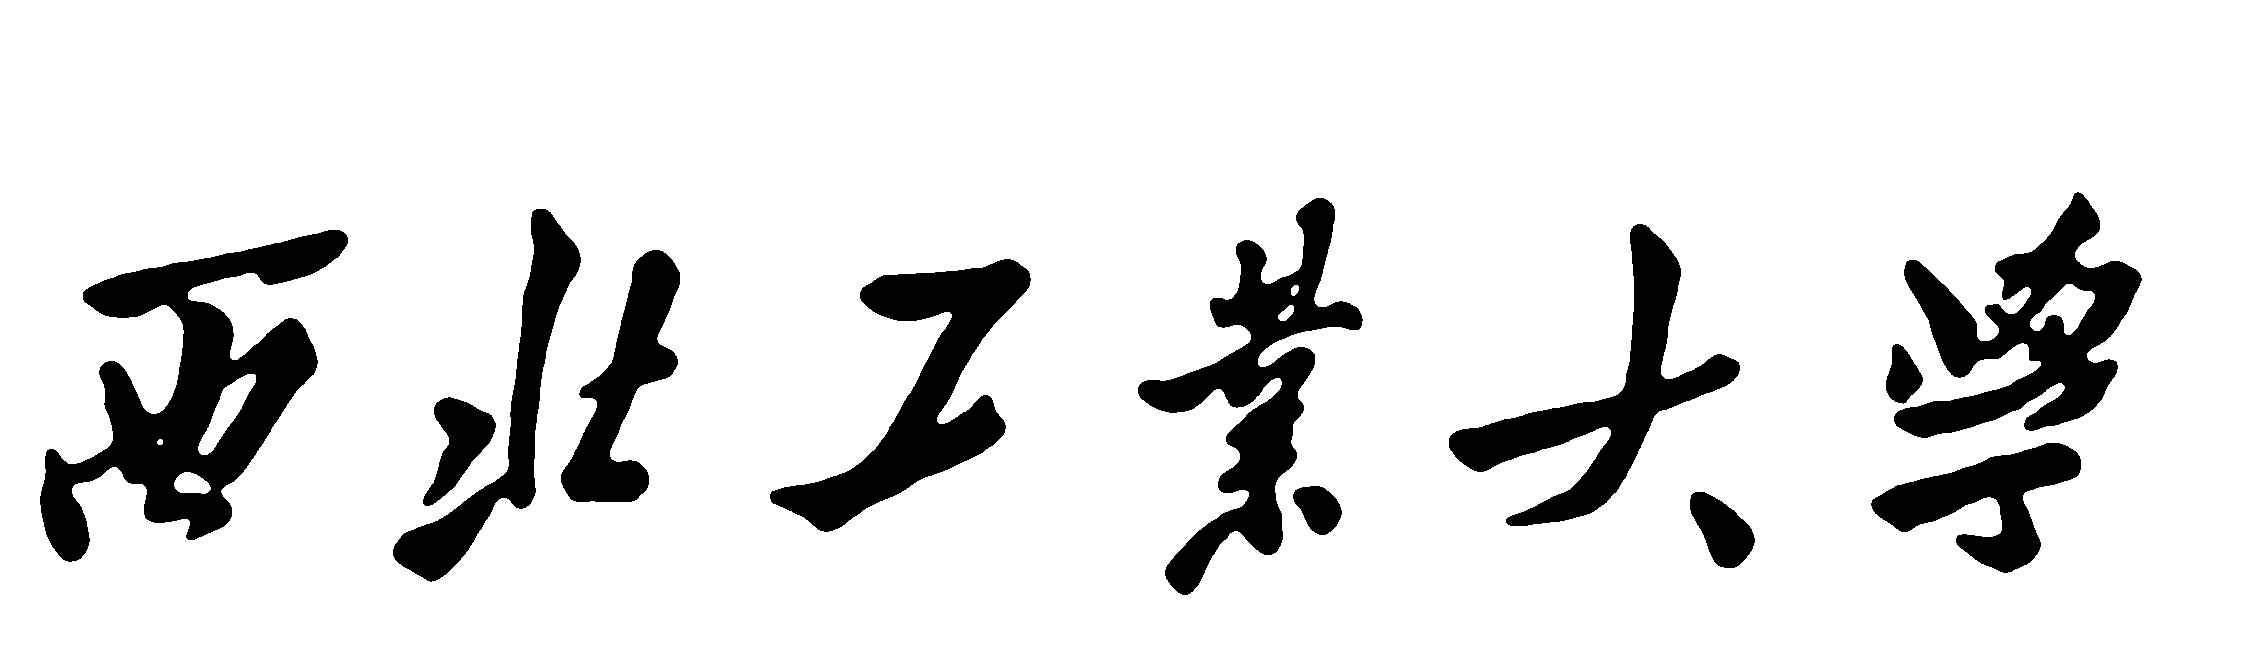
\includegraphics[width=0.5\textwidth]{pic/npu_2.png}\par
        \vspace{1em}
        
\includegraphics[width=0.5\textwidth]{pic/npu_1.png}\par
    \vspace{1em}
        \begin{center}
            \Huge \heiti \textbf{离散数学}

            Discrete Mathematics
        \end{center}
        \vspace{17em}
        \begin{center}
        \songti
        \kaishu 软件学院 \, \heiti\textbf{钱锋} \quad \songti 编
        \vspace{0.5em}

    \today
    \end{center}
\end{titlepage}
\cleardoublepage
\maketitle
\cleardoublepage

\frontmatter
\newpage
\pagestyle{plain}
\makeatother


\chapter{前言}
\thispagestyle{empty}

\subsection*{本书的内容组织}

{
% \captionof{table}{本书的内容结构及其在《离散数学及其应用》中的对应章节} % 表格标题
\begin{longtable}{p{0.35\textwidth}|p{0.6\textwidth}}
    \toprule
    % 表头
    \textbf{章节内容} & \textbf{《离散数学及其应用》中的对应章节} \\
    \midrule
    \endhead
    \bottomrule
    \endfoot

    % 表格内容
    命题与逻辑符号 & 1.1.1、1.1.2、1.1.3、1.1.4、1.1.5、1.3.1、1.3.2 \\
\end{longtable}}



% 离散数学是以研究离散量的结构和相互间的关系为主要目标的数学分支,
% 是综合了分析学、代数学、集合论、数理逻辑、关系论、函数论、图论与组合数学的综合性学科.

\newpage
\thispagestyle{empty}

% 设置目录页的页码格式
\pagenumbering{roman} % 切换回罗马数字页码
\addtocontents{toc}{\protect\thispagestyle{empty}}
\pagestyle{plain}
{\tableofcontents}
\newpage
\thispagestyle{empty}
\cleardoublepage % 确保正文从奇数页开始


% 设置章节标题页的页眉和页脚为空白页样式
\makeatletter
\let\ps@plain\ps@empty
\makeatother

\mainmatter

\chapter{一些通用的数学概念与记号}

在正式开始离散数学的学习之前, 我们首先给出一些通用的数学概念和记号的定义及其用法.
这些概念中的一部分会在后续的课程中得到更进一步的讨论, 在这里提前引入它们唯一的目的
是方便我们的理论推理和表述. 你可以简单粗暴地理解为 —— 我们将在这一章学习一些基本概念的
“高层语义”, 然后在后续的课程中再逐一地讨论这些概念的 “底层原理”\footnote{
    笔者编写的每一本数学讲义中都有本章, 但不同的数学课程在讲授本章时的侧重点和以及讲授范围
    不同.
}.

这样处理的好处是显然的, 因为这可以极大地避免 {\kaishu 强行将相互关联的课题生硬的切分为几个
专题所带来的割裂感和不便}. 此外, 从人脑认知的层面上来说, 我们所掌握的, 或者说会用的东西,
往往都比我们能够清晰地了解的东西要多. V.A. Zorich 在其《数学分析》\cite{zorich1} 中引用的一句俄罗斯古语
就很能说明问题: {\kaishu “当蜈蚣在尝试解释自己为什么有这么多条腿的时候, 连路都不会走了”}.
此外, 这样处理并不会降低表述的严谨程度, 当一个结论需要被严格证明的时候, 我们绝对不会使用
原本没有被证明过的结论来充当论据, 因此对于本书的严谨性而言, 各位读者大可放心.

总而言之, 先学会使用这些概念, 再逐一地针对这些课题展开讨论, 从学习的层面上来说是有益的.

此外, 我们虽然会提及这些概念的定义, 但并不会完全的从头开始, 也就是说, 这一章节的内容
需要中学数学必修课的知识作为先导.

\section{命题与逻辑等价式}

我们平常使用的自然语言是具有二义性的, 而逻辑规则能够给出数学语句的准确含义, 这些语句
可以用来区分数学论证的有效或无效.
逻辑不仅对于理解数学推理十分重要, 而且在计算机科学中有许多应用. 这些逻辑规则用于
计算机电路设计、计算机程序构造、程序正确性验证以及许多其他方面.

本节介绍命题逻辑, 它是由 2300 多年前的古希腊哲学家 Aristotle\footnote{
    亚里士多德(Aristotle)是古希腊最重要、最具影响力的哲学家之一, 他出生于前384年, 在人类思想史上留下了深远的印记.  Aristotle 是柏拉图 (Plato) 的学生, 也是 Plato 学派的成员, 但后来他发展出了自己独特的哲学体系. 他的学术贡献涵盖了众多领域, 包括形而上学、逻辑学、伦理学、政治学、物理学、生物学等等. 

    在形而上学领域,  Aristotle 提出了著名的四因说, 认为一切事物的存在都可以归因于材料因、形式因、动力因和目的因. 他还阐述了“实在”的概念, 主张通过观察和经验来理解世界. 

    在逻辑学方面,  Aristotle 建立了经典的三段论逻辑, 奠定了逻辑学的基础, 并提出了逻辑思维的一系列规则. 

    在伦理学和政治学领域, 他强调了人类的幸福和道德美德的重要性, 并提出了“中庸之道”的理念, 主张在行为中追求适度和平衡. 

    在自然科学方面,  Aristotle 提出了大量的理论和观察, 涉及天文学、生物学、物理学等多个领域. 尽管他的一些理论已经被现代科学所否定, 但他对科学方法和思维的贡献仍然具有重要意义. 

     Aristotle 的思想在西方哲学史上产生了深远的影响, 他的作品被视为西方哲学的经典之一, 其影响持续至今. 
} 系统的创建的.

\subsection{命题的概念}

\subsubsection{命题及其真值}

要把复杂的数学概念和理论阐释清楚, 我们需要使用一些逻辑符号来构造和
描述\textbf{命题} (statement), 所谓命题, 就是一个能够被声明为真或者声明为假的陈述句,
我们把一个命题的真与假称为命题的\textbf{真值} (truth value), 记为 $\mathbf{T}$ 或 
$\mathbf{F}$,
一个命题的真值是且只能是 $\mathbf{T}$ 或 $\mathbf{F}$ 中的一个, 
命题的真值不存在其他的任何情况, 也不存在既真又假的命题.

这就是说, 命题的真值具有唯一性和二值性. 唯一性是指, 命题的真值是唯一确定的, 它要么为真
(对应于 $\mathbf{T}$) 要么假 (对应于 $\mathbf{F}$), 不存在真值不确定的命题, 也不存在
没有真值的命题或者既真又假的命题. 二值性是指, 命题的真值要么是 $\mathbf{T}$ 要么是 $\mathbf{F}$,
关于这一点在前文中已经强调过多次了, 这里不再赘述. 正由于命题真值的二值性,
命题逻辑又称为二值逻辑.

% 关于命题, 我们需要明确的是:
% \begin{enumerate}[label=(\arabic*), itemsep=0pt]
%     \item 命题是一个陈述句, 所以任何疑问句、祈使句等其他句型的句子都不是命题.
%     例如, “今天下雨了” 是一个命题, 但 “明天会下雨吗?” 和 “下雨了请带一把伞”
%     不是命题.
%     \item 命题应该能够被明确地声明真值, 例如, “这句话是一句谎言” 就不是一个命题,
%     事实上, 如果 “这句话是一句谎言” 是真的, 那么这句话的确是一句谎言, 矛盾了; 如果
%     “这句话是一句谎言” 是假的, 那么也就是说这句话是真的, 又矛盾了.
%     这是个非常经典但非常极端的不是命题的例子, 就算你被绕晕了也没有关系,
%     因为在正常的语境当中, 我们能很容易地根据上下文来做出一些相应的判断.
%     \item 命题往往是具有上下文依附性的, 例如, 在 $x=3$ 的语境下, $x+2=5$ 是一个
%     真命题, 但在 $x=5$ 的语境下, $x+2=5$ 就显然是一个假命题了\footnote{
%         请注意, 我们现在并没有严格地定义加法, 但我们在这一章中所做的事情其实
%         只是把我们感性认知的一些概念用用严谨的方式叙述一遍, 过分的钻 “还没有
%         定义加法就不能举这样的例子” 的牛角尖是没有意义的, 请记住, 实践产生认
%         识, 认识再反作用与实践, 我们所接触到的事物往往比我们能够清楚认识的事
%         物要多.}.
% \end{enumerate}
% \begin{example}
%     华盛顿特区是美国的首都.
% \end{example}
% \begin{example}
%     地外文明是存在的.
% \end{example}
% \begin{remark}
%     需要注意的是, 命题是 “可以判断真假的陈述句”, 因此在讨论一个语句是不是命题时, 首先要看
%     该语句是不是陈述句, 其次要看该陈述句是否有确定的真值. 需要注意的是, 我们这里仅仅关注
%     这个语句是否 “具有” 真值, 而对于真值是真是假, 或者是否能够确定, 我们并不关心.
%     因此我们在这里并不关心地外文明的存在性是否有了结论, 也不关心我们是否有能力去得到这个命题的
%     真值. 这种真值暂不明确的命题常称为\textbf{假设}或\textbf{猜想}, 在数学中有许多尚未证明
%     或证伪的命题, 例如著名的 Goldbach 猜想, Riemann 猜想, $3n+1$ 问题....
% \end{remark}
% \begin{remark}
%     在高级程序设计语言中, 命题通常用 \lstinline|boolean| 型变量来定义.
% \end{remark}



% \begin{example}
%     {\kaishu 中国是一个人口众多的国家}. 这是一个陈述句, 并且在特定的语境下能够判断其陈述内容
%     的真假, 例如在上下文中有关于 “人口众多” 的定义和明确的判定标准时, 这个陈述句就是可以
%     明确判定真假的, 因此它是一个命题. 除此之外, 根据常识可知, 中国是目前人口最多的国家,
%     当然称得上是人口众多 (毕竟都已经是最多的那一个了, 再算不上众多的话说明众多的定义需要
%     修正一下了), 所以这是一个真命题.
% \end{example}


% \begin{example}
%     {\kaishu 存在最大的素数}. 这是一个典型的数学命题, 根据素数的有关研究结果我们
%     知道它是一个假命题.
% \end{example}


% \begin{example}
%     {\kaishu 这座楼可真高啊}. 这是一个感叹句, 因此它不是一个命题. 如果改成 “这座楼有
%     超过 50 层” 的话就是一个命题了.
% \end{example}


% \begin{example}
%     {\kaishu 请你跟我走}. 这是一个祈使句, 它不是命题.
% \end{example}


% \begin{example}
%     {\kaishu 火星上也有人}. 这是一个陈述句, 并且是能够判断它的真假的 —— 有人, 或者没有人,
%     必居其一且只居其一, 所以这是一个命题. 虽然目前我们的科学研究并不能严格的说明火星上
%     是否有人存在, 但是按照目前的主流观点来看, 火星上是没有人的, 所以我们说这个命题
%     在这意义下是一个假命题.
% \end{example}

\subsubsection{逻辑常量与逻辑变量 \quad 真值表}

我们把 $\mathbf{T}$ 和 $\mathbf{F}$ 称为\textbf{逻辑常量} (logical constant),
把命题称为\textbf{逻辑变量} (logical variable) 或者命题变量、语句变量. 习惯上我们用字母
$p,q,r, \cdots$ 来表示命题变量. 命题变量 $p$ 的真值为 $\mathbf{T}$, 记作
\[ p = \mathbf{T}, \]
有时我们也用 $p$ 的符号本身来代表 $p$ 是一个真命题. 例如说, 令 $x=3$, $p$ 表示 $x>2$, 
那么 $x>2$ 显然是成立的, 这时不必再麻烦地写出 $(x>2) = \mathbf{T}$, 直接写 $x>2$ 即可.

不能再分解为更简单的陈述句的命题成为\textbf{原子命题} (atom proposition),
由原子命题 $x_1, x_2, \cdots, x_n$ 通过逻辑连接词连接得到的命题
$p(x_1, x_2, \cdots, x_n)$ 称为\textbf{复合命题}. 

\begin{definition}[复合命题]
    复合命题 $p(x_1, x_2, \cdots, x_n)$ 可以递归地定义如下:
    \begin{enumerate}[label={$\left.\arabic*\right)$}, itemsep=0pt]
        \item $x_1, x_2, \cdots, x_n$ 是命题;
        \item 如果 $a, b$ 是命题, $\circ$ 是一个逻辑连接词, 那么 $a \circ b$
        也是命题.
    \end{enumerate}
\end{definition}



复合命题的真值是由其所对应的原子命题 $x_1, x_2, \cdots, x_n$ 的一个取值组合确定的, 这样的一个取值组合形如
$(\mathbf{T}, \mathbf{F}, \cdots, \mathbf{T})$, 我们将其称为一个\textbf{指派}.
如果我们用符号 $1$ 来表示逻辑常量 $\mathbf{T}$, 用符号 $0$ 来表示逻辑常量 $\mathbf{F}$ 的话,
一个指派实际上可以用一个形如 $10\cdots1$ 的比特串来表示. 我们通常用一张称为\textbf{真值表}
(truth table) 的表格来表示复合命题和与其对应的原子命题的一个指派之间的关系.

\begin{example}
    \label{与非运算}
    我们可以利用真值表定义复合命题 $y = p(x_1, x_2)$ 为如表 \ref{example: truth-table} 所示形式:
    {
    \captionof{table}{复合命题 $y = p(x_1, x_2)$ 的真值表} % 表格标题
    \label{example: truth-table} % 交叉引用标签
    \begin{longtable}{cc|c}
        \toprule
        % 表头
        $x_1$ & $x_2$ & $y$ \\
        \midrule
        \endhead
        \bottomrule
        \endfoot
    
        % 表格内容
        0 & 0 & 1 \\
        0 & 1 & 1 \\
        1 & 0 & 1 \\
        1 & 1 & 0 \\
    \end{longtable}}
    从本例容易看出, 在复合命题的真值表中, 一个原子命题对应于一列, 而一个指派则对应于一行.
    在处理一些由命题连接词连接成的复合命题时, 我们还可以在真值表中插入若干的列,
    这些列上的命题是我们在利用连接词复合命题的过程中产生的中间逻辑变量.

    有时为了节约纸张空间, 我们也会把真值表写成一种更 “扁平” 的形式, 在这里我们需要使用
    函数的映射关系符号 (用 $\mapsto$ 表示), 所以 $y$ 实际上也可以写成
    \[ y: \left\{
        00 \mapsto 1,
        01 \mapsto 1,
        10 \mapsto 1,
        11 \mapsto 0
    \right\}. \]
    不难看出这个写法实际上定义了一组对应关系, 把一个比特串对应到了一个逻辑常量,
    它与我们在程序设计语言中的 \lstinline|switch-case| 语句\footnote{
        如果读者想要了解有关程序设计语言中的 \lstinline|switch-case| 语句的更多内容,
        可以参阅笔者编写的《程序设计基础 (C)》.
    }实际上是一致的.
\end{example}

\subsection{逻辑连接词 \quad 逻辑运算符}

\subsubsection{逻辑连接词}

使用逻辑连接词可以用若干原子命题构造出各种各样复杂的命题, 事实上, 在我们的自然语言中
也有这样的逻辑连接词, 它们通常用来表示语句中元素的并列关系、转折关系, 等等. 接下来要介绍的
逻辑连接词, 正是这些自然语言词语的更精确的表达.

\begin{definition}[命题连接词]
    常用的五个逻辑联结词是 “与”、“或”、“非”、“蕴含” 和 “具有相同的真值”.
    \begin{enumerate}[label={$\left.\arabic*\right)$}, itemsep=0pt]
        \item $\lnot p$ 或者 $\bar p$ 称为 $p$ 的\textbf{逻辑否定} (logical negation, logical NOT) 或者逻辑非.
        \item $p \wedge q$ 称为 $p,q$ 的\textbf{合取命题} (conjunction, logical AND),
        有时也称命题的合取为命题的乘法, 合取命题为命题的\textbf{逻辑积} (logical product), 
        并且把 $p \wedge q$ 像代数积一样写作 $pq$.
        \item $p \vee q$ 称为 $p,q$ 的\textbf{析取命题} (disjunction, logical OR),
        有时也称命题的吸取为命题的加法, 析取命题称为命题的\textbf{逻辑和} (logical summation),
        并且把 $p \vee q$ 像代数和一样写作 $p+q$. 
        \item $p \rightarrow q$ 称为 $p$ \textbf{蕴含} (imples) $q$,
            $p \to q$ 也称为 $p$ 到 $q$ 的\textbf{蕴含式} (implication) 或条件语句.
        \item $p \leftrightarrow q$ 表示 {\kaishu $p$ 与 $q$ 具有相同的真值}, 也称为 $p$ 与 $q$ 的\textbf{双条件语句} (logical biconditional).
    \end{enumerate}
    其中, 除逻辑非是一元逻辑连接词外, 其余的四个连接词都是二元连接词. 这些命题可以通过逻辑
    连接词复合成新的命题, 这些连接成的命题的真值表如表 \ref{常用逻辑连接词的真值表} 所示:
    \begin{table}[H]
        \centering
        \caption{常用逻辑连接词的真值表}
        \label{常用逻辑连接词的真值表}
        \begin{tabular}{cc|ccccc}
            \toprule
            $p$ & $q$ & $\lnot p$ & $p \wedge q$ 
            & $p \vee q$ & $p \to q$ & $p \leftrightarrow q$ \\
            \midrule
            0 & 0 & 1 & 0 & 0 & 1 & 1\\ 
            0 & 1 & 1 & 0 & 1 & 1 & 0\\ 
            1 & 0 & 0 & 0 & 1 & 0 & 0\\ 
            1 & 1 & 0 & 1 & 1 & 1 & 1\\ 
            \bottomrule
        \end{tabular}
    \end{table}
\end{definition}


根据上表可知, $p \wedge q$ 为真当且仅当 $p,q$ 同时为真, 而 $p \vee q$ 为假当且仅当
$p,q$ 同时为假. $\lnot p$ 与 $p$ 的真值总是相反的, 所以 “非” 也称为 “取反”, 
而 $p \leftrightarrow q$ 为真当且仅当 $p,q$ 具有相同的真值.

关于 $p \rightarrow q$, 我们有一个 “善意的推定”, 那就是当蕴含式的前件是假命题
的时候, 后件无论是真是假, 整个蕴含式都是真的. 比如说, “如果你考了第一名, 我就带你去吃大餐”,
“如果我是国家主席, 我就把科研人员的收入标准提高到第一梯队上”, 当前件为假命题的时候, 就算后面
是在胡说八道, 这也是一个真命题. 所以那些虚伪的政客会做出各种各样的承诺来诱惑你, 你可能会怀疑
这个政客上台后是否真的会兑现这个诺言, 但你不可否认的是, 它是一个有效的承诺.

在有些参考书中, 双条件语句 $p \leftrightarrow q$ 又称为 “$p$ 与 $q$ 的等价式”,
但注意到这一节的标题了吗? 对于初学者而言, 这个称呼可能会与 “逻辑等价式” 的概念产生混淆,
因此在本书中我们统一采用 {\kaishu $p$ 与 $q$ 具有相同的真值}来解释 $p \leftrightarrow q$.
而将 $p \leftrightarrow q$ 称为 “双条件语句” 其实是合理的, 这是因为 $p \leftrightarrow q$
实际上就是 $(p \to q) \wedge (q \to p)$, 事实上, 无论 $p,q$ 给出怎样的指派,
$p \leftrightarrow q$ 与 $(p \to q) \wedge (q \to p)$ 总具有相同的真值,
这其实就是我们很快就要学到的 “逻辑等价”.

\subsubsection{逻辑函数}

利用这五种逻辑联结词的组合, 我们可以建立各种各样的复合逻辑命题. 当一个二元复合逻辑命题
的真值可以与 $00$, $01$, $10$, $11$ 四种指派建立对应关系时, 我们称这个二元复合逻辑命题
为一个二元\textbf{逻辑运算符} (logical operation).
容易看出, 逻辑连接词中的 $\vee, \wedge, \to, \leftrightarrow$ 都是二元逻辑运算符.
而逻辑否定的真值则可以与 $0$, $1$ 建立对应关系, 它是一元逻辑运算符.

\begin{example}
    在例 \ref{与非运算} 中展示的复合命题所对应的逻辑表达式应该为 $\lnot(x_1 \wedge x_2)$
    或 $\overline{x_1x_2}$. 它是两个逻辑命题首先相与, 再取否定的结果, 因此这一运算
    也称为\textbf{与非} (AND-NOT) 运算.
\end{example}
\begin{example}
    两个命题 $x_1, x_2$ 首先相或, 然后取否定得到的结果 $\lnot(x_1 \vee x_2)$ 或
    $\overline{x_1 + x_2}$ 实际上也定义了一个逻辑运算符, 
    我们称其为\textbf{或非} (OR-NOT) 运算. 或非运算的真值为
    \[ \left\{ 00 \mapsto 1, 01 \mapsto 0, 10 \mapsto 0, 11 \mapsto 0 \right\}. \]
\end{example}
\begin{example}
    逻辑或实际上包含了两种情况, 其一是 $p$ 与 $q$ 中有且仅有一个 $1$, 其二是 $p$ 与
    $q$ 同时为一. 这种 “或” 实际上是\textbf{兼或} (inclusive or), 它表示二者同时为真
    时我们也认为析取命题为真. 与兼或相对应的是\textbf{异或} (exclusive or), 它表示
    $p$ 与 $q$ 中有且仅有一个 $1$, 即 $p \bar q + q \bar p$. 异或运算记作 $p \oplus q$. 它的真值为
    \[ \left\{ 00 \mapsto 0, 01 \mapsto 1, 10 \mapsto 1, 11 \mapsto 0 \right\}, \] 
    可以看出, $p$ 异或 $q$ 为真当且仅当 $p$ 与 $q$ 具有相反的真值.
    双条件语句 $p \leftrightarrow q$ 为真当且仅当 $p$ 与 $q$ 具有相同的真值,
    注意到这恰好与异或运算的要求相反,
    因此我们也称双条件运算符为\textbf{同或}运算.
\end{example}

更一般地, 假设 $x_1, x_2, \cdots, x_n$ 是 $n$ 个逻辑变元,
$p$ 是一个逻辑变量. 如果对于这些命题变元的每一个指派, $p$ 都有唯一确定的真值与之对应,
则称 $p(x_1, x_2, \cdots, x_n)$ 是一个\textbf{逻辑函数} (logical function) 
或 $n$ 元逻辑谓词, 它的真值是由逻辑变元 $x_1, x_2, \cdots, x_n$ 的一个组合所唯一确定的.
二元逻辑函数也常称为二元逻辑运算符, 这是因为我们恰好可以把一个符号 $\circ$ 写到参与运算的
两个逻辑变元中间.

% \begin{example}
%     设 $p$ 为 $2$ 是素数, $q$ 为 $3$ 是素数, $r$ 为 $\sqrt{2}$ 为有理数.
%     下列符合命题中哪一个是假命题?
%     \begin{itemize}[itemsep=0pt]
%         \item $(p \vee q) \rightarrow r$. 我们先判断一下 $p,q,r$ 的真值,
%         显然 $p=1,q=1,r=0$, 于是 $(p \vee q) = 1$, 根据蕴含式的真值规则,
%         前件为真, 后件为假, 该命题为假命题.
%         \item $r \rightarrow (p \vee q)$. 根据蕴含式的真值规则, 当前件为假时
%         无论后件为真命题还是假命题, 蕴含式为真, 所以由 $r=0$ 知这是一个真命题.
%         \item $(p \wedge q) \rightarrow p$. 根据合取式的真值表, $(p \wedge q)=1$,
%         前件为真, 后件为真, 这是一个真命题.
%         \item $(r \vee p) \leftrightarrow q$. 根据 $p,q,r$ 的真值可知,
%         $(r \vee p)=1, q=1$, 于是根据等价式的真值规则, 这是一个真命题.
%     \end{itemize} 
% \end{example}

% \begin{example}
%     设命题 $p,q$ 的真值为 F, 命题 $r,s$ 的真值为 T, 求公式 $(p \leftrightarrow r)
%     \wedge ((\lnot q) \vee s)$ 的真值.
%     \begin{sol}
%         直接代入 $p,q,r,s$ 的真值, 得到
%         \[ (0 \rightarrow 1)\wedge((\lnot 0) \vee 1), \]
%         根据等价式和逻辑或的真值规则, 它实际上就是
%         \[ 0 \wedge 1, \]
%         根据逻辑与的运算规则, 原命题的真值应该为 F.
%     \end{sol}
% \end{example}

% \begin{example}
%     设命题 $p$ 为 “天气冷”, 命题 $q$ 为 “小王穿羽绒服”. 那么, “只要天冷, 小王就穿
%     羽绒服” 记作 $p \rightarrow q$, 而 “只有天冷, 小王才穿羽绒服”, 这句话的意思是
%     如果不是冷天的话, 小王就不穿羽绒服了, 这与 $p \rightarrow q$ 是不一样的,
%     $p \rightarrow q$ 的意思是就算不是冷天, 小王也有可能也穿了羽绒服, 因此这句话
%     应该写作 $q \rightarrow p$. 
% \end{example}

\subsubsection{逻辑函数的数量}

根据逻辑运算符的概念, 我们能够看出逻辑运算符的数量实际上参与运算的逻辑变量的数量是相互对应的.
根据组合数学的知识可以知道, 一个逻辑变元对应 $2$ 种指派, 逻辑变元的取值又有 $2$ 种可能,
所以一元逻辑函数一共有 $2^2 = 2^{2^1}= 4$ 个, 我们分别用 $L_1, L_2, L_3, L_4$ 来表示:
{\captionof{table}{一元逻辑函数} % 表格标题
\label{一元逻辑函数} % 交叉引用标签
\begin{longtable}{c|cccc}
    \toprule
    % 表头
    $x$ & $L_1$ & $L_2$ & $L_3$ & $L_4$ \\
    \midrule
    \endhead
    \bottomrule
    \endfoot

    % 表格内容
    0 & 0 & 0 & 1 & 1 \\
    1 & 0 & 1 & 0 & 1 \\
\end{longtable}}
其中, $L_1$ 和 $L_4$ 分别是逻辑常量 $\mathbf{F}$ 和 $\mathbf{T}$.
$L_2$ 则是 $x$ 本身, $L_3$ 实际上是 $\bar x$. 因此, 任意的一个一元逻辑函数实际上都可以
由逻辑常量 $\mathbf{T}, \mathbf{F}$ 和逻辑否定运算符 $\lnot$ 表示出来.

二元逻辑函数的情况略微复杂一些. 二元逻辑函数有 $2^4 = 4$ 种指派, 而每个逻辑变元的取值又有
$2$ 种可能, 因此二元逻辑函数实际上有 $2^4 = 2^{2^2} = 16$ 中, 我们分别用
$L_1, L_2, \cdots, L_{16}$ 来表示:
\begin{table}[H]
    \centering
    \caption{二元逻辑函数}
    \begin{tabular}{cc|cccccccccccccccc}
        \toprule
        $x$ & $y$ & $L_1$ & $L_2$ & $L_3$ & $L_4$ & $L_5$ & $L_6$ & $L_7$ & $L_8$ & $L_9$ & $L_{10}$ & $L_{11}$ & $L_{12}$ & $L_{13}$ & $L_{14}$ & $L_{15}$ & $L_{16}$ \\
        \midrule
        0 & 0 & 0 & 0 & 0 & 0 & 0 & 0 & 0 & 0 & 1 & 1 & 1 & 1 & 1 & 1 & 1 & 1 \\
        0 & 1 & 0 & 0 & 0 & 0 & 1 & 1 & 1 & 1 & 0 & 0 & 0 & 0 & 1 & 1 & 1 & 1 \\
        1 & 0 & 0 & 0 & 1 & 1 & 0 & 0 & 1 & 1 & 0 & 0 & 1 & 1 & 0 & 0 & 1 & 1 \\
        1 & 1 & 0 & 1 & 0 & 1 & 0 & 1 & 0 & 1 & 0 & 1 & 0 & 1 & 0 & 1 & 0 & 1 \\
        \bottomrule
    \end{tabular}
\end{table}

其中, $L_1$ 和 $L_{16}$ 分别是逻辑常量 $\mathbf{F}$ 和 $\mathbf{T}$.
$L_4$ 实际上是逻辑变量 $x$, $L_6$ 实际上是 $y$, $L_{13}$ 是 $\bar x$, $L_{11}$ 是
$\bar y$. $L_2$ 是 $xy$, 即 $x$ 与 $y$ 的合取命题, $L_8$ 是 $x+y$, 即 $x$ 与 $y$
的析取命题. $L_{14}$ 是 $x \to y$, 而 $L_3$ 则是 $\overline{x \to y}$.
$L_{12}$ 是 $y \to x$, 而 $L_5$ 则是它的否定, 即 $\overline{y \to x}$.
$L_{10}$ 实际上是 $x \leftrightarrow y$, 而 $L_{7}$ 则是它的否定, 即 $x$ 与 $y$
的异或 $x \oplus y$. $L_{15}$ 是 $x$ 和 $y$ 的与非 $\overline{xy}$,
而 $L_9$ 则是 $x$ 和 $y$ 的或非 $\overline{x+y}$.

不难发现, 任意一个二元逻辑函数都可以用 $\mathbf{T}$, $\mathbf{F}$ 和 $\lnot,
\wedge, \vee, \to, \rightarrow$ 表示. 我们称它们对于二元逻辑函数来说是 “完备的”.
事实上, 可以把这个完备的运算符集合进一步缩小, 但讨论它的应用价值不高, 这里就先不再过多的深入讨论了.

一般地, $n$ 元逻辑函数有 $2^{2^n}$ 个. 这里要注意指数的结合是从右向左的, 也就是说 $n$ 先
作为 $2$ 的指数, 然后 $2^n$ 再作为 $2$ 的指数. 如果你觉得这种写法有些难以辨认的话,
可以写作 $\exp_2(2^n)$, 这种写法清晰的分离了指数部分和底数部分, 具有更强的可读性\footnote{
    一般地, 以 $a$ 为底, $x$ 为指数的指数幂可以写作 $\exp_a(x)$ 的形式, 以 $\mathrm{e}$
    为底的自然指数则可以直接写作 $\exp(x)$.
}.

\subsection{逻辑运算符的优先级}

五个逻辑运算符的优先级从高到低排序如下所示:
\[ \lnot, \quad \wedge, \quad \vee, \quad \to, \quad \leftrightarrow, \]
总的来说, 首先, {\kaishu 否定运算符优先于所有的其他逻辑运算符}, 我们亲切地称
否定运算符处于逻辑运算符优先级的 “第一梯队”. 其次, {\kaishu 合取运算符则优先于析取运算符},
这从我们把合取命题写作 $pq$ 而把析取命题写作 $p+q$ 也能看出来, 它们处于 “第二梯队”.
第三, 条件运算符和双条件运算符低于否定、合取和析取, 它们处于 “第三梯队”,
其中, {\kaishu 条件运算符优先于双条件运算符}.

简单的来说, 你可以把这些规则记作 “非与或蕴双”.

\subsection{自然语言与逻辑命题之间的相互翻译}

% \begin{example}
%     在 $\mathbb{R}^n$ 中, 向量组 $\boldsymbol{a}_1,\boldsymbol{a}_2,\cdots,
%     \boldsymbol{a}_s$ 线性无关的定义是, 只有组合系数全为 $0$ 时它们的线性组合才为
%     零向量 $\boldsymbol{0}$. 这就是说, 从 $k_1\boldsymbol{a}_1 +
%     k_2\boldsymbol{a}_2 + \cdots + k_s\boldsymbol{a}_s = \boldsymbol{0}$
%     能推出 $k_1 = k_2 = \cdots = k_s = 0$.
%     你看, “只有” 后面跟着的, 是被推出来的那个, 所以千万不要记混了.
% \end{example}

\begin{example}
    {\kaishu 虽然交通堵塞, 但是老王还是准时到达火车站}. 设 $p$ 为交通拥堵,
        设 $q$ 为老王准时到达火车站. 显然这里的转折关系是表示这两件事情同时发生的,
        因此应该取它们二者的合取命题, 即 $p \wedge q$.
\end{example}

\begin{example}
    {\kaishu 张小宝是三好生, 它是北京人或河北人}. 设 $p$ 为张小宝是三好生,
        $q$ 表示张小宝是北京人, $r$ 表示他来自河北. 这里的逗号显然表示了并列关系,
        因此应该取 $p \wedge (q \vee r)$.
\end{example}

\begin{example}
    {\kaishu 除非天下雨, 否则我骑车上班}. 这句话的意思就是说, 如果天不下雨那么我就要
        骑车去上班, 设 $p$ 表示雨天, $q$ 表示我骑车去上班, 那么表示为
        $(\lnot p) \rightarrow q$.
\end{example}

\subsection{永真式 \quad 逻辑等价式}

\begin{definition}
    一个真值永远是真的复合命题 (无论其中出现的命题变量的真值是什么)
    称为\textbf{永真式} (tautology)\footnote{
        永真式的英文是 tautology, 谐音是 “套套逻辑”, 请你不要想歪……
        然而, 在有些逻辑学参考书中, 将套套逻辑解释为类似 “用结论证明结论”
        的循环论证, 这个解释也是合理的, 因为循环论证就像一个圆环一样 “套” 起来了.
    }. 真值永远为假的复合命题称为\textbf{矛盾式} (contradiction).
    既不是永真式, 又不是矛盾式的复合命题称为\textbf{可能式} (contingency).
\end{definition}

\begin{definition}
    设 $p$ 和 $q$ 是两个逻辑命题, 如果 $p \leftrightarrow q$ 是永真式,
    即 $p$ 与 $q$ 总是具有相同的真值, 则称 $p$ 与 $q$ 是\textbf{逻辑等价}
    (logical equivalent) 的, 记作
    $p \equiv q$.
\end{definition}

\begin{remark}
    符号 $\equiv$ 并不是一个逻辑联结词, 所以 $p \equiv q$ 不是一个复合命题,
    你可以认为, $\equiv$ 是两个逻辑命题 $p,q$ 之间的一种 “关系”. 有时候我们也把
    $p \equiv q$ 记作 $p \Leftrightarrow q$.
\end{remark}

复合命题 $p,q$ 逻辑等价当且仅当它们在真值表上所对应的两列完全相同.

\begin{example}[De Morgan]
    $\lnot (p \wedge q) \equiv (\lnot p) \vee (\lnot q)$,
    \quad 
    $\lnot (p \vee q) \equiv (\lnot p) \wedge (\lnot q)$.
    \begin{proof}
        我们把这两个命题的及其对应的原子命题的真值表列出来,
        \begin{center}
            \begin{tabular}{cc|cccccccc}
                \hline
                $p$ & $q$ & $\lnot p$ & $\lnot q$ & $p \wedge q$ & $p \vee q$ &
                $\lnot(p \wedge q)$ & $\lnot(p \vee q)$ 
                & $(\lnot p) \vee (\lnot q)$
                & $(\lnot p) \wedge (\lnot q)$ \\
                \hline 
                0 & 0 & 1 & 1 &  & 0 & 1 & & 1 &\\ 
                0 & 1 & 1 & 0 &  & 1 & 1 & & 1 &\\ 
                1 & 0 & 0 & 1 &  & 1 & 1 & & 1 &\\ 
                1 & 1 & 0 & 0 &  & 1 & 0 & & 0 &\\
                \hline
            \end{tabular}
        \end{center}
    我们注意到 $\lnot(p \wedge q)$ 与 $(\lnot p)\vee(\lnot q)$ 所在的列
    完全相同, 这说明 
    $\lnot (p \wedge q) \leftrightarrow (\lnot p)\vee(\lnot q)$
    是永真式, 它们是逻辑等价的, 即 
    $\lnot (p \wedge q) \equiv (\lnot p) \vee (\lnot q)$. 
    现在请你补充真值表上补充剩下的三列,
    证明 $\lnot (p \vee q) \equiv (\lnot p) \wedge (\lnot q)$.
    \end{proof}
\end{example}

\begin{example}
    $p \rightarrow q \equiv (\lnot p) \vee q$.
    \begin{proof}
        我们采用真值表证明,
        \begin{center}
        \begin{tabular}{cc|ccc}
            \hline 
            $p$ & $q$ & $\lnot p$ & $(\lnot p) \vee q$ & $p \rightarrow q$ \\ 
            \hline 
            0 & 0 & 1 & 1 & 1\\ 
            0 & 1 & 1 & 1 & 1\\ 
            1 & 0 & 0 & 0  & 0\\
            1 & 1 & 0 & 1 & 1 \\ 
            \hline
        \end{tabular}
        \end{center}
        真值表中它们所在的两列是完全相同的, 于是我们便证明了 
        $p \rightarrow q \equiv (\lnot p) \vee q$.
        这个逻辑等价式非常重要, 在我们化简逻辑表达式的时候, 常常用它来 “去箭头”.
    \end{proof}
\end{example}

接下来我们列出一些常用的逻辑等价式, 如表 \ref{常用的逻辑等价式} 所示, 请注意, 我们在这里将命题的合取写作了
代数积的形式, 命题的析取写作了代数和的形式, 而把命题 $x$ 的否定写作了 $\bar x$.
这些逻辑等价式都可以通过真值表来得到证明, 我们不再赘述, 各位读者可以自己尝试证明它们,
但是想一想, 你为什么不去做点更有意思的事情呢? 好了, 不扯了, 后面我们会用更优雅的方式
来证明这些等价式的, 因此我们在这里不要求各位独立给出证明, 也不要求各位读者记忆这些逻辑等价式,
各位读者在这里只需要对这些式子做一个大概的了解就好, 在需要的时候再翻回到这里查阅. 
强烈推荐各位读者把这些逻辑等价式和后面即将学到的集合恒等式与布尔代数恒等式对比起来学习.

{\captionof{table}{常用的逻辑等价式} % 表格标题
\label{常用的逻辑等价式} % 交叉引用标签
\begin{longtable}{p{0.33\textwidth}|c||p{0.33\textwidth}|c}
    \toprule
    % 表头
    \textbf{恒等式} & \textbf{名称} & \textbf{恒等式} & \textbf{名称} \\

    \midrule
    \endhead
    \bottomrule
    \endfoot

    % 表格内容
        $\overline{\left(\bar x\right)}  \equiv  x$ & 双重补律 & $x + yz  \equiv  (x+y)(x+z)$
        
        $x(y+z)  \equiv  xy+xz$& 分配律\\
        \hline
        $x+x  \equiv  x$ 

        $x \cdot x  \equiv  x$ & 幂等律 & $\overline{xy}  \equiv  \bar x + \bar y$

        $\overline{x+y} \equiv \bar x \bar y$ & De Morgan 律 \\ 
        \hline
        $x+\mathbf{F}  \equiv  x$

        $x \cdot \mathbf{T}  \equiv  x$ & 同一律 & $x + xy \equiv x$

        $x(x+y) \equiv x$ & 吸收律 \\
        \hline 
        $x + \mathbf{T} \equiv \mathbf{T}$ 

        $x \cdot \mathbf{F} \equiv \mathbf{F}$ & 支配律 & $x + \bar x \equiv \mathbf{T}$ & $\mathbf{T}$ 的性质 \\ 
        \hline 
        $x+y \equiv y+x$

        $xy \equiv yx$ & 交换律 & $x\bar x \equiv \mathbf{F}$ 
        
        $\mathbf{T}$ 与 $\mathbf{F}$ 的性质统称为 “补律” & $\mathbf{F}$ 的性质 \\ 
        \hline 
        $x+(y+z) \equiv (x+y)+z$ 

        $x(yz) \equiv (xy)z$ & 结合律 & & \\ 
\end{longtable}}

\section{集合与集合恒等式}

\subsection{集合与集合中的元素}

\subsubsection{集合中元素的特性}

我们在讨论问题时, 一定范围内所涉及的对象, 例如数、向量、多项式、矩阵、点、直线,
或者桌子上的笔、纸张和水杯, 等等事物, 都可以笼统地称为\textbf{元素} (element),
若干个 (有限个或无限个) 元素所组成的全体, 可以被笼统地称为一个\textbf{集合} (set),
两个集合相等当且仅当它们含有完全相同的元素.
集合中的元素通常用小写拉丁字母表示, 集合通常用大写拉丁字母表述, 我们约定,
如果一个对象 $a$ 是集合 $A$ 的元素, 那么我们称\textbf{$a$ 属于 $A$}, 读作 $a$ belongs to
$A$\footnote{
    大写字母 $A$ 通常读作 capital of $A$, 因此 $a \in A$ 也常读作 $a$ belongs to 
    capital of $A$.
}, 记作 $a \in A$, 否则称 \textbf{$a$ 不属于 $A$}, 记作 $a \notin A$.

集合中的元素具有确定性、互异性和无序性. 确定性要求一个对象是否是某个集合的元素这件事情是确定的,
也就是说, 一个元素 $a$ 要么属于集合 $A$, 要么不属于集合 $A$, 二者必居其一且只居其一.
互异性要求集合中的两个元素是彼此不同的, 即相等的对象 $a$ 和 $b$ 在集合中被视为同一个元素.
无序性指的是, 在一个集合中没有元素之间的次序, 不过你可以人为的在集合上定义一个次序,
定义了序关系的集合称为有序集, 我们常见的数集就是有序集.

需要强调的是, 集合也可以作为其他集合的元素.

\subsubsection{空集与论域}

不包含任何元素的集合称为\textbf{空集} (empty set), 记作 $\varnothing$.
今后在谈到集合的时候, 如果不加以特别说明, 一般指的是非空集合.

我们需要指出的是, “一切事物的集合” 这个集合是不存在的. 这是因为, 如果有一个集合 $A$ 它包含了
一切的事物, 那么当我们把 $A$ 集合当做一个事物去看待 (一个集合也是一个事物, 因此它当然可以被
视为集合的元素) 的时候, 它应该也属于这个 “一切事物的集合”.
这就会涉及到集合包含自身所引起的集合的无穷递归问题, 因此我们不能说有一个包含了一切事物的 “全集”.
但是我们可以定义一个集合来划定一个明确的讨论范围, 例如说 “所有地球人组成的集合”, “所有的实数
组成的集合”, “集合 $\left\{ 0, 1 \right\}$ 的所有子集组成的集合”, 等等. 一般的, 在上下文
能够确定一个明确的讨论范围 (也就是一个集合\footnote{
    稍微了解过公理化集合论的读者应该了解过这样的一句话: 这个世界上除了集合, 什么都没有.
}) 的时候, 由于这个上下文中所有的讨论都是在这个集合及其子集内展开的,
我们把这个讨论的范围称为\textbf{论域} (domain of discourse), 记作 $\varOmega$, 
在概率论中也将其称为\textbf{样本空间}\footnote{
    要注意样本空间也是基于一定的研究客观现象的需要而确定的, 它不是一个 “包含了一切样本点的集合”,
    而只是在特定的研究的问题中可能出现的所有样本点的集合.
} (sample space), 在部分参考资料中也称它为全集 (尽管我并不喜欢这个可能会引起误会的称呼), 
无论如何, 它们指代的都是同一个概念. 总而言之请你记住, 论述域一定是一个确定的集合, 它是根据
我们具体的研究需要而划定的, 不能将其简单粗暴地理解为 “宇宙中所有事物组成的全体”.

\subsection{常见的数集}

我们常用 $\mathbb{N}$ 来表示自然数集 (在本书中它是从 $0$ 开始的), $\mathbb{Z}$ 表示整数集,
$\mathbb{Q}$ 表示有理数集, $\mathbb{R}$ 表示实数集, $\mathbb{C}$ 表示复数集.

在数集符号的右上角标注一个 $+$ 表示这个数集的正子集, 例如 $\mathbb{Z}^+$ 表示正整数集,
它实际上也等于 $\mathbb{N}^+$, 而 $\mathbb{Q}^+, \mathbb{R}^+$ 则分别表示正有理数集
和正实数集. 在数集的右上角标注一个 $*$ 则表示从这个数集中取出元素 $0$ 剩下的部分, 例如
$\mathbb{Z}^*$ 是所有非零整数组成的集合, $\mathbb{R}^*$ 是所有非零实数组成的集合.
这里要注意的是, 由于自然数集 $\mathbb{N}$ 是从 $0$ 开始的, 所以 $\mathbb{N}^*$
实际上与 $\mathbb{N}^+$ 和 $\mathbb{Z}^+$ 是同一个集合.
现在你应该知道为什么中学教材上常常混用 $\mathbb{N}^+$、$\mathbb{N}^*$ 和 $\mathbb{Z}^+$
了, 不过按照笔者个人的习惯, 我更倾向于使用 $\mathbb{N}^+$ 来表示所有的正整数.

\subsection{枚举法和描述法}

我们有两种方法来表示一个集合, 一种是\textbf{枚举法} (roster method), 它的英文的直译
是 “花名册方法”, 顾名思义, 既然是花名册, 那么枚举法的核心自然就是罗列出集合中的元素, 如果是元素数量
很多的集合, 或者是无穷集合,
那么可以使用省略号来避免逐一地列举这些元素, 但如果要这么做的话, 至少要罗列到能够看出其中的规律为止, 例如,
\[\mathbb{N} = \left\{0, 1, 2, \cdots \right\},\]
你应该能很容易看出下面的元素应该是 $3,4,5, \cdots$. 另一种是\textbf{描述法} (set builder),
术语 “builder” 来源于程序设计当中的 “构造器” 或者 “构造函数”, 描述法的核心是写出这一集合的元素
所满足的共同的特征, 例如, 所有小于 $10$ 的奇数的集合 $O$ 可以表示为
\[ O = \left\{ x \in \mathbb{Z} | (x < 10) \wedge (x \equiv 1 \pmod{2}) \right\}, \] 
其中符号 $\wedge$ 表示两个命题的合取, 它表示 $x<10$ 与 $x \equiv 1 \pmod{2}$ 同时成立
(很快我们就会再见到它),
$x \equiv 1 \pmod{2}$ 则表示 $x$ 是一个奇数 (你很快就会知道其中的原因了).

我们要指出的是, 并不是所有的集合都可以用枚举法和描述法来简单地描述的, 不然的话, 你可以尝试一下
分别用枚举法和描述法来精确的表述一下什么是实数集 $\mathbb{R}$. 什么? 你有答案了? 先等等,
\[ \left\{ x| x \,\text{是无限小数} \right\}\] 并不是一个很好的表述, 这是因为你并没有明确的
定义什么叫小数, 什么叫无限小数.

关于实数集的严格定义, 我们需要用到描述集合的另外一种方法 —— 公理系统\footnote{
    如果读者想进一步有关实数的公理系统的内容, 可以参阅笔者编写的《数学分析》.
}.

\subsection{Venn 图}

Venn 图是一种图形化描述集合的方法, 在 Venn 图中, 集合往往用一条闭合曲线表示,
例如, 所有的元音字母组成的集合可以用 Venn 图表示为如图 \ref{元音字母组成的集合} 所示的形式.

\begin{figure}[H]
    \centering
    % 图的内容

    

    \tikzset{every picture/.style={line width=0.75pt}} %set default line width to 0.75pt        

    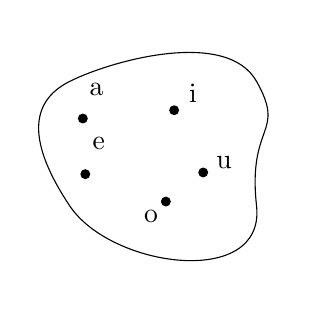
\begin{tikzpicture}[x=0.75pt,y=0.75pt,yscale=-1,xscale=1]
    %uncomment if require: \path (0,300); %set diagram left start at 0, and has height of 300

    %Shape: Polygon Curved [id:ds547955614684159] 
    \draw   (279,111) .. controls (299,101) and (354.6,85.4) .. (369,111) .. controls (383.4,136.6) and (364.6,131) .. (369,171) .. controls (373.4,211) and (299,201) .. (279,171) .. controls (259,141) and (259,121) .. (279,111) -- cycle ;
    %Shape: Circle [id:dp14370499881446686] 
    \draw  [fill={rgb, 255:red, 0; green, 0; blue, 0 }  ,fill opacity=1 ] (283.2,128.9) .. controls (283.2,127.74) and (284.14,126.8) .. (285.3,126.8) .. controls (286.46,126.8) and (287.4,127.74) .. (287.4,128.9) .. controls (287.4,130.06) and (286.46,131) .. (285.3,131) .. controls (284.14,131) and (283.2,130.06) .. (283.2,128.9) -- cycle ;
    %Shape: Circle [id:dp17746710956277556] 
    \draw  [fill={rgb, 255:red, 0; green, 0; blue, 0 }  ,fill opacity=1 ] (284.4,155.7) .. controls (284.4,154.54) and (285.34,153.6) .. (286.5,153.6) .. controls (287.66,153.6) and (288.6,154.54) .. (288.6,155.7) .. controls (288.6,156.86) and (287.66,157.8) .. (286.5,157.8) .. controls (285.34,157.8) and (284.4,156.86) .. (284.4,155.7) -- cycle ;
    %Shape: Circle [id:dp10346397852801814] 
    \draw  [fill={rgb, 255:red, 0; green, 0; blue, 0 }  ,fill opacity=1 ] (323.2,168.9) .. controls (323.2,167.74) and (324.14,166.8) .. (325.3,166.8) .. controls (326.46,166.8) and (327.4,167.74) .. (327.4,168.9) .. controls (327.4,170.06) and (326.46,171) .. (325.3,171) .. controls (324.14,171) and (323.2,170.06) .. (323.2,168.9) -- cycle ;
    %Shape: Circle [id:dp1436157147731828] 
    \draw  [fill={rgb, 255:red, 0; green, 0; blue, 0 }  ,fill opacity=1 ] (327.2,124.9) .. controls (327.2,123.74) and (328.14,122.8) .. (329.3,122.8) .. controls (330.46,122.8) and (331.4,123.74) .. (331.4,124.9) .. controls (331.4,126.06) and (330.46,127) .. (329.3,127) .. controls (328.14,127) and (327.2,126.06) .. (327.2,124.9) -- cycle ;
    %Shape: Circle [id:dp5430919985363672] 
    \draw  [fill={rgb, 255:red, 0; green, 0; blue, 0 }  ,fill opacity=1 ] (341.2,154.9) .. controls (341.2,153.74) and (342.14,152.8) .. (343.3,152.8) .. controls (344.46,152.8) and (345.4,153.74) .. (345.4,154.9) .. controls (345.4,156.06) and (344.46,157) .. (343.3,157) .. controls (342.14,157) and (341.2,156.06) .. (341.2,154.9) -- cycle ;

    % Text Node
    \draw (287.2,111) node [anchor=north west][inner sep=0.75pt]   [align=left] {a};
    % Text Node
    \draw (288.8,137) node [anchor=north west][inner sep=0.75pt]   [align=left] {e};
    % Text Node
    \draw (335.2,111) node [anchor=north west][inner sep=0.75pt]   [align=left] {i};
    % Text Node
    \draw (313.6,171.8) node [anchor=north west][inner sep=0.75pt]   [align=left] {o};
    % Text Node
    \draw (348.4,145.8) node [anchor=north west][inner sep=0.75pt]   [align=left] {u};


    \end{tikzpicture}
    % \includegraphics*[width=\textwidth]{imagefile}

    \caption{元音字母组成的集合}
    \label{元音字母组成的集合}
\end{figure}

\subsection{全称量词 $\forall$ 和存在量词 $\exists$}

在讨论集合中的元素所具有的性质时, 我们常常需要说明这个性质时集合中元素都具有的普遍性质,
还是部分元素才具有的特殊性质. 这就像是你在使用你的操作系统进行文件管理时, 常常需要选中
所有的文件, 或者选中某几个文件来执行某种操作一样. 我们接下来要介绍的全称量词与存在量词,
不严谨地说, 就是在 “选中” 集合中的元素.

使用量词 $\forall$ 和 $\exists$ 的逻辑, 称为谓词逻辑,
含有这些量词的命题称为量化命题.
由于后期还要对谓词逻辑进行更进一步的
讨论, 我们在这里只介绍最常用的结论和最基本的规则.

\subsubsection{全称量词和存在量词}

量词 $\forall$ 表示\textbf{全称量词}, 读作 for every 或者 for all. 符号 $\forall x \in D \left( P(x) \right)$
表示{\kaishu 对于集合 $D$ 中任意给定的元素 $x$, 命题 $P(x)$ 成立}.

量词 $\exists$ 称为\textbf{存在量词}, 读作 there exists. 符号 $\exists x \in D \left( P(x) \right)$
表示{\kaishu 集合 $D$ 中存在一个元素 $x$ 使得命题 $P(x)$ 成立}. 如果使得 $P(x)$ 成立的
$x \in D$ 是唯一的, 那么可以说 $\exists ! x \in D \left( P(x) \right)$.
这就是说, 量词 $\exists$ 强调存在性, 而量词 $\exists!$ 则强调存在性和唯一性.

在 $\forall x \in D$ 与 $\exists x \in D$ 中的集合 $D$ 并不是必须的,
它称为变量的\textbf{论域} (domain of discourse), 也就是命题中的 $x$ 的取值范围.
对于谓词逻辑来说, 指定论述域是非常重要的, 同一个命题在不同的论述域中会有不同的真值.
在不指定论域的时候, 也就是给出形如 $\forall x (P(x))$ 或者 
$\exists x \left(P(x)\right)$ 的量化命题的时候,
那么论域一般是可以根据上下文所确定的. 例如说, 所有地球人的集合很难用一个符号来表达,
那么当它作为论域的时候, 我们就可以省略不写.

我们不加证明地给出如下的量化命题恒等式:
\[ \forall x \left( x \in X \Longrightarrow P(x) \right)
\equiv \forall x \in X \left( P(x) \right),
\quad 
\exists x \left( x \in X \wedge P(x) \right)
\equiv \exists x \in X \left( P(x) \right). \]
这一节的主角是集合, 可不能让它们抢了风头, 我们现在只需要知道关于谓词逻辑的最基本的规则就可以了.
在关于谓词逻辑的进一步讨论中, 我们还会遇到它们.

\begin{example}
    偶数集记作 $2\mathbb{Z}$, {\kaishu 所有偶数 $n$ 都满足 $n$ 模 $2$ 等于 $0$}
    (我们记作 $n \equiv 0 \pmod 2$, 注意与先前的 $n \equiv 1 \pmod 2$ 对比一下看看), 
    可以表示为
    \[ \forall n \in 2\mathbb{Z} \left(
        n \equiv 0 \pmod 2
    \right). \]
\end{example}
\begin{example}
    向量组 $\boldsymbol{a}, \boldsymbol{b}, \boldsymbol{c}$ 线性相关的定义是
    存在一个分量不全为零的数组 $[w_1,w_2,w_2]$, 使得
    向量组 $\boldsymbol{a}, \boldsymbol{b}, \boldsymbol{c}$ 以数组 $[w_1,w_2,w_2]$
    为权的线性组合为零向量. 可以表示为
    \[ \exists [w_1,w_2,w_3] \in \mathbb{R}^3\setminus\left\{\boldsymbol{0}\right\}
    \left(
        w_1\boldsymbol{a} + w_2\boldsymbol{b} + w_3\boldsymbol{c} = \boldsymbol{0}
    \right). \]
\end{example}

\subsubsection{量化命题的否定}

对于全称命题, 只需要构造出一个反例就可以将其否定,
而对于特称命题, 我们则必须要论证整个论述域中的元素都不符合这个命题. 所以,
当我们在否定含有量词的命题的时候, {\kaishu 任意改存在, 存在改任意, 然后把最终的命题 $P(x)$ 取否定}.
\begin{example}
    数列 $\left\{ x_n \right\}$ 有极限 $A$ 的形式逻辑表述为
    \[ \exists A \in \mathbb{R} \forall \varepsilon > 0 \exists N \in \mathbb{N}^+ \forall n>N \left(
        |x_n - A| < \varepsilon
    \right), \]
    它的否定形式是
    \[ \forall A \in \mathbb{R} \exists \varepsilon_0 > 0 \forall N \in \mathbb{N}^+ \exists n_0 > N \left(
        |x_n - A| \geqslant \varepsilon_0
    \right). \]
\end{example}

\subsection{子集}

\begin{definition}[子集]
    如果集合 $A$ 的每个元素都属于集合 $B$, 即
    \[ \forall a \in A \left(
        a \in B
    \right), \]
    则称集合 $A$ 是集合 $B$ 的一个\textbf{子集} (subset). 记作 $A \subset B$.
\end{definition}

容易验证, 对于 $B$ 中任意的元素 $b$, 当然有 $b \in B$, 所以集合 $B$ 是它本身的一个子集.
我们后面还将严格地证明, 空集是任意集合的一个子集. 集合 $B$ 本身与空集 $\varnothing$ 被称为
平凡的子集, 它们往往没有研究的价值, 其余的子集被称为非平凡的子集.

\begin{definition}[真子集]
    如果集合 $A$ 和 $B$ 同时满足以下条件:
    \begin{enumerate}[label={${\arabic*}^\circ$}, itemsep=0pt]
        \item $A \subset B$, 即 $\forall a \in A \left(
            a \in B
        \right)$.
        \item 在 $B$ 中存在元素 $b_0$ 使得 $b_0 \notin A$, 即 $\exists b_0 \in B \left(
            b_0 \notin A
        \right)$.
    \end{enumerate} 
    则称 $A$ 是 $B$ 的一个真子集.
\end{definition}

容易看出, 如果 $A$ 是 $B$ 的真子集, 那么 $A$ 一定是 $B$ 的非平凡的子集, 但反过来则不成立,
即如果 $A$ 是 $B$ 的非平凡的子集, 未必有 $A$ 是 $B$ 的真子集, 这是因为 $A$ 还有可能为
空集.

显然, $A \subset B$ 意味着 $A$ 中所有的元素都是 $B$ 的元素, 如果这时又有 $B \subset A$,
即 $B$ 中所有的元素都是 $A$ 中的元素, 那么其实这时这两个集合包含了完全相同的元素,
我们可以得到 $A=B$, 反过来也是显然成立的 (毕竟一个集合自身可以作为它自己的子集), 
所以我们有如下简单的事实:
\[ A = B \iff A \subset B \wedge B \subset A. \]
因此要证明两个集合相等, 只需要证明它们互为对方的子集, 即它们相互包含. 这是一个简单的事实,
但它却是贯穿整个抽象代数的一个一般的论证方法.

\subsection{幂集}

\begin{definition}[幂集]
    集合 $A$ 的所有子集组成的集合称为集合 $A$ 的\textbf{幂集} (power set),
    记作 $\mathcal{P}(A)$.
\end{definition}
\begin{example}
    集合 $\left\{ 0,1,2 \right\}$ 的幂集是
    \[ \mathcal{P}(\left\{0, 1, 2\right\}) = \left\{
        \varnothing, \left\{ 0 \right\}, \left\{ 1 \right\}, \left\{ 2 \right\},
        \left\{ 0, 1 \right\}, \left\{ 0, 2 \right\}, \left\{
            1,2
        \right\}, \left\{ 0, 1, 2 \right\}
    \right\}. \]
    务必注意空集是任何集合的子集, 且一个集合自身可以作为它自己的子集, 所以它们都属于 
    $\mathcal{P}(\left\{
        0, 1, 2
    \right\})$. 此外, 要注意元素 $a$ 和单元素集合 $\left\{ a \right\}$ 的区别,
    前者是一个元素, 而后者是只含有一个元素的集合.
\end{example}

我们实际上可以通过一种简单的方法来避免在求解有限集合幂集的时候出错, 这种方法就是把集合中的所有元素
按照一定顺序排列, 然后基于在这个子集中是否有这个元素来把集合的每个子集
和一个比特串对应起来. 如果一个元素对应的比特为 $0$, 那么这个元素在这个子集中不出现, 如果
一个元素对应的比特为 $1$, 那么这个元素出现在这个子集中. 具体来讲, 集合 $\left\{0,1,2\right\}$
的所有子集对应的比特串如表 \ref{集合 (0,1,2) 的子集} 所示, 我们只需要把表格最后一列中所有的子集罗列在一起,
就能得到它的幂集.
{\captionof{table}{集合 $\left\{0,1,2\right\}$ 的子集} % 表格标题
\label{集合 (0,1,2) 的子集}
\begin{longtable}{c|ccc|c}
    \toprule
    % 表头
    \textbf{比特串} & \textbf{元素} $2$ & \textbf{元素} $1$ & \textbf{元素} $0$ & \textbf{对应的子集} \\
    \midrule
    \endhead
    \bottomrule
    \endfoot

    % 表格内容
    000 & 0 & 0 & 0 & $\varnothing$ \\ 
    001 & 0 & 0 & 1 & $\left\{ 0 \right\}$ \\
    010 & 0 & 1 & 0 & $\left\{ 1 \right\}$ \\ 
    011 & 0 & 1 & 1 & $\left\{ 0, 1 \right\}$ \\ 
    100 & 1 & 0 & 0 & $\left\{ 2 \right\}$ \\ 
    101 & 1 & 0 & 1 & $\left\{ 0, 2 \right\}$ \\ 
    110 & 1 & 1 & 0 & $\left\{ 1,2 \right\}$ \\ 
    111 & 1 & 1 & 1 & $\left\{ 0, 1, 2 \right\}$ \\
\end{longtable}}

\begin{example}
    由于空集只有一个子集, 即空集自身, 所以 $\mathcal{P}(\varnothing) = \left\{
        \varnothing
    \right\}$. 要注意 $\left\{ \varnothing \right\}$ 与 $\varnothing$ 是两个不一样的
    概念, 前者是单元素集合, 其元素为空集. 而后者是一个集合, 不过它不含任何元素.
\end{example}

\subsection{交集、并集与差集}

\begin{figure}[H]
    \centering
    % 图的内容
    \begin{minipage}{0.3\textwidth}
        \centering
        \tikzset{every picture/.style={line width=0.75pt}} %set default line width to 0.75pt        

        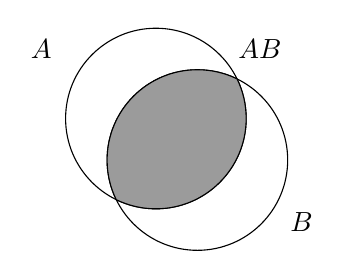
\begin{tikzpicture}[x=0.75pt,y=0.75pt,yscale=-1,xscale=1]
        %uncomment if require: \path (0,300); %set diagram left start at 0, and has height of 300

        %Shape: Circle [id:dp9416059956393634] 
        \draw   (178,124.5) .. controls (178,100.48) and (197.48,81) .. (221.5,81) .. controls (245.52,81) and (265,100.48) .. (265,124.5) .. controls (265,148.52) and (245.52,168) .. (221.5,168) .. controls (197.48,168) and (178,148.52) .. (178,124.5) -- cycle ;
        %Shape: Circle [id:dp8452481279219075] 
        \draw   (198,144.5) .. controls (198,120.48) and (217.48,101) .. (241.5,101) .. controls (265.52,101) and (285,120.48) .. (285,144.5) .. controls (285,168.52) and (265.52,188) .. (241.5,188) .. controls (217.48,188) and (198,168.52) .. (198,144.5) -- cycle ;

        %Shape: Path Data [id:dp10855579595172649] 
        \draw  [fill={rgb, 255:red, 155; green, 155; blue, 155 }  ,fill opacity=1 ] (241.5,101) .. controls (248.35,101) and (254.83,102.58) .. (260.6,105.4) .. controls (263.42,111.17) and (265,117.65) .. (265,124.5) .. controls (265,148.52) and (245.52,168) .. (221.5,168) .. controls (214.65,168) and (208.17,166.42) .. (202.4,163.6) .. controls (199.58,157.83) and (198,151.35) .. (198,144.5) .. controls (198,120.48) and (217.48,101) .. (241.5,101) -- cycle ;

        % Text Node
        \draw (160,85.4) node [anchor=north west][inner sep=0.75pt]    {$A$};
        % Text Node
        \draw (285,168.4) node [anchor=north west][inner sep=0.75pt]    {$B$};
        % Text Node
        \draw (260,85.4) node [anchor=north west][inner sep=0.75pt]    {$AB$};


        \end{tikzpicture}
        \subcaption{交集}
    \end{minipage}
    \begin{minipage}{0.3\textwidth}
        \centering
        \tikzset{every picture/.style={line width=0.75pt}} %set default line width to 0.75pt        

        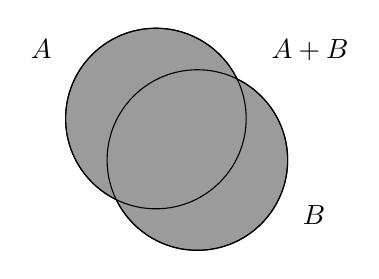
\begin{tikzpicture}[x=0.75pt,y=0.75pt,yscale=-1,xscale=1]
        %uncomment if require: \path (0,300); %set diagram left start at 0, and has height of 300

        %Shape: Path Data [id:dp06887185201661039] 
        \draw  [fill={rgb, 255:red, 155; green, 155; blue, 155 }  ,fill opacity=1 ] (241.5,101) .. controls (258.67,101) and (273.52,110.95) .. (280.6,125.4) .. controls (282.12,126.15) and (283.59,126.98) .. (285,127.89) .. controls (297.03,135.63) and (305,149.13) .. (305,164.5) .. controls (305,188.52) and (285.52,208) .. (261.5,208) .. controls (254.29,208) and (247.49,206.25) .. (241.5,203.14) .. controls (233.23,198.85) and (226.51,191.98) .. (222.4,183.6) .. controls (207.95,176.52) and (198,161.67) .. (198,144.5) .. controls (198,120.48) and (217.48,101) .. (241.5,101) -- cycle ;
        %Shape: Circle [id:dp326406041975832] 
        \draw   (198,144.5) .. controls (198,120.48) and (217.48,101) .. (241.5,101) .. controls (265.52,101) and (285,120.48) .. (285,144.5) .. controls (285,168.52) and (265.52,188) .. (241.5,188) .. controls (217.48,188) and (198,168.52) .. (198,144.5) -- cycle ;
        %Shape: Circle [id:dp521202262674819] 
        \draw   (218,164.5) .. controls (218,140.48) and (237.48,121) .. (261.5,121) .. controls (285.52,121) and (305,140.48) .. (305,164.5) .. controls (305,188.52) and (285.52,208) .. (261.5,208) .. controls (237.48,208) and (218,188.52) .. (218,164.5) -- cycle ;


        % Text Node
        \draw (180,105.4) node [anchor=north west][inner sep=0.75pt]    {$A$};
        % Text Node
        \draw (311,185.4) node [anchor=north west][inner sep=0.75pt]    {$B$};
        % Text Node
        \draw (296,105.4) node [anchor=north west][inner sep=0.75pt]    {$A+B$};


        \end{tikzpicture}
        \subcaption{并集}
    \end{minipage}
    \begin{minipage}{0.3\textwidth}
        \centering




        \tikzset{every picture/.style={line width=0.75pt}} %set default line width to 0.75pt        

        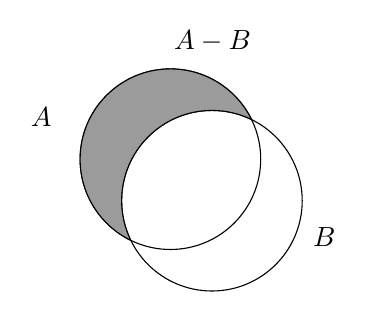
\begin{tikzpicture}[x=0.75pt,y=0.75pt,yscale=-1,xscale=1]
        %uncomment if require: \path (0,300); %set diagram left start at 0, and has height of 300
        
        %Shape: Circle [id:dp8889061377956761] 
        \draw   (198,144.5) .. controls (198,120.48) and (217.48,101) .. (241.5,101) .. controls (265.52,101) and (285,120.48) .. (285,144.5) .. controls (285,168.52) and (265.52,188) .. (241.5,188) .. controls (217.48,188) and (198,168.52) .. (198,144.5) -- cycle ;
        %Shape: Circle [id:dp897868618118875] 
        \draw   (218,164.5) .. controls (218,140.48) and (237.48,121) .. (261.5,121) .. controls (285.52,121) and (305,140.48) .. (305,164.5) .. controls (305,188.52) and (285.52,208) .. (261.5,208) .. controls (237.48,208) and (218,188.52) .. (218,164.5) -- cycle ;
        
        %Shape: Path Data [id:dp27631101420474025] 
        \draw  [fill={rgb, 255:red, 155; green, 155; blue, 155 }  ,fill opacity=1 ] (241.5,101) .. controls (258.67,101) and (273.52,110.95) .. (280.6,125.4) .. controls (274.83,122.58) and (268.35,121) .. (261.5,121) .. controls (237.48,121) and (218,140.48) .. (218,164.5) .. controls (218,171.35) and (219.58,177.83) .. (222.4,183.6) .. controls (207.95,176.52) and (198,161.67) .. (198,144.5) .. controls (198,120.48) and (217.48,101) .. (241.5,101) -- cycle ;
        
        % Text Node
        \draw (173,118.4) node [anchor=north west][inner sep=0.75pt]    {$A$};
        % Text Node
        \draw (309,176.4) node [anchor=north west][inner sep=0.75pt]    {$B$};
        % Text Node
        \draw (242,81.4) node [anchor=north west][inner sep=0.75pt]    {$A-B$};
        
        
        \end{tikzpicture}
        \subcaption{差集}
    \end{minipage}
    % \includegraphics*[width=\textwidth]{imagefile}

    \caption{交集、并集与补集}
    \label{交集、并集与补集}
\end{figure}

\begin{definition}[交集]
    由集合 $A$ 和集合 $B$ 的所有公共元素作成的集合
    \[ A \cap B := \left\{ x | x \in A \wedge x \in B \right\} \]
    称为 $A$ 与 $B$ 的\textbf{交集} (intersetcion), 记作 $A \cap B$.
    集合的交集也称为集合的积, 有时也像代数积一样将其写作 $AB$.
\end{definition}

\begin{definition}[并集]
    由属于集合 $A$ 或者属于集合 $B$ 的元素作成的集合
    \[ A \cup B := \left\{ x | x \in A \vee x \in B \right\} \]
    称为 $A$ 与 $B$ 的\textbf{并集} (union), 记作 $A \cup B$.
    集合的并集也称为集合的和, 有时也像代数和一样将其写作 $A + B$.
\end{definition}

正如先前所述, 符号 $\wedge$ 表示命题的合取, 即它左右两边的命题同时成立.
符号 $\vee$ 表示命题的析取, 它表示它左右两边的命题至少有一个成立.

\begin{definition}[差集]
    由属于集合 $A$ 但不属于集合 $B$ 的元素作成的集合
    \[ A \setminus B := \left\{ x \in A | x \notin B \right\} \]
    称为 $A$ 与 $B$ 的\textbf{差集} (set difference), 记作 $A \setminus B$.
    有时也像代数差一样将其写作 $A-B$.
\end{definition}

\begin{definition}[补集]
    设 $\varOmega$ 是一个集合, 集合 $A$ 是它的子集. 集合
    \[ \varOmega \setminus A = \left\{ x \in \varOmega | x \notin A \right\} \]
    称为 $A$ 在 $\Omega$ 中的\textbf{补集} (complement), 记作 $\complement_\varOmega A$.
    或者 $\bar A$.
\end{definition}

容易验证的是, 从集合 $A$ 中排除掉集合 $B$ 中的元素, 本质上是在排除集合 $A$ 与集合 $B$
的交集中的元素 (试想, 你该怎么开出一个本来就不属于你的公司的员工), 
而对于给定的论域 $\Omega$ 来说, 别忘了它是一个确定的集合, 而不是 “宇宙中所有事物组成的全体”, 
假设 $A,B$ 都是 $\varOmega$ 的子集, $x \in A$ 且 $x \notin B$, 实际上意味着
$x \in A$ 且 $x \in \bar B$. 因此我们有以下
公式, 它在集合论和概率论中非常重要:
\[ \boxed{A \setminus B = A - B = A-AB = A\bar B.} \]

\begin{figure}[H]
    \centering
    % 图的内容
    \begin{minipage}{0.45\textwidth}
        \centering
        \tikzset{every picture/.style={line width=0.75pt}} %set default line width to 0.75pt        

        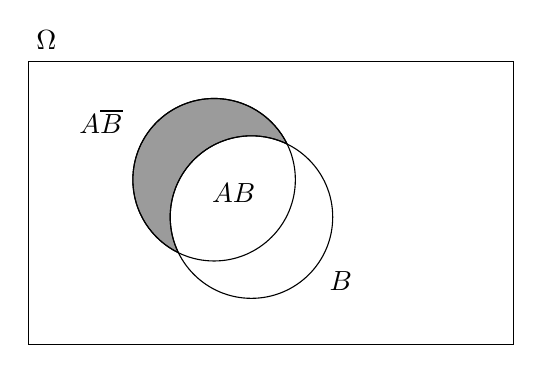
\begin{tikzpicture}[x=0.75pt,y=0.75pt,yscale=-0.9,xscale=0.9]
        %uncomment if require: \path (0,300); %set diagram left start at 0, and has height of 300

        %Shape: Rectangle [id:dp9464405787386964] 
        \draw   (142,81) -- (402,81) -- (402,232.5) -- (142,232.5) -- cycle ;
        %Shape: Path Data [id:dp5798883752780631] 
        \draw  [fill={rgb, 255:red, 155; green, 155; blue, 155 }  ,fill opacity=1 ] (241.5,101) .. controls (258.67,101) and (273.52,110.95) .. (280.6,125.4) .. controls (274.83,122.58) and (268.35,121) .. (261.5,121) .. controls (237.48,121) and (218,140.48) .. (218,164.5) .. controls (218,171.35) and (219.58,177.83) .. (222.4,183.6) .. controls (207.95,176.52) and (198,161.67) .. (198,144.5) .. controls (198,120.48) and (217.48,101) .. (241.5,101) -- cycle ;
        %Shape: Circle [id:dp31127546551589236] 
        \draw   (198,144.5) .. controls (198,120.48) and (217.48,101) .. (241.5,101) .. controls (265.52,101) and (285,120.48) .. (285,144.5) .. controls (285,168.52) and (265.52,188) .. (241.5,188) .. controls (217.48,188) and (198,168.52) .. (198,144.5) -- cycle ;
        %Shape: Circle [id:dp4958876631095299] 
        \draw   (218,164.5) .. controls (218,140.48) and (237.48,121) .. (261.5,121) .. controls (285.52,121) and (305,140.48) .. (305,164.5) .. controls (305,188.52) and (285.52,208) .. (261.5,208) .. controls (237.48,208) and (218,188.52) .. (218,164.5) -- cycle ;


        % Text Node
        \draw (168,105.4) node [anchor=north west][inner sep=0.75pt]    {$A\overline{B}$};
        % Text Node
        \draw (302,192.4) node [anchor=north west][inner sep=0.75pt]    {$B$};
        % Text Node
        \draw (239,145.4) node [anchor=north west][inner sep=0.75pt]    {$AB$};
        % Text Node
        \draw (145,63.4) node [anchor=north west][inner sep=0.75pt]    {$\si{\ohm}$};


        \end{tikzpicture}
        \subcaption{差集}
    \end{minipage}
    \begin{minipage}{0.45\textwidth}
        \centering

        \tikzset{every picture/.style={line width=0.75pt}} %set default line width to 0.75pt        

        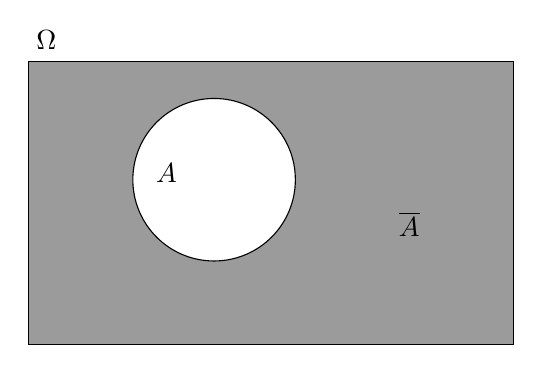
\begin{tikzpicture}[x=0.75pt,y=0.75pt,yscale=-0.9,xscale=0.9]
        %uncomment if require: \path (0,300); %set diagram left start at 0, and has height of 300

        %Shape: Rectangle [id:dp39855013718260934] 
        \draw  [fill={rgb, 255:red, 155; green, 155; blue, 155 }  ,fill opacity=1 ] (142,81) -- (402,81) -- (402,232.5) -- (142,232.5) -- cycle ;
        %Shape: Circle [id:dp28915123578730806] 
        \draw  [fill={rgb, 255:red, 255; green, 255; blue, 255 }  ,fill opacity=1 ] (198,144.5) .. controls (198,120.48) and (217.48,101) .. (241.5,101) .. controls (265.52,101) and (285,120.48) .. (285,144.5) .. controls (285,168.52) and (265.52,188) .. (241.5,188) .. controls (217.48,188) and (198,168.52) .. (198,144.5) -- cycle ;

        % Text Node
        \draw (209,134.4) node [anchor=north west][inner sep=0.75pt]    {$A$};
        % Text Node
        \draw (339,160.4) node [anchor=north west][inner sep=0.75pt]    {$\overline{A}$};
        % Text Node
        \draw (145,63.4) node [anchor=north west][inner sep=0.75pt]    {$\si{\ohm}$};


        \end{tikzpicture}
        \subcaption{补集}
    \end{minipage}
    % \includegraphics*[width=\textwidth]{imagefile}

    \caption{差集与补集}
    \label{差集与补集}
\end{figure}

\subsection{集合恒等式}

集合的交、并、差、补都是集合的运算 (注意, 不能说是定义在集合的集合上的运算, 因为 “所有集合的
集合” 这个东西就像 “宇宙中所有事物组成的全体” 一样是会引起悖论的). 它们满足一些恒等式,
我们以对这些恒等式的罗列来结束本节, 如表 \ref{集合恒等式} 所示, 这些恒等式的证明都是明显的, 
你可以用 $A = B \iff A \subset B \wedge B \subset A$ 来简单地证明它们, 在此不再赘述.
在以下的所有讨论中, 假设 $\varOmega$ 是一个给定的集合, $A, B$ 为其子集.

注意到我们在书写这些性质的时候才用了类似代数和、代数积的写法, 不难发现, 空集 $\varnothing$
在集合的加法 (这就是并集) 和乘法 (这就是交集) 中发挥着加法单位元和乘法零元的作用. 而论域
$\varOmega$ 在集合的加法和乘法中发挥着乘法单位元的作用. 在后续学习布尔代数时,
读者应注意比较学习集合恒等式、命题等价式与布尔恒等式的联系.

{\captionof{table}{集合恒等式} % 表格标题
\label{集合恒等式}
\begin{longtable}{p{0.33\textwidth}|c||p{0.33\textwidth}|c}
    \toprule
    % 表头
    \textbf{恒等式} & \textbf{名称} & \textbf{恒等式} & \textbf{名称} \\ 
    \midrule
    \endhead
    \bottomrule
    \endfoot

    % 表格内容
    $\overline{\left(\bar A\right)} = A$ & 双重补律 & $A + BC = (A+B)(A+C)$
        
    $A(B+C) = AB+AC$& 分配律\\
    \midrule
    $A \cup A = A+A = A$ 

    $A \cap A = AA = A$ & 幂等律 & $\overline{AB} = \bar A + \bar B$

    $\overline{A + B}=\bar A\bar B$ & De Morgan 律 \\ 
    \midrule
    $A \cup \varnothing = A+\varnothing = A$

    $A \cap \varOmega = A\varOmega = A$ & 同一律 & $A + AB=A$

    $A(A+B) = A$ & 吸收律 \\
    \midrule 
    $A \cup \varOmega = A + \varOmega = \varOmega$ 

    $A \cap \varnothing = A \varnothing = \varnothing$ & 支配律 & $A + \bar A = \varOmega$ & $\varOmega$ 的性质 \\ 
    \midrule 
    $A + B = B + A$

    $AB = BA$ & 交换律 & $A\bar A = \varnothing$ 
    
    $\varnothing$ 与 $\varOmega$ 的性质统称为 “互补律” & $\varnothing$ 的性质 \\ 
    \midrule 
    $A + (B + C) = (A + B) + C$ 

    $A(BC) = (AB)C$ & 结合律 & & \\ 
\end{longtable}}

\newpage
\subsection{ZFC 公理系统}

细心的读者可能会注意到我们在给出集合的概念时并没有使用表示定义的 \lstinline|definition|
环境. 事实上, 将集合描述为对象的聚集最先是由德国
数学家 George Cantor\footnote{
    乔治·康托尔 (Georg Cantor, 1845—1918) 是19世纪末至20世纪初德国著名的数学家, 他被公认为集合论的创始人之一, 同时也是无穷集合理论的奠基人.  Cantor 的贡献在于他对无限集合的研究和理解, 这使得数学界对于无限的概念有了更深入的认识. 他提出了著名的 Cantor 定理, 证明了有限集合和无限集合之间存在着不同的势. 这一理论为数学奠定了更深的基础, 并推动了数学在这个领域的发展.  Cantor 的研究不仅在数学上产生了深远的影响, 而且在哲学上也引发了许多思考. 他的工作促进了数学思维的革新, 并启发了许多后来的数学家和哲学家. 然而,  Cantor 的工作也引起了不少争议和批评, 因为他的理论挑战了传统的数学观念和直觉. 尽管如此,  Cantor 的贡献被广泛认可, 他被视为现代数学中最伟大的思想家之一, 他的工作对于数学和哲学的发展都具有不可估量的价值. 
} 提出的, 英国哲学家 Bertrand Russell\footnote{
    伯特兰·罗素 (Bertrand Russell, 1872—1970) 是一位著名的英国哲学家、逻辑学家、数学家和社会评论家, 
    他在各个领域都做出了重大贡献. 出生于 1872 年的 Russell 以逻辑和分析哲学而闻名, 特别是他与阿尔弗雷德·北·怀特海德 (Alfred North Whitehead) 合作的重要著作《数学原理》 (Principia Mathematica) , 旨在建立数学的逻辑基础.  Russell 在逻辑方面的贡献包括他对类型理论的发展以及他对逻辑悖论的研究, 如著名的 Russell 悖论, 它质疑了集合论的基础. 除了对逻辑和数学的贡献外,  Russell 在哲学上也是一位有影响力的人物, 主张经验主义、逻辑分析和批判性思维的重要性. 他的哲学著作涵盖了伦理学、政治学、宗教学和现实的本质等广泛主题.  Russell 是战争和帝国主义的坚决批评者, 在其一生中积极参与政治和社会活动. 1950年, 他因广泛的文学作品和对人类思想进步的贡献而被授予诺贝尔文学奖.  Russell 的遗产继续影响着当代哲学、逻辑学和社会评论, 并且他仍然是20世纪最重要的思想家之一. 
} 在 1902 年证实了由{\kaishu 集合的直觉定义}以及
{\kaishu 无论什么性质都存在一个恰好由该性质的对象组成的集合}这种直觉概念的使用将导致
\textbf{悖论} (paradox).
因此必须要限制集合形成的可能性, 关于从公理出发构造集合论的学说称为公理化集合论,
我们接下来要介绍的就是著名的 \textbf{ZFC 公理系统} (Zermelo-Fraenkel set theory with the Axiom of Choice).

\subsubsection{集合形成的可能性}

下述的若干公理建立了一个公理系统来描述称为\textbf{集合} (set) 的数学对象的性质. 我们首先
罗列这些公理, 然后再做出解释并给出它们的形式逻辑表述. 在这一小节中我们将只考虑集合, 这是因为
由各种元素组成的集合也可以作为其他集合的元素, 有一句话说得非常形象, {\kaishu 在这个世界上除了集合之外
什么都没有}. 我们在这一小节中, 按照逻辑学家们的习惯,
也用小写字母表示集合.

\setcounter{axiom}{0}
\begin{axiom}[外延公理]
    集合 $A$ 与集合 $B$ 相等, 当且仅当它们所具有的各元素是相同的.
\end{axiom}
\begin{axiom}[分离公理]
    任何集合 $A$ 和性质 $P$ 都对应一个集合 $B$, 
    其元素是且仅是集合 $A$ 中具有性质 $P$ 的各元素.
\end{axiom}





\begin{axiom}[并集公理]
    对于集合的任何集合 $\mathscr{A}$ (即集合族 $\mathscr{A}$), 存在一个被称为
    $\mathscr{A}$ 的并集的集合 $\cup \mathscr{A}$, 其元素是且仅是 $\mathscr{A}$
    中各个元素所包含的那些元素.
\end{axiom}

% \begin{example}
%     根据并集公理和分离公理, 我们可以给出集合族 $\mathscr{A}$ 的交集 $\cap \mathscr{A}$
%     的定义, 并集概念的核心是并集中的元素属于集合族中的每一个集合, 因此 
%     $\cap \mathscr{A} \xlongequal{\mathrm{def}} \left\{ x \in \cup 
%     \mathscr{A} | \forall A \in \mathscr{A} (x \in A) \right\}$.
% \end{example}

\begin{axiom}[配对公理]
    对于任何集合 $X$ 和集合 $Y$, 存在一个集合 $Z$, 其元素是且仅是 $X$ 和 $Y$.
    % 将该集合记作 $\left\{ X,Y \right\}$, 
    % 称为集合 $X,Y$ 的{\normalfont\bfseries 无序偶}.
\end{axiom}

\begin{axiom}[子集之集公理]
    对于任意给定的集合 $A$, 存在一个集合 $\mathscr{P}(A)$, 使得 $\mathscr{P}(A)$
    中的元素是且仅是 $A$ 的各子集. 
    % $\mathscr{P}(A) = \left\{ X | X \subset A \right\}$.
\end{axiom}

% \begin{example}
%     现在我们来回答为什么要按照定义 \ref{def: 二元关系} 的方式来定义二元关系.
%     T.B.C. \label{TBC}
% \end{example}

公理 $1 \sim 5$ 限制了形成新集合的可能性,
我们接下来简单地解释一下这些公理, 然后展示这些公理的一些最简单的推论.

外延公理表示, {\kaishu 我们只关心 “集合” 这一对象是否具有给定元素, 而不关心它的一切其他性质}.
即我们要验证 $A = B$, 只需要验证 $\forall x \left( x \in A \equiv x \in B \right)$.
它的形式逻辑表示为
\[ \forall x \forall y \forall z \left( \quad
    ((z \in x) \equiv (z \in y)) \,\, \equiv \,\, x=y
\quad \right). \]
汗流浃背了吧老兄, 没关系, 我也汗流浃背, 不过好在这一节的内容不是考试内容, 所以我们只需要做一点
简单的了解即可. 简单的解释一下吧, 这里的 $x$ 和 $y$ 是两个集合, 而 $z$ 实际上可以被理解为
是 $x$ 与 $y$ 中的元素. 这个量化命题是在说, 
{\kaishu 集合 $x$ 与集合 $y$ 相等 (即 $x=y$)} 当且仅当 {\kaishu $z \in x$ 与 $z \in y$
是逻辑等价的, 即 $(z \in x) \equiv (z \in y)$}, 这符合外延公理对集合的描述.
注意到我特地使用了空格来划分这个量化命题的结构, 如果我不这么做的话, 你可能会更抓狂,
请看:
\[ \forall x \forall y \forall z \left(
((z \in x) \equiv (z \in y)) \equiv x=y
\right), \]
我看到它的第一眼甚至分辨不出 $=$ 和 $\equiv$ 的区别, 当场血压就高了. 不过呢你大可放心,
我已经为你把后面的每一个复杂的逻辑命题都划分好结构了 (除非我想整蛊你一下), 
你看我贴不贴心啊, 是不是应该找个机会好好奖励我一下呢小哥哥/小姐姐/大哥哥/大姐姐 $\left.:\right)$

分离公理说的是, 如果 $A$ 是一个集合, $P(x)$ 是一个性质 (或者说命题),
那么 $B = \left\{ x | x \in A \wedge P(x) \right\}$ 也是一个集合.
它给我们提供了从一些集合中分离出由具有某种性质的元素组成的子集的方法.

并集公理的一个更常见的表述是 {\kaishu 由集合族中诸集合的元素组成的集合是存在的}, 即集合的
并集是一个集合. 它的形式逻辑表述是
\[ \forall x \exists y \forall z \left( \quad
    z \in y \,\,\equiv\,\, \exists w \left(
        z \in w \wedge w \in x
    \right) \quad 
\right), \]
这就是说, {\kaishu 任意的集合族 $x$ 都存在它的并集 $y$, 一个元素 $z$ 属于这个并集当且仅当在集合族
$x$ 中存在集合 $w$ 使得 $z \in w$}. 于是我们验证了这个量化命题确实是并集公理的一个有效的
表述.

配对公理说的是对于任意的集合 $X$ 和集合 $Y$ 都存在一个集合 $Z = \left\{ X,Y \right\}$,
它称为集合 $X$ 与 $Y$ 的无序偶. 如果 $X=Y$, 则 $Z = \left\{ X \right\}$ 就是一个
单元素集合. 配对公理的形式逻辑表述为
\[ \forall x \forall y \exists z \forall v \left(\quad
    v \in z \,\, \equiv \,\, v = x \vee v = y
\quad\right), \]
翻译一下, {\kaishu 对于任意的集合 $x$ 和集合 $y$ 都存在一个集合 $z$, 元素 $v$ 属于集合 $z$
当且仅当元素 $v$ 就是集合 $x$ 或者元素 $v$ 就是集合 $y$}. 因此集合 $z$ 确实是集合 $x,y$
所确定的无序偶, 这个量化命题确实给出了配对公理的一个有效的表述.

子集之集公理说明了一个集合的幂集是存在的, 它的形式逻辑表述为
\[ \forall x \exists y \forall z \left(
    \quad
    z \in y \,\, \equiv\,\, 
    \forall u \left(
        u \in z \Rightarrow u \in x
    \right)
    \quad
\right), \]
其中的符号 $\Rightarrow$ 表示 $u \in z \to u \in x$ 是永真式. 说人话就是, 任给一个
集合 $x$ 都存在它的幂集 $y$ 使得元素 $z$ 属于幂集 $y$ 当且仅当 $z$ 是 $x$ 的子集.
而 $z$ 是 $x$ 的子集就是说, 任意的元素 $u$ 只要属于 $z$ 就一定属于 $x$, 即
$z \subset x \,\, \equiv \,\, \forall u \left(
    u \in z \Longrightarrow u \in x
\right)$. 所以集合 $y$ 确实是 $x$ 的所有子集的集合, 这一量化命题确实是子集之集公理的
有效表述 (其实慢慢读、慢慢理解再仔细分析, 然后看出命题的结构的话, 也没有那么难, 对吧).

接下来, 我们基于公理 1 $\sim$ 公理 5 来总结一下集合形成的各种可能性. 首先我们需要讨论
空集、并集和交集的存在性.

\begin{example}
    试证明 {\kaishu $\forall A \left( \varnothing \subset A \right)$, 即空集是任何集合的
    子集}.
    \begin{proof}
        分离公理在一些数学结构中是很常用的, 我们需要从一个集合 $A$ 中分离出具有性质
        $P$ 的元素来. 显然, 在这个问题中, 设 $X$ 是一个集合, 那么我们能够分离出它的
        空子集 $\varnothing_X = \left\{ x \in X | x \ne x \right\}$ 来.
        设 $Y$ 是另一个任意给定的集, 有 $\varnothing_Y = \left\{ y \in Y |
        y \ne y \right\}$, 根据外延公理, $\varnothing_X = \varnothing_Y$.
        由于我们的 $X,Y$ 都是任意给定的集合, 这就是说, 空集是唯一的, 我们用 $\varnothing$
        来表示空集, 并且, 任何集合都有空子集.
    \end{proof}
\end{example}
\begin{example}
    我们可以用分离公理来理解差集运算, 设 $A,B$ 是两个集合, $A \setminus B
    \xlongequal{\mathrm{def}} \left\{ x \in A | x \notin B \right\}$,
    显然这里的 $A$ 是一个集合, 而 $x \notin B$ 是一个性质, 它们总是能够确定
    这样的集合 $A \setminus B$. 特别的, 如果 $\varOmega$ 是一个集合, $A \subset \varOmega$
    是它的一个子集, 那么 $\bar A$ 也是一个集合.
\end{example}
\begin{example}
    并集公理说明了并集的存在性, 而结合并集公理和分离公里, 就可以定义集合族 $\mathscr{A}$ 的交集
    \[ \cap \mathscr{A} := \left\{
        x \in \cup \mathscr{A} | \forall X \in \mathscr{A} \left( x \in X \right)
    \right\}, \]
    我们在这里使用 $\forall X \in \mathscr{A}(x \in X)$ 来代替了 $\forall X \left( X \in \mathscr{A} \Rightarrow x \in X \right)$.
    显然这里的 $\forall X \in \mathscr{A} \left( x \in X \right)$ 就是这样的
    一个性质, 它从 $\cup\mathscr{A}$ 中分离出了 $\cap\mathscr{A}$.
\end{example}

\begin{example}
    配对公理给出了无序偶 $\left\{ X,Y \right\}$, 我们可以进一步地定义序偶
    $(X,Y) = \left\{ \left\{X\right\}, \left( X,Y \right) \right\}$.
    由此我们可以递归地定义 $n$ 元组为 $\left( (a_1, a_2, \cdots, a_{n-1}), a_n \right)$.
    于是基于配对公理和子集之集公理我们可以定义集合 $X$ 与 $Y$ 的 Descartes 积为
    \[ X \times Y := \left\{p \in \mathcal{P}\left(
        \mathcal{P}\left(
            X \cup Y
        \right)
    \right) | p = (x, y) \wedge x \in X \wedge y \in Y \right\}. \]
\end{example}

综上所述, 在 ZFC 公理系统中, 一个集合的形成主要是通过以下罗列的几种方式, 它们实际上都是我们
所熟识的集合运算:
\begin{itemize}[itemsep=0pt]
    \item 基于分离公理从集合中分离出具有某种特性的元素组成的子集;
    \item 集合的并集、交集和差集、集合的幂集;
    \item 集合的 Descartes 积.
\end{itemize}

\subsubsection{后继集、归纳集和无穷公理}

为了表述下面的公理, 我们需要给定后继集和归纳集的概念.
设 $X$ 是一个集合, 集合 $X \cup \left\{ X \right\}$ 称为 $X$ 的\textbf{后继集},
即在 $X$ 中补充一个单元素集合 $\left\{ X \right\}$. 集合 $X$ 的后继集记作
$X^+$.
假设 $X$ 是一个集合, 如果 $X$ 包含空集以及自身任何一个元素的后继集, 则称 $X$
是一个归纳集.


\begin{axiom}[无穷公理]
    归纳集存在.
\end{axiom}

我们接下来建立无穷公理的形式逻辑表述. 这一次构造量化命题的难度稍微有些大, 所以我们分步骤地
构造这个量化命题. 我们知道, 归纳集是包含空集以及其自身任何一个元素的后继集的集合, 这就是说,
我们需要构造一个量化命题, 说明这样的集合 $x$ 是存在的, 它同时满足以下两个条件:
\begin{enumerate}[label={${\arabic*}^\circ$}, itemsep=0pt]
    \item $\varnothing \in x$,
    \item $\forall w \left( w \in x \Rightarrow w^+ \in x \right)$.
\end{enumerate}
接下来让我们仅用逻辑连接词、$\in$ 和 $\equiv$ 来把这个命题 “翻译出来”.
让我们首先来看 $\varnothing \in x$. 要说明 $\varphi \in x$, 只需要说明任何的没有元素的
集合都属于 $x$, 这就是说, 假设 $y$ 是一个集合, 那么
\[ y = \varnothing \,\,\equiv\,\, \nexists z(z \in y), \]
于是只要集合 $y$ 没有元素, 是空集, $y$ 就属于 $x$:
\[ \varnothing \in x \,\,\equiv\,\, \forall y \left( \quad \nexists z(z \in y)
\Rightarrow y \in x \quad \right). \]
接下来我们来讨论 $x$ 中任意的元素 $w$ 的后继集 $w^+$ 也属于 $x$, 我们知道,
$w^+ = w \cup \left\{w\right\}$, 所以任意给定的元素 $v \in w^+$ 当且仅当 $v \in w$
或者 $v = w$. 这就是说, 集合 $u$ 是 $w$ 的后继集当且仅当
\[ \forall v \left( \quad v \in u \,\,\equiv\,\, v=w \vee v \in w \quad \right) \]
$w^+ \in x$, 就是说满足上述条件的集合 $u$ 都属于 $x$, 即
\[ \forall w \left(
    w \in x \Rightarrow \forall u \left(
        \forall v \left( \quad v \in u \,\,\equiv\,\, v=w \vee v \in w \quad \right)
        \Rightarrow u \in x
    \right)
\right) \]
于是我们成功的翻译了这两个命题, 把他们用最基本的逻辑连接词和 $\in$、$\equiv$ 符号表达出来了.
接下来只需要取它们两个命题的合取, 就能得到无穷公理的形式逻辑表示:
\[ \exists x \left(
    \forall y \left(
        \lnot \exists z \left( z \in y \right)
        \Rightarrow y \in x
    \right) \wedge \forall w \left(
        w \in x \Rightarrow \forall u \left(
            \forall v \left(
                v \in u \equiv \left(
                    v = w \vee v \in w
                \right) 
            \right)
            \Rightarrow u \in x
        \right)
    \right)
\right). \]
累吗? 我也累了, 这个故事告诉我们随着命题复杂程度的提高, 基本的逻辑符号似乎有点不够用了,
所以剩下的几个公理我们不再给出最基本的量化命题表述,
转而采用更有效率的量化命题表述方式.

\begin{example}
    根据无穷公理和公理 $1 \sim 4$, 我们可以建立自然数集 $\mathbb{N}_0$ 的 von 
    Neumann 方案. 我们把自然数集 $\mathbb{N}_0$ 定义为各归纳集的交集, 即最小归纳集.
    $\mathbb{N}_0$ 的元素是集合
    \[ \varnothing, \varnothing^+, \left( \varnothing^+ \right)^+, \]
    其中, $\varnothing^+ = \varnothing \cup \left\{ \varnothing \right\}
    = \left\{ \varnothing \right\}$, 而 $\left\{ \varnothing \right\}^+
    = \left\{ \varnothing \right\} \cup \left\{ 
        \left\{ \varnothing \right\}
    \right\}$. 这些集合就是我们用符号 $0,1,2,\cdots$ 表示的并称之为自然数的
    数学对象的模型.
\end{example}

\subsubsection{替换公理与选择公理}

不同于分离公理只能构造出集合 $X$ 的子集, 替换公理给我们提供了从已知集合和已知命题构造
可以与已知集合不同的集合的方式. 不过我们在建立分析学时不会用到这个公理.

\begin{axiom}[替换公理]
    设 $\mathcal{F}(x,y)$ 是以下命题: 对于集合 $X$ 中的任何元素 $x_0$, 存在唯一的对象
    $y_0$ 使得 $F(x_0, y_0)$ 成立. 那么, 满足以下条件的 $y$ 组成一个集合:
    存在 $x \in X$ 使得 $\mathcal{F}(x,y)$ 成立.
\end{axiom}

这就是说, 如果
\[ \forall x_0 \in X \exists ! y_0  (\mathcal{F}(x_0, y_0)) ,\]
那么
\[ \left\{ y | \exists x \in X  (\mathcal{F}(x,y))  \right\} \]
是一个集合. 因此替换公理可以表述为
\[ \forall X \left( 
    \forall x_0 \in X\exists ! y_0 (\mathcal{F}(x_0, y_0))
    \quad \Longrightarrow \quad 
    \exists Y \forall y \left(  y \in Y \Leftrightarrow
    \exists x \in X (\mathcal{F}(x,y)) \right)
\right) \]
为了不使得命题过于复杂, 我们选择保留唯一性量词 $\exists ! y_0$.

公理 1 $\sim$ 公理 7 被称为 Zermelo-Fraenkel 公理系统,
不过通常我们还补充如下的选择公理, 因为它在分析学中是很常用的.

\begin{axiom}[选择公理]
    对于任何由互不相交非空集合组成的集合族, 存在集合 $C$ 使得对于任何该集合族中的集合 $X$,
    集合 $X \cap C$ 只由一个元素组成.
\end{axiom}

这就是说, 设 $\mathscr{A}$ 是一个集合族, 并且 $\mathscr{A}$ 中的元素互不相交, 即 
\[ \forall X_1, X_2 \in A \left(
    X_1 \ne X_2 \Rightarrow X_1 \cap X_2 = \varnothing
\right), \]
那么存在这样的集合 $C$, 使得 $\mathscr{A}$ 中的每一个集合都只被选出一个代表元素放在
$C$ 中. 即
\[ \exists C \forall X \in \mathscr{A} \exists! x_0 \in C \left(
    x_0 \in X
\right). \]

上述八条公理, 共称为 ZFC 公理系统, 即补充了选择公理的 Zermelo-Fraenkel 公理系统.
好的, 我们点到为止, 关于公理化集合论的讨论就到这里了.

\subsection{复习参考题}

\begin{example}
    设 $S_1 = \varnothing$, $S_2 = \left\{ \varnothing \right\}$,
    $S_3 = \mathcal{P}(\left\{ \varnothing \right\})$,
    $S_4 = \mathcal{P}(\varnothing)$.
    以下命题为假的是 \underline{\qquad \qquad \qquad}.
    \begin{tasks}[label={\Alph*.}](2)
        \task $S_2 \in S_4$
        \task $S_1 \subset S_3$
        \task $S_4 \subset S_2$
        \task $S_4 \in S_3$
    \end{tasks}
    \begin{cmt}
        根据幂集的定义, $S_3 = \left\{ \varnothing, \left\{ \varnothing \right\} \right\}$,
        $S_4 = \left\{\varnothing\right\}$.
        这是因为空集只有一个子集, 即它自身, 而单元素集合 $\left\{ \varnothing \right\}$
        的子集有空集和它自身.
        \newline A 选项, $\left\{ \varnothing \right\} \in \left\{\varnothing\right\}$,
        这是不正确的, 通常而言我们讨论的集合不会包括其自身, 因此本题选 A.
        \newline B 选项, $\varnothing \subset \left\{ \varnothing, \left\{
            \varnothing
        \right\} \right\}$, 这是成立的, 因为空集是任何集合的 (平凡的) 子集.
        \newline C 选项, $\left\{ \varnothing \right\} \subset \left\{ \varnothing \right\}$,
        这是成立的, 因为任何集合都是它自身的一个 (平凡的) 子集.
        \newline D 选项, $\left\{ \varnothing \right\} \in \left\{ \varnothing, \left\{
            \varnothing
        \right\} \right\}$, 这是显然成立的.
    \end{cmt}
\end{example}

\begin{example}
    已知集合 $A, B$ 的对称差 $A \oplus B := (A - B) \cup (B - A)$.
    设 $A = \left\{ 1,2,3 \right\}$, $B = \left\{ 1,2,3,4,5 \right\}$,
    $C = \left\{2,3\right\}$, 则 $(A \cup B) \oplus C = $\underline{\qquad \qquad \qquad}.
    \begin{cmt}
        显然 $A \cup B = \left\{ 1,2,3,4,5 \right\}$.
        于是 $(A \cup B) - C$ = $\left\{ 1,4,5 \right\}$,
        $C - (A \cup B) = \varnothing$,
        所以 $\left\{ 1,4,5 \right\}$ 即为所求.
    \end{cmt}
\end{example}

\section{映射与变换}

如果把选择正在观看这个视频的所有同学组成的集合称为 $A$, 同学们观看这个视频的设备的集合记作 $B$,
那么显然, 对于 $A$ 中的任意一个同学 $a$, 都存在唯一的设备 $b$ 使得 $a$ 使用 $b$ 在观看这个
视频. 那么在集合 $A$ 与 $B$ 之间就建立了这样的一种对应法则. 我们可以由此抽象出映射的概念.

\subsection{映射的概念}

\begin{definition}[映射]
    非空集合 $X, Y$ 之间如果可以建立一种对应法则 $f$ 使得
    \[ \forall x \in X \exists ! y \in Y \left( y = f(x) \right), \]
    则称 $f$ 是集合 $X$ 到 $Y$ 的一个\textbf{映射} (mapping), 记作
    \[ 
    \begin{aligned}
        f:X &\to Y, \\ 
        x &\mapsto y,
    \end{aligned} \]
    我们把 $X$ 称为 $f$ 的\textbf{定义域} (domain), $Y$ 称为 $f$ 的\textbf{到达域}
    (codomain, 又称为陪域, 但我觉得到达域是一个更好的翻译), $y$ 称为 $x$ 在 $f$
    下的\textbf{像} (image), 也记作 $f(x)$, $x$ 称为 $y$ 在 $f$ 下的一个\textbf{原像}
    (preimage), 也记作 $f^{-1}(y)$.
    集合 $\left\{ f(x) \in Y | x \in X \right\}$ 称为 $f$ 的\textbf{值域}
    (range), 记作 $f(X)$.
\end{definition}

\begin{figure}[H]
    \centering
    % \begin{tikzpicture}
    %     % 定义域 X
    %     \draw (0,0) ellipse (1.5cm and 1cm) node[left] {$X$};
    %     % 到达域 Y
    %     \draw (5,0) ellipse (1.5cm and 1cm);
    %     \draw (6.5,0) node[left]{$Y$};
    %     % 值域 f(X)
    %     \filldraw[fill=gray!40] (4.8,0) ellipse (1cm and 0.7cm);
    %     \node at (4.5,0) [right] {$f(X)$};
    %     % 映射箭头
    %     \draw[->,thick] (1.5,0) -- node[above] {$f$} (3.5,0);
    %   \end{tikzpicture}
\tikzset{every picture/.style={line width=0.75pt}} %set default line width to 0.75pt        

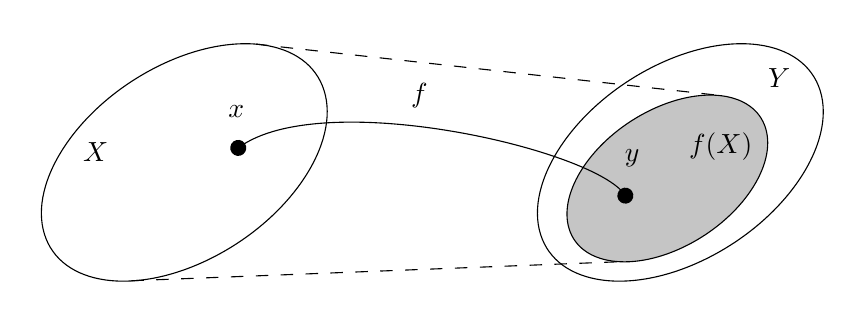
\begin{tikzpicture}[x=0.75pt,y=0.75pt,yscale=-1,xscale=1]
%uncomment if require: \path (0,300); %set diagram left start at 0, and has height of 300

%Shape: Ellipse [id:dp6106023081030485] 
\draw   (68.62,148.56) .. controls (60.81,123.39) and (84.66,87.51) .. (121.87,68.42) .. controls (159.09,49.34) and (195.58,54.27) .. (203.38,79.44) .. controls (211.19,104.61) and (187.34,140.49) .. (150.13,159.58) .. controls (112.91,178.66) and (76.42,173.73) .. (68.62,148.56) -- cycle ;
%Shape: Ellipse [id:dp5169799387829498] 
\draw   (307.62,148.56) .. controls (299.81,123.39) and (323.66,87.51) .. (360.87,68.42) .. controls (398.09,49.34) and (434.58,54.27) .. (442.38,79.44) .. controls (450.19,104.61) and (426.34,140.49) .. (389.13,159.58) .. controls (351.91,178.66) and (315.42,173.73) .. (307.62,148.56) -- cycle ;
%Straight Lines [id:da9434641726787872] 
\draw  [dash pattern={on 4.5pt off 4.5pt}]  (170.5,57) -- (394.93,81.83) ;
%Shape: Ellipse [id:dp39810559194245065] 
\draw  [fill={rgb, 255:red, 197; green, 197; blue, 197 }  ,fill opacity=1 ] (321.41,145.99) .. controls (315.93,128.31) and (332.68,103.11) .. (358.82,89.71) .. controls (384.95,76.31) and (410.58,79.77) .. (416.06,97.45) .. controls (421.54,115.13) and (404.79,140.32) .. (378.66,153.73) .. controls (352.52,167.13) and (326.89,163.67) .. (321.41,145.99) -- cycle ;
%Straight Lines [id:da574818986100407] 
\draw  [dash pattern={on 4.5pt off 4.5pt}]  (110.5,171) -- (345.93,161.83) ;
%Curve Lines [id:da8481099435063677] 
\draw    (162,107) .. controls (202,77) and (335,108) .. (348.5,130) ;
\draw [shift={(348.5,130)}, rotate = 58.47] [color={rgb, 255:red, 0; green, 0; blue, 0 }  ][fill={rgb, 255:red, 0; green, 0; blue, 0 }  ][line width=0.75]      (0, 0) circle [x radius= 3.35, y radius= 3.35]   ;
\draw [shift={(162,107)}, rotate = 323.13] [color={rgb, 255:red, 0; green, 0; blue, 0 }  ][fill={rgb, 255:red, 0; green, 0; blue, 0 }  ][line width=0.75]      (0, 0) circle [x radius= 3.35, y radius= 3.35]   ;

% Text Node
\draw (86,103.4) node [anchor=north west][inner sep=0.75pt]    {$X$};
% Text Node
\draw (416,67.4) node [anchor=north west][inner sep=0.75pt]    {$Y$};
% Text Node
\draw (378,98.4) node [anchor=north west][inner sep=0.75pt]    {$f( X)$};
% Text Node
\draw (156,85.4) node [anchor=north west][inner sep=0.75pt]    {$x$};
% Text Node
\draw (347,106.4) node [anchor=north west][inner sep=0.75pt]    {$y$};
% Text Node
\draw (244,74.4) node [anchor=north west][inner sep=0.75pt]    {$f$};


\end{tikzpicture}

      \caption{映射}
\end{figure}

映射这一术语, 在不同的数学领域中有不同的名称, 例如映射、变换、函数、算子等等.
严格来讲, 这些概念是有区别的, 但是这些区别最多也只是定义域与到达域取什么样的集合而已,
因此在本书中我们不强调这些概念的区别, 它们本质上都是映射.

在函数的定义中强调了对于给定的 $x \in X$, 按照函数 $f$ 与之相对应的 $y \in Y$
的唯一性, 换言之, 函数的概念允许多对一 (即对于不同的 $x_1,x_2 \in D$ 
可以有 $f(x_1) = f(x_2)$), 但不允许一对多 (即对于同一个 $x$ 同时有 $y_1 \ne y_2$
甚至更多的 $y \in Y$ 与之相对应).

显然 $f(X) \subset Y$, 即值域是到达域的一个子集. 特别地, 如果 $f(X) = Y$, 即值域与到达域
相等, 那么称 $f$ 是\textbf{满射} (surjection, onto). 
若 $\forall x_1,x_2 \in X \left( x_1 \ne x_2 \Longrightarrow
f(x_1) \ne f(x_2) \right)$, 即 $X$ 中不同元素 $x_1,x_2$ 在 $f$ 下的像不同
(即 $(f(x_1) = f(x_2)) \Longrightarrow (x_1 = x_2)$), 那么称 $f$ 是\textbf{单射} (injection, one-to-one).
如果 $f$ 既是单射又是满射, 那么称 $f$ 是\textbf{双射} (bijection, one-to-one correspondence).

\begin{figure}[H]
    \centering

\begin{minipage}{\textwidth}
\centering
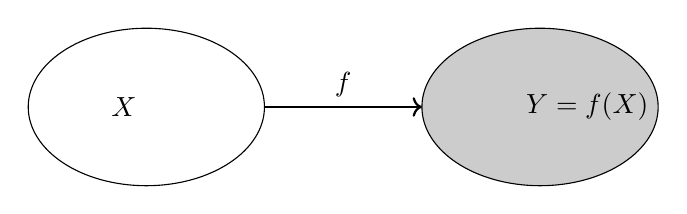
\begin{tikzpicture}
% 定义域 X
\draw (0,0) ellipse (1.5cm and 1cm) node[left] {$X$};
% 到达域 Y
\draw[fill=gray!40] (5,0) ellipse (1.5cm and 1cm);
\draw (6.5,0) node[left]{$Y=f(X)$};
% 映射箭头
\draw[->,thick] (1.5,0) -- node[above] {$f$} (3.5,0);
\end{tikzpicture}
\subcaption{满射}
\end{minipage}

\begin{minipage}{\textwidth}
\centering
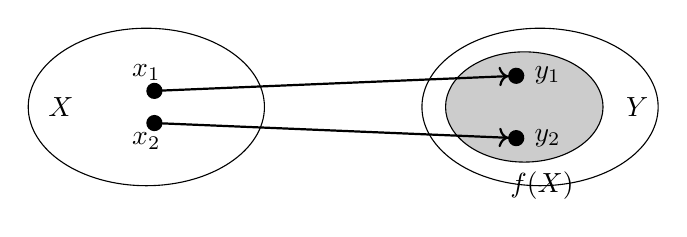
\begin{tikzpicture}
% 定义域 X
\draw (0,0) ellipse (1.5cm and 1cm);
\draw (-0.8,0) node[left]{$X$};
% 到达域 Y
\draw (5,0) ellipse (1.5cm and 1cm);
\draw (6.5,0) node[left]{$Y$};
% 值域 f(X)
\filldraw[fill=gray!40] (4.8,0) ellipse (1cm and 0.7cm);
\node at (4.5,-1) [right] {$f(X)$};
% 映射箭头
\draw[*->*,thick] (0,0.2) node[above]{$x_1$} -- (4.8,0.4) node[right]{$y_1$};
\draw[*->*,thick] (0,-0.2) node[below]{$x_2$} -- (4.8,-0.4) node[right]{$y_2$};
\end{tikzpicture}
\subcaption{单射}
\end{minipage}
      
\begin{minipage}{\textwidth}
\centering
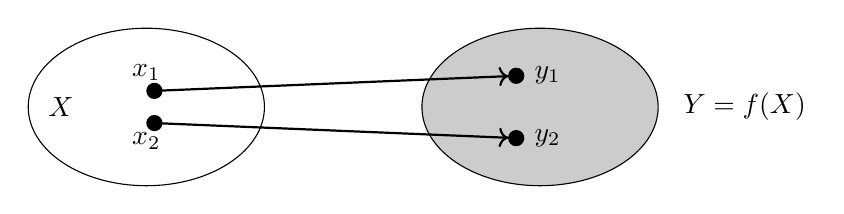
\begin{tikzpicture}
% 定义域 X
\draw (0,0) ellipse (1.5cm and 1cm);
\draw (-0.8,0) node[left]{$X$};
% 到达域 Y
\draw[fill=gray!40] (5,0) ellipse (1.5cm and 1cm);
\draw (8.5,0) node[left]{$Y=f(X)$};
% 映射箭头
\draw[*->*,thick] (0,0.2) node[above]{$x_1$} -- (4.8,0.4) node[right]{$y_1$};
\draw[*->*,thick] (0,-0.2) node[below]{$x_2$} -- (4.8,-0.4) node[right]{$y_2$};
\end{tikzpicture}
\subcaption{双射}
\end{minipage}
\caption{满射、单射、与双射}
\end{figure}

\subsection{函数的诸多例子}

接下来我们介绍一些函数, 它们有的是数学当中常用到的函数, 有的则是在自然科学和工程实践
中经常用到的函数.

\begin{example}
    函数 $y = |x| \xlongequal{\mathrm{def}} \begin{cases}
        -x, \quad \mathrm{if} \,\, x<0 \\
        x, \quad \mathrm{if} \,\, x\geqslant 0
    \end{cases}$
    称为\textbf{绝对值函数}, $\left| x \right|$ 表示 $x$ 的\textbf{绝对值}
    (absolute value). 它建立了一个函数关系 $\mathrm{abs}: \mathbb{R} \to \mathbb{R}^+$, 
    把任何一个实数 $x$ 变成它的绝对值, 即数轴上 $x$ 与原点之间的 “距离”\footnote{
        虽然我们现在还没有严格地定义距离的概念, 但我们在学习度量空间的理论的时候会知道,
        将绝对值称为 $\mathbb{R}$ 上的距离是合理且自然的.
    }. 它满足
    以下等式:
    \[ \boxed{\sqrt{x^2} = |x|}, \]
    这里一定要注意, 是一个易错点, 许多同学会误以为 $\sqrt{x^2} = x$, 但其实不是这样的,
    先平方后开根号的时候一定要考虑符号的影响 (因为平方本身会把这个数变成正数),
    例如, $\sqrt{(-2)^2} = \sqrt{4} = 2 = |-2|$.
    那么先开根号后平方呢? 由于我们要求根号 (这里指的是平方根号) 下的数是非负的,
    因此 $\left( \sqrt x \right)^2 = x \left( x \geqslant 0 \right)$.
\end{example}

插个题外话, 在数学中, 用两条竖线框住的一般都是表示数值, 例如, 如果 $x \in R$, 
那么 $|x|$ 表示
$x$ 的绝对值, 如果 $\boldsymbol{A}$ 是一个方阵, 那么 $|\boldsymbol{A}|$ 表示
$\boldsymbol{A}$ 的行列式, 如果 $z$ 是一个复数, 那么 $|z|$ 表示 $z$ 的模, 如果
$A$ 是一个集合, 那么 $|A|$ 表示集合 $A$ 中元素的个数. 不难发现, 它们都是数值.

\begin{example}
    $y = \mathrm{sgn} \, x \xlongequal{\mathrm{def}} \begin{cases}
        1, \quad \mathrm{if} \,\, x>0 \\ 
        0, \quad \mathrm{if} \,\,  x=0 \\ 
        -1, \quad \mathrm{if} \,\, x<0
    \end{cases}$ 称为\textbf{符号函数} (sign function), 它实际上建立了一个函数关系
    $\mathrm{sgn}: \mathbb{R} \to \left\{ -1,0,1 \right\}$,
    把正数变成 $1$,
    负数变成 $-1$, $0$ 变成 $0$.
\end{example}

\begin{figure}[H]
    \centering
    \begin{minipage}{0.4\textwidth}
        \centering
        \begin{tikzpicture}
            \draw[->] (-2.5,0) -- (2.5,0) node[right] {$x$};
            \draw[->] (0,-2.5) -- (0,2.5) node[above] {$y$};
            \draw (0,0) node[below right] {$O$};
            
            \draw (-2,2) -- (0,0);
            \draw (0,0) -- (2,2);
            
            \foreach \x in {-2,-1,1,2}
              \draw (\x,-0.1) -- (\x,0.1) node[above] {$\x$};
              
            \foreach \y in {-2,-1,1,2}
              \draw (-0.1,\y) -- (0.1,\y) node[right] {$\y$};
              
            \node at (1,1.5) [above right] {$y=|x|$};
        \end{tikzpicture}
        \subcaption{绝对值函数}
    \end{minipage}
    \begin{minipage}{0.4\textwidth}
        \centering
        \begin{tikzpicture}
            \draw[->] (-2.5,0) -- (2.5,0) node[right] {$x$};
            \draw[->] (0,-2.5) -- (0,2.5) node[above] {$y$};
            \draw[*-] (0,0) node[below right] {$O$};
            
            \foreach \x in {-2,-1,1,2}
            \draw (\x,-0.1) -- (\x,0.1) node[above] {$\x$};
            
            \foreach \y in {-2,-1,1,2}
            \draw (-0.1,\y) -- (0.1,\y) node[right] {$\y$};

            \draw[-o] (-2,-1) -- (0,-1);
            \draw[o-] (0,1) -- (2,1);
              
            \node at (1,1) [above right] {$y=\mathrm{sgn}\,x$};
        \end{tikzpicture}
        \subcaption{符号函数}
    \end{minipage}
    \caption{绝对值函数与符号函数}
\end{figure}

利用绝对值函数和符号函数, 我们可以把一个实数 $x$ 分成符号部分和数值部分, 这就是说,
对于任意给定的实数 $x$, 我们有 $x = \pm |x|$, 即 $x = (\mathrm{sgn}\,x) |x|$.
这一命题的分析表述为 $\forall x \in \mathbb{R} \left(
    x = (\mathrm{sgn}\, x)|x|
\right)$.

利用符号函数, 我们还可以写出一些仅利用命题逻辑和谓词逻辑不太好表达的命题的分析表述,
例如 {\kaishu 函数 $g(x)$ 在区间 $[a,b]$ 上不变号} 可以表述为
\[ \forall x_1, x_2 \in D \left(
    \mathrm{sgn}(g(x_1)) = \mathrm{sgn}(g(x_2))
\right). \]
这是相当自然的, 因为符号函数实现了一个数的符号与数值部分的分离, 因此只要一个区间 $[a,b]$
上任意给定的 $g(x_1), g(x_2)$ 的符号相同, 那么函数 $g$ 当然在这个区间上不变号.

\begin{example}
    函数 $\left\lfloor x \right\rfloor$ 表示 {\kaishu 不超过 $x$ 的最大整数},
    即 $x$ 的整数部分, 称为向下取整函数或者地板函数; 类似地, 可以定义 
    $\left\lceil x \right\rceil$ 为不小于 $x$ 的最小整数, 称为向上取整函数或
    天花板函数; $\left\lceil x \right\rfloor$ 称为向 $0$ 取整函数, 即取与 $0$
    最接近的且绝对值不超过 $|x|$ 的整数. 
    它们建立了从 $\mathbb{R}$ 到 $\mathbb{Z}$ 的一种函数关系, 显然, 这个关系是一个
    满射, 但不是一个单射 (例如, 实数 $1.1$ 和 $1.2$ 向下取整都是 $1$).
    我们可以把它们的严格的定义罗列如下:
    \begin{align*}
        \left\lfloor x \right\rfloor & \xlongequal{\mathrm{def}} \max \left\{
            n \in \mathbb{Z} | n \leqslant x
        \right\}, \\ 
        \left\lceil x \right\rceil & \xlongequal{\mathrm{def}} \min \left\{
            n \in \mathbb{Z} | n \geqslant x
        \right\}, \\
        \left\lceil x \right\rfloor & \xlongequal{\mathrm{def}} \begin{cases}
            \left\lceil x \right\rceil, \quad &\mathrm{if} \,\, x<0, \\ 
            \left\lfloor x \right\rfloor, \quad &\mathrm{if} \,\, x\geqslant 0.
        \end{cases}
    \end{align*}
    由于向下取整函数更为常用, 因此 $\left\lfloor x \right\rfloor$ 也记作 $[x]$,
    它满足一个重要的不等式:
    \[ \boxed{[x] \leqslant x < [x] + 1}, \]
    这里一定要注意, 一个数 $x$ 向下取整后仍然可以等于它本身 (如果它本来就是一个整数的话),
    但一个数绝对不可能等于或大于其向下取整再加 $1$ (即上述不等式的右边是严格小于而不是
    小于等于), 这是因为在向下取整的过程中被去掉的小数部分是严格小于 $1$ 的, 这一点在
    $[x]$ 的图像上也可以直观的感受到.
\end{example}
\begin{figure}[H]
    \centering
    \begin{tikzpicture}
        \draw[->] (-3.2,0) -- (3.2,0) node[right] {$x$};
        \draw[->] (0,-3.2) -- (0,3.2) node[above] {$y$};
        \draw (0,0) node[below right] {$O$};
        
        \foreach \x in {-3,-2,-1}
          \draw (\x,-0.1) -- (\x,0.1) node[above] {$\x$};
        \foreach \x in {1,2,3}
          \draw (\x,0.1) -- (\x,-0.1) node[below] {$\x$};
          
        \foreach \y in {-3,-2,-1,1,2,3}
          \draw (-0.1,\y) -- (0.1,\y) node[right] {$\y$};
          
        \foreach \x in {-3,-2,-1,1,2}
            \draw[*-o] (\x,\x) -- ({\x+1},\x);

        \foreach \x in {-3,-2,-1,1,2}
            \draw[dashed] (\x,\x) -- (\x,0);
        
        \draw[*-,dashed] (3,3) -- (3,0);
        \draw[dashed] (-3,-3) -- (3,3);
    \end{tikzpicture}
    \caption{向下取整函数, 你可以对照直线 $y=x$ (图中为斜向上的虚线) 来研究不等式
    $[x] \leqslant x < [x]+1$. 不难理解为什么该不等式左边是大于等于, 而右边却是
    严格小于.}
\end{figure}

\begin{example}
    公式 $l=2\pi r$ 和 $A = \pi r^2$ 建立了圆的周长 $l$ 和面积 $A$ 关于半径 $r$
    的函数关系, 这就是说, 它们建立了函数关系 $l: \mathbb{R}^+ \to \mathbb{R}^+$
    和 $A: \mathbb{R}^+ \to \mathbb{R}^+$, 前者把圆的半径变成它的周长, 后者把圆
    的半径变成了它的面积.
\end{example}

\begin{example}
    设 $E,M$ 是两个集合, 且 $E \subset M$. 在集合 $M$ 上, 按照如下条件确定
    $x \in M$ 对应的一个数 $\chi_E (x)$:
    \[ \chi_E(x) = \begin{cases}
        0, \quad & \mathrm{if} \,\, x \in M \setminus E, \\
        1, \quad & \mathrm{if} \,\, x \in E,
    \end{cases} \]
    该条件定义了函数关系 $\chi_E: M \to \left\{ 0,1 \right\}$, 我们将其称为集合
    $E$ 的\textbf{特征函数}. 我们比较熟悉的, 在分析中比较常用的一个特征函数, 是有理数集
    $\mathbb{Q}$ 在实数集 $\mathbb{R}$ 中的特征函数, 即 \textbf{Dirichlet 函数},
    记作 $D(x)$, 它建立了对应关系 $\chi_\mathbb{Q}: 
    \mathbb{R} \to \left\{ 0,1 \right\}$, 它的具体定义是:
    \[ D(x) = \begin{cases}
        0, \quad & \mathrm{if} \,\, x \in \mathbb{R} \setminus \mathbb{Q}, \\
        1, \quad & \mathrm{if} \,\, x \in \mathbb{Q},
    \end{cases} \]
    我们在分析中将会经常用到 Dirichlet 函数来构造一些典型问题的反例.
\end{example}

\begin{example}
    在计算机中, 所有的数据都以 0/1 二进制序列的形式来表示和处理. ASCII 称为\textbf{美国标准信息
    交换码} (American Standard Code for Information Interchange), 是一套成熟的
    西文编码方案, 它利用 7 个二进制位编码了 $2^7 = 128$ 个字符, 每个字符的 ASCII 码
    所对应的十进制数称为该字符的码值, 例如, \lstinline|a| 的码值为 97, \lstinline|A| 的
    码值为 $97 - 32 = 65$. 通过查表可知, 被编码的字符集与二进制数 0x00 至 0x7F 之间
    建立了一个双射. 事实上, 根据一一对应关系对每个被编码对象赋予唯一的编码就是编码工作的核心
    任务.
\end{example}

\setcounter{prop}{0}
\begin{prop}
    设 $A,B$ 是有限集合, 如果存在 $A$ 到 $B$ 的双射 $f$, 则 $|A| = |B|$,
    即 $A,B$ 的元素个数是相等的.
    \begin{proof}
        由于 $A,B$ 是有限集合, 设 $A = \left\{ a_1, a_2, \cdots, a_n \right\}$,
        由于 $f$ 是单射, 因此 $f(a_1), f(a_2), \cdots, f(a_n)$ 两两不相等, 而值域为
        \[ f(A) = \left\{ f(a_1), f(a_2), \cdots, f(a_n) \right\}, \]
        于是 $|f(A)| = n = |A|$, 又 $f$ 是满射, 所以 $f(A) = B$, 所以有
        $|A| = |f(A)| = |B|$.
    \end{proof}
\end{prop}
\begin{prop}
    设 $A,B$ 是有限集合, 有映射 $f: A \to B$, 且 $|A| = |B|$. 那么
    \begin{enumerate}[label=\textup{\arabic*}${}^\circ$, itemsep=0pt]
        \item 若 $f$ 是满射, 则 $f$ 是单射.
        \item 若 $f$ 是单射, 则 $f$ 是满射.
    \end{enumerate}
    \begin{proof}
        我们先证明 $1^\circ$, 假设 $f: A \to B$ 是满射, 即 $f(A) = B$,
         那么 $|f(A)| = |B|
        =|A| = n$, 于是 $f(a_1), f(a_2), \cdots,f(a_n)$ 一定两两不同, 否则的话
        它们就凑不出 $n$ 个元素了, 因此 $f$ 是单射.
        \newline 接下来我们来证明 $2^\circ$, 假设 $f$ 是单射, 
        即 $f(a_1), f(a_2), \cdots, f(a_n)$ 两两不相等, 从而
        $|f(A)| = n = |A| = |B|$, 又 $f(A) \subset B$, 因此 $f(A) = B$, 即 $f$
        是满射.
    \end{proof}
\end{prop}




\subsection{逆映射}

\begin{definition}[逆映射]
    设 $A,B$ 是两个集合,
    $f: A \to B$ 是一个映射, 如果对于 $B$ 中任意给定的元素 $b$, 在 $A$ 中存在
    唯一的元素 $a$ 使得 $f(a) = b$, 即
    \[ \forall b \in B \exists! a \in A \left( f(a) = b \right), \]
    那么这一条件实际上给出了从 $B$ 到 $A$ 的一个映射
    $g$, 将其称为 $f$ 的\textbf{逆映射} (inverse), 记作 $f^{-1}$, 此时称 $f$
    是可逆的.
\end{definition}

对于逆映射的概念, 我们稍微做一些说明.
逆映射的概念强调的是映射 $f:A \to B$ 下像 $b$ 的原像 $a$ 的唯一性而不是存在性.
根据映射的定义可知, $\forall a \in A \exists! b \in B \left( b=f(a) \right)$,
因此对于任意给定的 $b \in B$, 满足 $f(a) = b$ 的元素 $a \in A$ 总是存在的, 但映射关系
允许多对一, 但不允许一对多, 所以当 $a$ 不唯一时, 仅仅依照 $f(a) = b$ 这一关系是不能够
构造出从 $B$ 到 $A$ 的一个映射, 使得这个映射刚好把 $B$ 中的元素 $b = f(a)$ 给映射
回去. 所以, 我们要求对于值域中的每一个像, 可逆映射的原像要具有唯一性.

\begin{thm}
    映射 $f:A \to B$ 可逆的充分必要条件是 $f$ 是双射.
    \begin{proof}
        (必要性). 假设 $f: A \to B$ 可逆, 那么
        \[ \forall a \in A \exists ! b \in B \left( f(a) = b \right), \]
        \[ \forall b \in B \exists ! a \in A \left( f(a) = b \right), \]
        显然 $f(A) = B$, 并且由于对应于 $b$ 的原像 $a$ 的唯一性, 显然
        $f(a_1) \ne f(a_2) \Longrightarrow a_1 \ne a_2$, 因此 $f$ 是双射.
        \newline (充分性). 假设 $f: A \to B$ 是双射, 则
        由于 $f$ 是满射, $\forall b \in B \exists a \in A \left( f(a) = b \right)$,
        并且由于 $f$ 是单射, $b_1 \ne b_2 \Longrightarrow a_1 \ne a_2$,
        这就是说, $\forall b \in B \exists ! a \in A \left( f(a) = b \right)$,
        则 $f$ 可逆.
    \end{proof}
\end{thm}



\subsection{函数的复合}

\begin{definition}[复合函数]
    设 $f:X \to Y$, $g: W \to Z$ 是两个函数, 如果 $f(X) \cap W \ne \varnothing$,
    那么 \[ \forall x \in f(X)\cap W \exists! z \in Z \left(
        z = g(y) = g(f(x))
    \right),\] 那么这一关系实际上定义了 $X$ 到 $Z$ 的一个函数, 我们将其称为 $f$ 与
    $g$ 的\textbf{复合函数}, 记作 $g \circ f$.
\end{definition}

\begin{figure}[H]
    \centering
    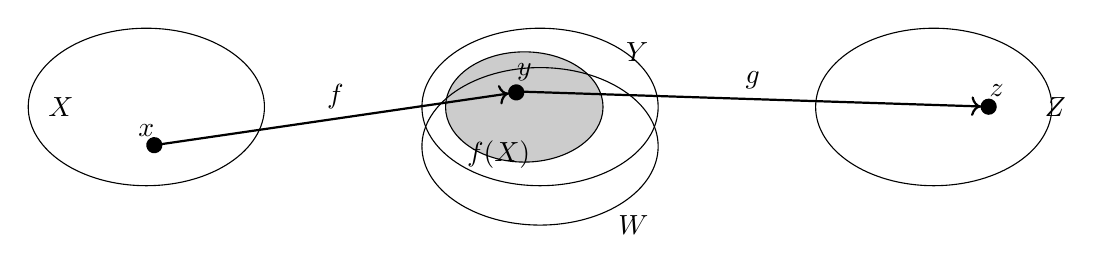
\begin{tikzpicture}[scale=1]
    % 定义域 X
    \draw (0,0) ellipse (1.5cm and 1cm);
    \draw (-0.8,0) node[left]{$X$};
    % 到达域 Y
    \draw (5,0) ellipse (1.5cm and 1cm);
    \draw (6.5,0.7) node[left]{$Y$};
    % 值域 f(X)
    \filldraw[fill=gray!40] (4.8,0) ellipse (1cm and 0.7cm);
    \node at (5,-0.6) [left] {$f(X)$};
    % 定义域 W
    \draw (5,-0.5) ellipse (1.5cm and 1cm);
    \draw (6.5,-1.5) node[left]{$W$};

    % 到达域 Z
    \draw (10,0) ellipse (1.5cm and 1cm);
    \draw (11.8,0) node[left]{$Z$};
    % 映射箭头
    \draw[*->*,thick] (0,-0.5) node[above]{$x$} 
    --node[midway, above]{$f$} (4.8,0.2) node[above]{$y$};
    \draw[->*, thick] (4.6,0.2)--node[midway, above]{$g$} (10.8,0) 
    node[above]{$z$};
    \end{tikzpicture}
    \caption{复合函数}
    \label{figure: 复合函数}
\end{figure}

函数的复合运算, 是定义在函数空间上的一种二元运算. 容易验证, 它具有结合律, 即
\[ (h \circ g) \circ f = h \circ (g \circ f), \]
并且利用数学归纳法很容易将其推广到有限个函数的复合,
因此我们在进行多个函数的复合时, 可以不必再写出括号, 也就是说, 当进行一连串函数的复合时,
我们可以直接写
\[ f_n \circ f_{n-1} \circ \cdots \circ f_2 \circ f_1, \]
而不需要在意加括号的情况.

两个函数能够复合的条件是内层函数 (即 $g(f(x))$ 里的 $f$, 即 $g \circ f$ 里的 $f$)
的值域与外层函数的交集不为空集, 这一交集同时也就成为了复合函数的定义域.

我们通常利用 \textbf{交换图} (commutative diagrams) 来描述函数之间的复合关系,
例如图 \ref{figure: 复合函数} 中展示的复合关系可以表示为
\begin{figure}[H]
    \centering
    \begin{tikzcd}
        X \arrow[r, "f"] \arrow[rd, "g \circ f"', bend right] & Y \arrow[d, "g"] \\
        & Z
    \end{tikzcd}
\end{figure}

\subsection{实值函数的基本性质}

接下来我们主要关注定义在实数域上的实值函数.
我们在这里学习到的各种性质, 称为函数的基本性质, 而在后面学习到的连续性、可微性、可积性,
则属于函数的微积分性质. 本节介绍函数的有界性、单调性、奇偶性和周期性.
% 在讨论性质的时候, 我们往往会把函数的性质按照其成立的范围分为
% 单点处的性质、局部性质、整体性质和全局性质和一致性质.
% \begin{itemize}[itemsep=0pt]
%     \item 单点处的性质是指这一性质仅在某一点上成立;
%     \item 局部性质是指这一性质在某点的一个邻域内成立;
%     \item 整体性质是指这一性质在一个区间上成立;
%     \item 全局性质是指这一性质在函数的整个定义域上成立;
%     \item 一致性质是指决定某整体性质的某个参数 (例如一致连续性的 $\delta$) 
%     在整个区间上保持不变, 而与该区间上具体的自变量 $x$ 的取值无关.
% \end{itemize}

\subsubsection{有界性}

有界性描述了函数在 $y$ 轴上分布的广度, 考虑一些 “有界的” 函数的例子, 例如 $\sin x$,
$\cos x$, 它们的图像都具有这样的特点, 即 {\kaishu 能够做出两条直线, 把函数在某一范围
内的图线 “框” 在这一范围内}, 由此我们抽象出有界函数的定义:

\begin{definition}[有界性]
    设函数 $f$ 在集合 $D$ 上有定义. 如果
    \begin{itemize}[itemsep=0pt]
        \item \textbf{上有界}: $\exists M \in R \forall x \in D \left(
            f(x) \leqslant M
        \right)$, 即{\kaishu 存在一个实数 $M$ 使得 $D$ 中任意的 $x$ 都成立 $f(x) \leqslant M$},
        则称 $f$ 在集合 $D$ 上 \textbf{上有界}, 
        $M$ 称为 $f$ 的\textbf{上界} (upper boundary).
        \item \textbf{下有界}: $\exists m \in R \forall x \in D \left(
            f(x) \geqslant m
        \right)$, 即{\kaishu 存在一个实数 $m$ 使得 $D$ 中任意的 $x$ 都成立 $f(x) \geqslant m$},
        则称 $f$ 在集合 $D$ 上 \textbf{下有界}, 
        $m$ 称为 $f$ 的\textbf{下界} (lower boundary).
        \item \textbf{有界}: $\exists M > 0 \forall x \in D \left(
            |f(x)| \leqslant M
        \right)$, 即{\kaishu 存在正数 $M$ 使得对于 $D$ 中任意给定的 $x$, 成立 $|f(x)| \leqslant M$},
        则称 $f$ 在集合 $D$ 上\textbf{有界}, 称 $f$ 是 $D$ 上的有界函数.
        \item \textbf{无界}: $\forall M>0 \exists x_0 \in D \left(
            |f(x)| \geqslant M
        \right)$, 则称 $f$ 在 $D$ 上 $\textbf{无界}$, 类似地可以给出 上无界 和
        下无界 的定义.
    \end{itemize}
    不难证明, {\kaishu 函数有界当且仅当它上有界且下有界}, 那么那个 $M$ 怎么构造呢?
    只需要取由上有界和下有界确定的 $M$ 和 $m$ 中, 绝对值更大的那一个的绝对值就好了,
    即 $\max \left\{ |M|,|m| \right\}.$
\end{definition}

\begin{remark}
    如果没有明确声明 $x$ 的范围, 而说 $f(x)$ 为有界函数, 那么就是指
    $f(x)$ 在其定义域上有界.
\end{remark}

\begin{example}
    指数函数 $y=\mathrm{e}^x$ 在整个定义域 $\mathbb{R}$ 内是一个下有界的函数,
    例如, $0$ 是它的一个下界, 因为 $\mathrm{e}^x > 0$ 在整个实数范围内总是
    成立的.
    \begin{figure}[H]
        \centering
        \begin{tikzpicture}
            \begin{axis}[
                xlabel=$x$,
                ylabel={$y$},
                axis lines=middle,
                xmin=-3.2, xmax=3.2,
                ymin=-1.2, ymax=10.2,
                domain=-3:3,
                samples=100,
                legend pos=north west,
            ]
            \addplot[thick] {exp(x)};
            \legend{$y = \mathrm{e}^x$}
            \end{axis}
        \end{tikzpicture}
        \caption{指数函数 $y=\mathrm{e^x}$}
    \end{figure}
\end{example}

\begin{example}
    Sigmoid 函数是在神经网络中非常常用的一个激活函数, 它的定义为
    \[ \mathrm{sigmoid}(x) \xlongequal{\mathrm{def}}
    \dfrac{1}{1+\exp(-x)}, \]
    它是一个定义在 $\mathbb{R}$ 上的有界函数. 这是因为 $\exp(-x) > 0$, 所以
    \[ 0 < \dfrac{1}{1+\exp(-x)} < 1, \]
    自然地, $0$ 成为它的一个下界, $1$ 成为它的一个上界.
    \begin{figure}[H]
        \centering
        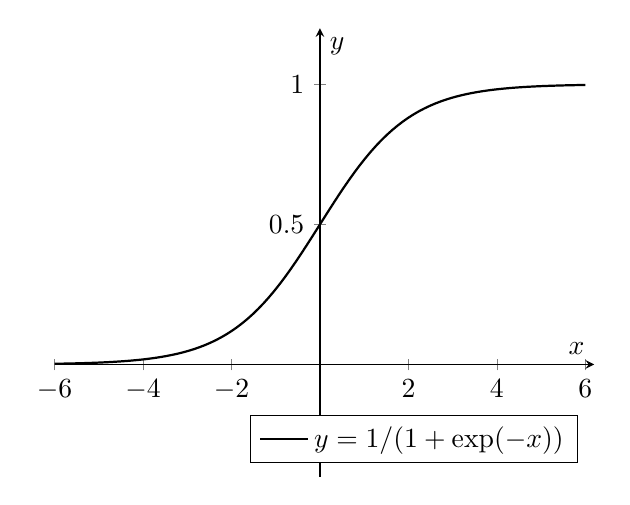
\begin{tikzpicture}
            \begin{axis}[
                xlabel=$x$,
                ylabel={$y$},
                axis lines=middle,
                xmin=-6, xmax=6.2,
                ymin=-0.4, ymax=1.2,
                domain=-6:6,
                samples=100,
                legend pos=south east,
            ]
            \addplot[thick] {1/(1 + exp(-x))};
            \legend{$y = 1/(1+\exp(-x))$}
            \end{axis}
        \end{tikzpicture}
        \caption{Sigmoid 函数}
    \end{figure}
\end{example}

\begin{example}
    函数 $f(x) = x \sin x$ 在其定义域 $\mathbb{R}$ 上是无界的.
    \begin{figure}[H]
        \centering
        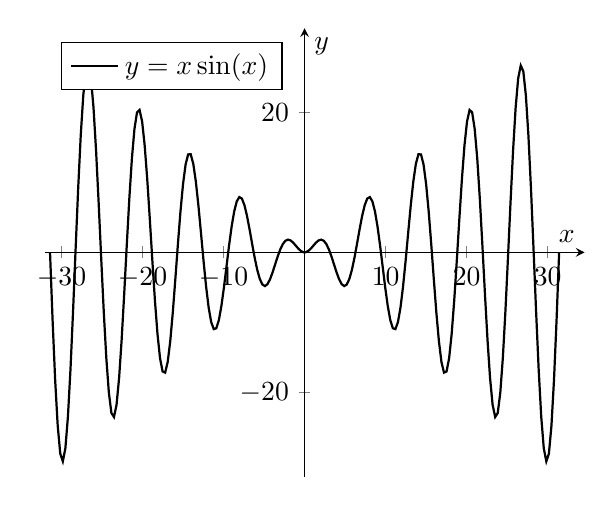
\begin{tikzpicture}
            \begin{axis}[
                xlabel=$x$,
                ylabel={$y$},
                axis lines=middle,
                xmin=-10.2*pi, xmax=11*pi,
                ymin=-32, ymax=32,
                domain=-10*pi:10*pi,
                samples=200,
                legend pos=north west,
            ]
            \addplot[thick] {x*sin(deg(x))}; % x*sin(x)
            \legend{$y = x\sin(x)$}
            \end{axis}
        \end{tikzpicture}
        \caption{$y = x \sin x$}
    \end{figure}
    \begin{proof}
        我们要证明函数 $x \sin x$ 无界, 按照定义, 其实就是要证明
        $\forall M>0 \exists x_0 \in \mathbb{R} \left(
            |x_0\sin x_0| \geqslant M
        \right)$. 但是由于正弦函数 $\sin x$ 的存在, 函数值会随着 $x$ 的增长
        不断在 $-x$ 和 $x$ 这两条直线之间振荡. 考虑 
        $\sin \left( \dfrac{\pi}{2} + 2k\pi \right) = 1$, 
        其中 $k \in \mathbb{Z}$, 显然我们可以取 $\mathbb{R}$ 的无穷子集
        $\left\{ x_k = \dfrac{\pi}{2} + 2k\pi \right\}$, 
        得到 $f$ 在 $\left\{ x_k \right\}$ 上的限制 $f|_{\left\{x_k\right\}} =
        x_k \sin(x_k) = x_k$.
        那么要使得不等式
        \[ \left| x_k \sin (x_k) \right| = \left| x_k \right| \geqslant M \]
        成立, 只需要取任意一个 $x_k > [M]+1$. 这时候显然有
        \[ x_k > [M]+1 > M, \]
        而这就是函数无界的定义. 整理一下, $\forall M > 0 \exists
        x_k = \dfrac{\pi}{2} + 2k\pi > [M]+1 \left(
            f(x_k) > M
        \right)$.
    \end{proof}
    \begin{remark}
        本例说明了研究函数的其中一个重要的手段: 在数轴 $\mathbb{R}$ 上按照一定的规则
        取定一个数列来把函数 $f(x)$ \textbf{离散化}. 所以如果你还是不懂上面的证明思路
        的话, 我还有一种说法, 这种说法可能不够严谨, 但是对于学过编程的同学来说肯定更容易理解:
        \newline for $x_k$ in $\mathrm{range}\left( \dfrac{\pi}{2}, +\infty, 2\pi \right)$:
        \newline \indent 我们研究 $f(x)$ 在这些散点处的性质, 
        \newline \indent 显然在这些点处 $f(x_k) = x_k \sin(x_k) = x_k \sin \left( \dfrac{\pi}{2} \right) = x_k$,
        \newline \indent 而 $x_k$ 可以任意大, 使得它大于给定的正数 $M$.
        \newline 总而言之, 以后我们经常会使用离散化的方法来研究定义域是连续区间的函数,
        这些散点的性质在一定程度上也能够反映在整个连续区间上的性质.
    \end{remark}
\end{example}

\subsubsection{单调性}

函数的单调性, 反映了随着自变量 $x$ 的增大与减小, 因变量 $y$ 的变化情况. 这就要求
我们需要在定义域 $X$ 和到达域 $Y$ 中都定义序关系, 才能基于序关系来定义函数的单调性,
不过本课程主要研究的是定义在实数集上的实值函数, 这一序关系是我们所熟识的, 我们会在
后文中详细的介绍实数集上的序关系.

\begin{definition}[函数的单调性]
    设 $f$ 是定义在 $D$ 上的实值函数, 集合 $I \in D$, 如果:
    \begin{itemize}[itemsep=0pt]
        \item $\forall x_1,x_2 \in I \left(
            x_1 < x_2 \Longrightarrow f(x_1) \leqslant f(x_2)
        \right)$, 则称 $f$ 在 $I$ 上
        \textbf{单调递增} (monotonic increase);
        \item $\forall x_1,x_2 \in I \left(
            x_1 < x_2 \Longrightarrow f(x_1) \geqslant f(x_2)
        \right)$, 则称 $f$ 在 $I$ 上
        \textbf{单调递减} (monotonic decrease);
    \end{itemize}
    将上述定义中的不等式更改为严格的不等式, 则有:
    \begin{itemize}[itemsep=0pt]
        \item $\forall x_1,x_2 \in I \left(
            x_1 < x_2 \Longrightarrow f(x_1) < f(x_2)
        \right)$, 则称 $f$ 在 $I$ 上
        \textbf{严格单调递增} (strictly monotonic increase);
        \item $\forall x_1,x_2 \in I \left(
            x_1 < x_2 \Longrightarrow f(x_1) > f(x_2)
        \right)$, 则称 $f$ 在 $I$ 上
        \textbf{严格单调递减} (strictly monotonic decrease).
    \end{itemize}
    单调递增的函数, 与单调递减的函数, 统称为\textbf{单调函数} (monotonic function),
    单调递增与单调递减, 统称为\textbf{单调性} (monotonicity).
\end{definition}
\begin{remark}
    判断函数的单调性, 一般是两个方法: 一是利用函数单调性的定义, 二是利用一阶导数的正负.
\end{remark}
\begin{example}
    前文中提到的符号函数 $\mathrm{sgn}(x)$, 向下取整函数 $y = [x]$、
    指数函数 $y = \mathrm{e}^x$、Sigmoid 函数 $\mathrm{sigmoid}(x)
    = \dfrac{1}{1+\exp(-x)}$ 都是其整个定义域上的单调函数. 除了符号函数和
    向下取整函数以外, 它们都是严格单调的.
\end{example}
\begin{example}
    绝对值函数 $y = |x|$ 在 $(-\infty,0]$ 上单调递减, $[0,+\infty)$ 上单调递增.
\end{example}
\begin{example}
    正弦函数 $y = \sin x$ 在区间 
    $\left[ -\dfrac{\pi}{2} + 2k\pi, \dfrac{\pi}{2} + 2k\pi \right]$ 
    上单调递增, 其中 $k \in \mathbb{Z}$, 在
    $\left[ \dfrac{\pi}{2} + 2k\pi, \dfrac{3\pi}{2} + 2k\pi \right]$
    上单调递减.
\end{example}

\subsubsection{奇偶性}

设函数 $f: D \to \mathbb{R}$ 的定义域 $D$ 关于点 $x = 0$ 对称, 定义域关于 $x=0$
对称是一个函数具有奇偶性的必要条件, 如果 $D$ 不关于 $x=0$ 对称, 那么函数 $f$ 没有
奇偶性可言, 一定是一个非奇非偶函数.

\begin{definition}[奇函数和偶函数]
    如果函数 $f$ 满足:
    \begin{itemize}[itemsep=0pt]
        \item $\forall x \in D \left(
            f(-x) = -f(x)
        \right)$, 则称 $f$ 是 \textbf{奇函数};
        \item $\forall x \in D \left(
            f(-x) = f(x)
        \right)$, 则称 $f$ 是 \textbf{偶函数}.
    \end{itemize}
    否则称 $f$ 为\textbf{非奇偶非偶函数}.
    简单地说, 对奇函数输入取反则输出也取反, 而对偶函数的输入取反却不会对输出有任何影响.
\end{definition}

根据奇偶函数的定义立即得到奇偶函数的几何性质: 奇函数的图像关于 $(0,0)$ 点中心对称,
也就是说, 对于 $(0,0)$ 点一侧的点 $(x,y)$, 在另一侧一定有点 $(-x,-y)$ 与之相互对应;
而偶函数的图像关于直线 $x=0$ 轴对称, 即对于 $x=0$ 一侧的点 $(x,y)$, 在另一侧一定有
点 $(-x,y)$ 与之对应.

\begin{example}
    根据三角恒等式, 有
    \[ \sin(-x) = \sin x, \quad 
    \cos(-x) = \cos x, \]
    这一性质也可以利用单位圆上的三角函数线来验证, 在这里我们就先不多讲了,
    我们会在《三角学回顾》一章中详细介绍这些内容.
    上面的两个等式说明正弦函数 $\sin x$ 是一个奇函数, 而余弦函数 $\cos x$ 是一个
    偶函数. 从图像上来看, 正弦函数的图像关于 $(0,0)$ 点成中心对称, 而余弦函数的图像
    则关于直线 $x=0$ 称轴对称.
    \begin{figure}[H]
        \centering
        \begin{minipage}{0.4\textwidth}
            \centering
            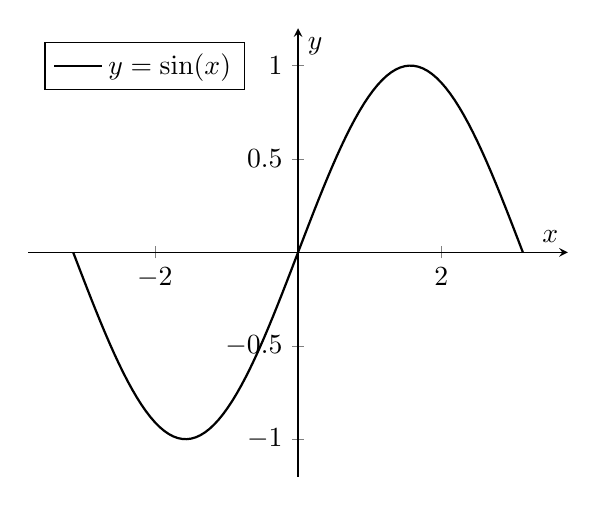
\begin{tikzpicture}
                \begin{axis}[
                    xlabel=$x$,
                    ylabel={$y$},
                    axis lines=middle,
                    xmin=-1.2*pi, xmax=1.2*pi,
                    ymin=-1.2, ymax=1.2,
                    domain=-1*pi:1*pi,
                    samples=100,
                    legend pos=north west,
                ]
                \addplot[thick] {sin(deg(x))}; % x*sin(x)
                \legend{$y = \sin(x)$}
                \end{axis}
            \end{tikzpicture}
            \subcaption{正弦函数}
        \end{minipage}
        \begin{minipage}{0.4\textwidth}
            \centering
            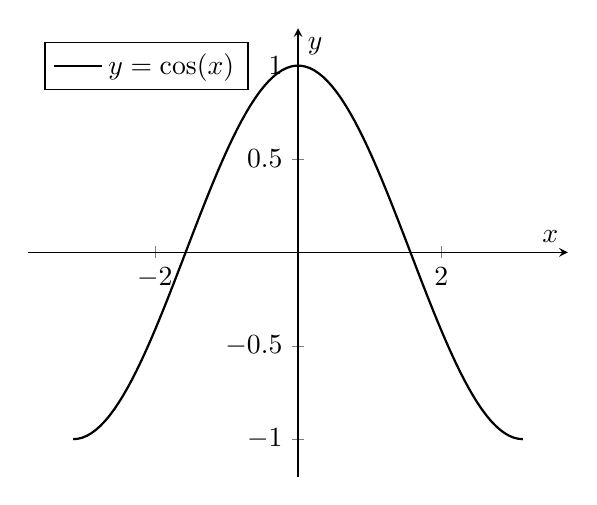
\begin{tikzpicture}
                \begin{axis}[
                    xlabel=$x$,
                    ylabel={$y$},
                    axis lines=middle,
                    xmin=-1.2*pi, xmax=1.2*pi,
                    ymin=-1.2, ymax=1.2,
                    domain=-1*pi:1*pi,
                    samples=100,
                    legend pos=north west,
                ]
                \addplot[thick] {cos(deg(x))}; % x*sin(x)
                \legend{$y = \cos(x)$}
                \end{axis}
            \end{tikzpicture}
            \subcaption{余弦函数}
        \end{minipage}
        \caption{两个三角函数在 $[-\pi,\pi]$ 上的图像}
    \end{figure}
\end{example}

根据奇偶函数的定义立即得到, 如果奇函数的定义域内包含点 $0$, 那么该点处的函数值
一定为 $0$, 我们将这一结论总结为如下性质:
\setcounter{property}{0}
\begin{property}
    设 $f: D \to \mathbb{R}$ 是一个奇函数, 如果 $0 \in D$, 那么
    $f(0) = 0$.
    \begin{proof}
        由于 $f$ 是奇函数, 所以 $f(-0)= f(0) = -f(0)$, 因此有 $f(0)=0$.
    \end{proof}
\end{property}

\subsubsection{周期性}

周期性描述了函数 $f$ 的输出 $y$ 随着自变量 $x$ 的变化的过程中出现的循环往复的现象,
或者说, 当自变量 $x$ 增加某一特定的数值时, 因变量 $y$ 的值就 “回到了起点”, 沿着
先前的变化规律再变化一次.

\begin{definition}[周期函数]
    设 $f: D \to \mathbb{R}$ 是一个函数, 如果
    $\exists T>0 \forall x \in D \left( (x+T) \in D \Longrightarrow
    f(x+T) = f(x) \right)$,
    这就是说, 如果{\kaishu 存在一个正数 $T$, 使得只要 $x+T$ 不超出
    定义域的范围, 就有 $f(x+T)=f(x)$}, 则称 $f$ 为 $D$ 上的\textbf{周期函数},
    满足上述条件的最小的正数 $\min \left\{ T>0 | \forall x \in D \left(
        (x+T) \in D \Longrightarrow f(x+T)=f(x)
    \right) \right\}$ 称为 $f$ 的\textbf{最小正周期} (least positive period,
    或 fundamental period).
\end{definition}
\begin{example}
    我们熟识的正弦函数、余弦函数都是周期函数, 它们的周期为 $2\pi$.
    % \begin{figure}[H]
    %     \centering
    %     \begin{minipage}{0.45\textwidth}
    %         \centering
    %         \begin{tikzpicture}
    %             \begin{axis}[
    %                 xlabel=$x$,
    %                 ylabel={$y$},
    %                 axis lines=middle,
    %                 xmin=-5.2*pi, xmax=5.2*pi,
    %                 ymin=-1.2, ymax=2,
    %                 domain=-5*pi:5*pi,
    %                 samples=200,
    %                 legend pos=north west,
    %                 % axis equal,
    %                 width=0.8\textwidth,
    %             ]
    %             \addplot[thick] {sin(deg(x))}; % x*sin(x)
    %             \legend{$y = \sin(x)$}
    %             \end{axis}
    %         \end{tikzpicture}
    %         \subcaption{正弦函数}
    %     \end{minipage}
    %     \begin{minipage}{0.45\textwidth}
    %         \centering
    %         \begin{tikzpicture}
    %             \begin{axis}[
    %                 xlabel=$x$,
    %                 ylabel={$y$},
    %                 axis lines=middle,
    %                 xmin=-5.2*pi, xmax=5.2*pi,
    %                 ymin=-1.2, ymax=2.0,
    %                 domain=-5*pi:5*pi,
    %                 samples=200,
    %                 legend pos=north west,
    %                 width=0.8\textwidth,
    %             ]
    %             \addplot[thick] {cos(deg(x))}; % x*sin(x)
    %             \legend{$y = \cos(x)$}
    %             \end{axis}
    %         \end{tikzpicture}
    %         \subcaption{余弦函数}
    %     \end{minipage}
    %     \caption{两个三角函数在 $[-5\pi,5\pi]$ 上的图像}
    % \end{figure}
\end{example}

\begin{example}
    $\tan x$, $\sin^2 x$ 和 $\left| \sin x \right|$ 
    都是周期函数, 它们的周期为 $\pi$.
\end{example}

\begin{example}
    Dirichlet 函数是周期函数, 且每一个有理数都是它的一个周期.
    \begin{proof}
        考虑 Dirichlet 函数 $D(x) = \begin{cases}
            0, \quad \mathrm{if} \,\, x \in \mathbb{R} \setminus \mathbb{Q}, \\ 
            1, \quad \mathrm{if} \,\, x \in \mathbb{Q},
        \end{cases}$, 我们将在后文中证明, {\kaishu 有理数集对加、减、乘、除四种运算封闭} 
        (于是我们将其称为有理数域), 而{\kaishu 无理数与有理数相加的结果为无理数}.
        利用这一结论, 我们知道对于任意给定的有理数 $T \in \mathbb{Q}$,
        如果 $x$ 为有理数, 那么 $x+T$ 仍为有理数, 因此有 $D(x) = D(x+T)$;
        同理, 如果 $x$ 为无理数, 那么 $x+T$ 仍为无理数, 因此 $D(x) = D(x+T)$.
        由此可见, 对于 Dirichlet 函数而言, 每一个有理数都是它的一个周期, 而且,
        Dirichlet 函数不存在最小正周期.
    \end{proof}
\end{example}

% \section{运算与运算律}

% 现代代数学研究的核心内容, 就是代数系统的结构及其保持运算性质的映射 (称为态射).

% 设 $S$ 是一个集合, 则 $S$ 上的 $n$ 个元素 $x_1, x_2, \cdots, x_n$ 构成的一个 $n$
% 元有序组 $(x_1, x_2, \cdots, x_n)$ 称为一个 $n$ \textbf{元组} (tuple).

% \begin{definition}
%     设 $A,B$ 是两个集合, 则所有形如 $(a,b)$ 的元组组成的集合
%     \[ A \times B := \left\{
%         (a,b) | a \in A \wedge b \in B
%     \right\} \]
%     称为 $A$ 与 $B$ 的一个 \textbf{Descartes 积}.
% \end{definition}

% 集合 $A$ 与它自身的 Descartes 积, 可以简记作 $A^2$.

% \begin{definition}[二元代数运算]
%     设 $S$ 是一个集合, 将映射 $f:S^2 \to S$ 称为 $S$ 的\textbf{二元代数运算}
%     (binary algebratic operation). 它把 $S$ 中的二元组 $x,y$ 变成 $S$ 中的另一个元素,
%     记作 $x \circ y$.
% \end{definition}

% 运算律指的是对于某个代数运算恒成立的等式. 在现代代数学中, 我们关注的运算律主要有:
% \begin{enumerate}[label={${\arabic*}^\circ$}, itemsep=0pt]
%     \item 交换律: $a \circ b = b \circ a$.
%     \item 结合律: $a \circ (b \circ c) = (a \circ b) \circ c$.
% \end{enumerate}

% \section{等价关系与集合的划分}
% \section{同态与同构}

\newpage
\thispagestyle{empty}

\part{数理逻辑、朴素集合论与布尔代数}


\chapter{布尔代数}

\section{布尔函数}

\subsection{基本布尔代数运算}

\textbf{布尔代数} (Boolean Algebra) 提供的是集合 $B := \left\{ 0,1 \right\}$ 上的运算和规则.
如果 $x \in B$, 则称它是一个\textbf{布尔变量} (Boolean variable),
它的值是且只可能是 $0$ 和 $1$ 中的一个.
最常用的三个布尔代数运算是补运算、布尔和以及布尔积. $x \in \left\{0,1\right\}$
的布尔补记作 $\bar x$, $x, y \in \left\{ 0, 1 \right\}$ 的布尔和与布尔积分别记作
$x+y$ 和 $x \cdot y$. 它们的定义由以下真值表给出:
\begin{table}[H]
    \centering
    \caption{基本布尔代数运算的真值表}
    \begin{tabular}{cc|ccc}
        \toprule
        $x$ & $y$ & $\bar x$ & $x+y$ & $x \cdot y$ \\ 
        \midrule
        0 & 0 & 1 & 0 & 0 \\ 
        0 & 1 & 1 & 1 & 0 \\ 
        1 & 0 & 0 & 1 & 0 \\ 
        1 & 1 & 0 & 1 & 1 \\ 
        \bottomrule
    \end{tabular}
\end{table}
容易看出, 两个布尔变量 $x,y$ 的布尔和取 $0$ 当且仅当 $x,y$ 都取 $0$, 因此布尔和又被称为
逻辑或运算, $x, y$ 的布尔积取 $1$ 当且仅当 $x, y$ 都取 $1$, 因此布尔积又被称为逻辑与运算,
而 $\bar x$ 与 $x$ 总是相反的, 因此也被称为逻辑取反运算.

在不引起混淆时, 也把 $x \cdot y$ 写成 $xy$ (就像代数积一样).

布尔运算的优先级从高到低分别是: 逻辑取反、布尔积、布尔和. 这与我们在代数中优先进行乘法、
在进行加法的习惯是一致的.

接下来我们给出布尔代数的抽象定义.

\begin{definition}[布尔代数]
    \label{def: boolean_algebra}
    布尔代数是一个集合 $B := \left\{0, 1\right\}$, 其上定义了两个二元运算 
    $(x,y) \mapsto x+y$ 和 $(x,y) \mapsto x \cdot y = xy$,
    以及一个一元运算 $x \mapsto \bar x$, 对于任意给定的 $x,y,z \in B$, 下列性质成立:
    \begin{enumerate}[label={$\left.\mathrm{B_\arabic*}\right)$}, itemsep=0pt]
        \item 同一律: $x+0 = x$, $x \cdot 1 = x$.
        \item 补律: $x + \bar x = 1$, $x\bar x = 0$.
        \item 结合律: $(x+y)+z = x+(y+z)$, $(xy)z = x(yz)$.
        \item 交换律: $x+y = y+x$, $xy = yx$.
        \item 分配律: $x+yz = (x+y)(x+z)$, $x(y+z) = xy+xz$.
    \end{enumerate}
\end{definition}

\subsection{布尔表达式和布尔函数}

\begin{definition}
    由布尔变量和布尔运算构成的表达式叫做布尔代数表达式, 它可以递归地定义为:
    \begin{enumerate}[label={${\arabic*}^\circ$}, itemsep=0pt]
        \item $0, 1, x_1, x_2, \cdots, x_n$ 是布尔表达式;
        \item 如果 $R_1, E_2$ 是布尔表达式, 则 $\bar E_1, E_1E_2, E_1 + E_2$ 是
        布尔表达式.
    \end{enumerate}
    换言之, 由 $n$ 个布尔变量 $x_1, x_2, \cdots, x_n \in B$ 经由有限次逻辑取反、布尔积与布尔和运算得到的
    表达式称为布尔代数表达式 (Boolean Algebratic expression).
\end{definition}



\begin{definition}
    函数 $f: B^n \to B$ 称为一个\textbf{布尔函数} (boolean function). 
\end{definition}

这就是说,
如果有一个法则 $f$ 使得
\[ \forall (x_1, x_2, \cdots, x_n) \in B^n
\exists ! y \in B \left( y=f(x_1, x_2, \cdots, x_n) \right), \]
那么它就规定了布尔 $n$ 元组 $(x_1, x_2, \cdots, x_n) \in B^n$ 到 
$B = \left\{0,1\right\}$
的一种对应关系. 同样, 布尔函数的值只可能是 $0$ 和 $1$ 当中的一个.
$B^n$ 是这个布尔函数的定义域, $B$ 是这个布尔函数的到达域. 每一个布尔变量 $x_i$
都是这个布尔函数 $f$ 的自变量, 而所有自变量取值的一种组合称为一个\textbf{指派},
与这个指派相对应的 $B$ 中的元素称为这个指派下的\textbf{值} (value).

一个布尔函数可以用布尔代数表达式来 “解析” 地表达, 也可以用真值表来穷举所有可能的指派及其
对应的取值.

\begin{definition}
    两个布尔函数 $f(x_1, x_2, \cdots, x_n)$ 与 
    $g(x_1, x_2, \cdots, x_n)$ 相等, 当且仅当它们对于每一个指派的值都相等.
    布尔函数 $f,g$ 的逻辑取反、布尔积与布尔和分别定义为:
    \begin{enumerate}[label={${\arabic*}^\circ$}, itemsep=0pt]
        \item $\bar f(x_1, x_2, \cdots, x_n) = \overline{
            f(x_1, x_2, \cdots, x_n)
        }$,
        \item $(f+g)(x_1, x_2, \cdots, x_n)
        = f(x_1, x_2, \cdots, x_n) + g(x_1, x_2, \cdots, x_n)$;
        \item $(fg)(x_1, x_2, \cdots, x_n)
         = f(x_1, x_2, \cdots, x_n) \cdot (x_1, x_2, \cdots, x_n)$.
    \end{enumerate}
\end{definition}

\subsection{布尔代数恒等式}

{\captionof{table}{布尔代数恒等式} % 表格标题
\label{布尔代数恒等式} % 交叉引用标签
\begin{longtable}{p{0.33\textwidth}|c||p{0.33\textwidth}|c}
    \toprule
    % 表头
    \textbf{恒等式} & \textbf{名称} & \textbf{恒等式} & \textbf{名称} \\

    \midrule
    \endhead
    \bottomrule
    \endfoot

    % 表格内容
        $\overline{\bar x} = x$ & 双重补律 & $x + yz = (x+y)(x+z)$
        
        $x(y+z) = xy+xz$& 分配律\\
        \hline
        $x+x = x$ 

        $x \cdot x = x$ & 幂等律 & $\overline{xy} = \bar x + \bar y$

        $\overline{x+y}=\bar x \bar y$ & De Morgan 律 \\ 
        \hline
        $x+0 = x$

        $x \cdot 1 = x$ & 同一律 & $x + xy=x$

        $x(x+y) = x$ & 吸收律 \\
        \hline 
        $x + 1 = 1$ 

        $x \cdot 0 = 0$ & 支配律 & $x + \bar x = 1$ & 单位元的性质 \\ 
        \hline 
        $x+y = y+x$

        $xy = yx$ & 交换律 & $x\bar x = 0$ 
        
        零元与单位元的性质统称为 “补律” & 零元的性质 \\ 
        \hline 
        $x+(y+z) = (x+y)+z$ 

        $x(yz) = (xy)z$ & 结合律 & & \\ 
\end{longtable}}

利用定义 \ref{def: boolean_algebra} 可以证明这些布尔恒等式. 实际上, 对比上表和布尔代数的
定义可以发现, 有些布尔恒等式直接出现在定义中, 而双重补律实际上只是零元的性质 $x \bar x = 0$
的推论, 因此需要我们证明的只有幂等律、支配律和 De Morgan 律.

\begin{example}
    证明布尔代数的幂等律 $x+x = x$, $x \cdot x = x$.
    \begin{proof}
        根据同一律, 我们知道 $x+0 = x$, 在这里我们基于补律, 把 $0$ 用 $x \bar x$ 代入,
        再利用布尔和关于布尔积的分配律得到
        \[ x = x + x \bar x = (x+x)(x + \bar x), \]
        我们注意到等号的右边 $x + \bar x$ 一项实际上为 $1$, 这就是说,
        \[ x = (x + x) \cdot 1, \]
        于是我们便证明了布尔和的幂等律. 同理, 利用同一律、补律和布尔积关于布尔和的分配律, 我们可以得到
        \[ x = x \cdot 1 = x (x + \bar x) = xx+x\bar x = xx + 0 = xx, \]
        这就是布尔积的幂等律.
    \end{proof}
\end{example}

\begin{example}
    证明布尔代数的支配律 $x+1=1$, $x\cdot 0 = 0$.
    \begin{proof}
        根据布尔代数的补律, 我们知道 $x + \bar x = 1$, 于是, 我们将 $x + 1$ 中的 $1$
        用 $x + \bar x$ 代入, 再利用布尔和的结合律, 得到
        \[ x+1 = x+\left( x+ \bar x \right) = \left( x+x \right) + \bar x, \]
        根据刚刚证明的布尔和的幂等律, 我们知道上式括号中的项 $x+x$ 其实就是 $x$, 因此,
        根据补律,
        \[ x+1 = (x+x) + \bar x = x+ \bar x = 1, \]
        这就是 $1$ 对布尔和的支配律. 同理, 根据补律、布尔积的幂等律和结合律, 我们有
        \[ x \cdot 0 = x \cdot \left( x \bar x \right) = \left( xx \right) \cdot \bar x 
        = x\bar x = 0, \]
        这就是 $0$ 对布尔积的支配律.
    \end{proof}
\end{example}

\begin{example}
    证明布尔代数的吸收律 $x+xy = x$, $x(x+y)=x$.
    \begin{proof}
        根据同一律, $x$ 实际上可以写成 $x \cdot 1$, 于是我们把 $x+xy$ 中的第一个 $x$
        用 $x \cdot 1$ 代入, 然后利用布尔积关于布尔和的分配律, 即可得到
        \[ x \cdot 1 + xy = x(1+y), \]
        根据我们刚刚证明的支配律, 等号的右边实际上就等于 $x \cdot 1$, 即 $x$.
        这就是布尔和的吸收律,
        同理, 根据布尔积关于布尔和的分配律和布尔积的幂等律,
        \[ x(x+y) = xx+xy = x+xy, \]
        这就转化为了我们刚刚证明的布尔和的吸收律, 因此, 布尔积的吸收律也得到证明了.
    \end{proof}
\end{example}

\begin{example}
    证明布尔代数的 De Morgan 律 $\overline{xy} = \bar x + \bar y$, 
    $\overline{x+y} = \bar x \bar y$.
    \begin{proof}
        要证明一个布尔变量是另一个布尔变量的补, 只要证明它们的布尔积为 $0$, 而布尔和为 $1$,
        事实上, 根据布尔积关于布尔和的分配律、布尔积的交换律和零元的性质,
        \[ xy\left( \bar x + \bar y \right) = xy\bar x + xy \bar y 
        = x \bar x y + xy \bar y = 0 \cdot y + x \cdot 0 = 0+0 =0,\]
        同理, 根据布尔和关于布尔积的分配律、布尔和的结合律, 以及刚刚证明的支配律, 我们有
        \[ xy + \left( \bar x + \bar y \right) 
        = \left(
            x+\left( \bar x + \bar y \right)
        \right) + \left(
            y+\left( \bar x + \bar y \right)
        \right) = x + \bar x + \bar y + y + \bar x + \bar y 
        = 1 + 1 + \bar x + \bar y = 1. \]
        这就证明了 $\overline{xy} = \bar x + \bar y$.
        接下来我们证明 $\overline{x+y} = \bar x \bar y$, 事实上,
        \[ (x+y)(\bar x \bar y)
        = x\bar x \bar y + y\bar x \bar y 
        = x \bar x \bar y + y \bar y \bar x 
        = 0 \cdot \bar y + 0 \cdot \bar x = 0+0 = 0, \]
        \[ (x+y) + \bar x\bar y =
        \left((x+y)+\bar x\right)\left((x+y)+\bar y\right)
        = \left( x+\bar x + y \right)\left( x+y +\bar y \right)
        = (1+y)(x+1) = 1 \cdot 1 = 1. \]
        这就是 De Morgan 定律.
    \end{proof}
\end{example}

\subsection{布尔代数恒等式、集合恒等式与逻辑等价式之间的关系}

一个令人振奋的好消息是, 对于一个给定的集合 $\varOmega$, 如果将其视为布尔常量 $1$,
将空集视为布尔常量 $0$, $A,B$ 是 $\varOmega$ 的子集, 而集合的交集、并集、补集分别
视为布尔积、布尔和以及布尔补的话, 就构成一个布尔代数. 于是表 \ref{集合恒等式} 中所列的
集合恒等式就都得到证明了. 

同理, 对于命题逻辑而言, 如果把逻辑常量 $\mathbf{T}$ 视为
布尔常量 $1$, 逻辑常量 $\mathbf{F}$ 视为布尔常量 $0$, 而命题的合取、析取、否定分别视为
布尔积、布尔和以及布尔补的话, 就构成一个布尔代数, 于是表 中所列的逻辑等价式
就都得到证明了.

这就是说, 你只需要记住他们三个其中的一个就足够了, 因为你可以从它们三者当中的任何一个等式出发,
得到同一等式在另外两种体系中的表示形式.

{\captionof{table}{布尔代数、集合运算与逻辑运算之间的关系} % 表格标题
\label{布尔代数、集合运算与逻辑运算之间的关系} % 交叉引用标签
\begin{longtable}{ccc}
    \toprule
    % 表头
    \textbf{布尔代数} & \textbf{数理逻辑} & \textbf{集合论} \\
    \toprule
    \endhead
    \bottomrule
    \endfoot

    % 表格内容
    $0$ & $\mathbf{F}$ & $\varnothing$ \\ 
    $1$ & $\mathbf{T}$ & $\varOmega$ \\ 
    布尔变量 $x$ & 逻辑命题 $x$ & $\Omega$ 的子集 $X$ \\
    $xy$ & $x \wedge y$ & $X \cap Y$ \\ 
    $x+y$ & $x \vee y$ & $X \cup Y$ \\
    $\bar x$ & $\lnot x$ & 补集 $\bar X$ \\
\end{longtable}}

% \section{布尔函数的析取范式}
% \section{布尔函数析取范式的化简}

% \chapter{关系}

% \section{关系及其性质}
% \section{关系的表示}
% \subsection{计算问题与探索性问题}

% \begin{exercise}
%     给定表示定义在有穷集上的关系的矩阵, 确定这个关系是否是自反的 (即具有反身性的) 或反自反的.
%     \begin{sol}
%         我们知道, 一个关系是自反的, 那么表示它的矩阵的主对角线上应该全为 $1$, 一个关系是反自反
%         的, 那么表示它的矩阵的主对角线上应该全为 $0$. 我们采用 \lstinline|numpy| 软件包
%         提供的 \lstinline|array| 数组来作为输入矩阵的存储结构.
%     \end{sol}
%     \begin{code} \lstinline|is_reflexive.py|
%         \begin{lstlisting}[language=Python]
% import numpy as np


% def is_reflexive(relationship: np.ndarray) -> bool:
%     if relationship.shape[0] != relationship.shape[1]: return False
%     return np.all(np.diag(relationship) == 1)

    
% relationship = np.array([[1, 1, 0],
%                             [1, 1, 1],
%                             [0, 1, 1]])
% print(is_reflexive(relationship))
%         \end{lstlisting}
%     \end{code}
% \end{exercise}



\newpage
\thispagestyle{empty}

\chapter{图}

图是由顶点和连接顶点的边构成的离散结构, 我们能够想到很多问题都可以用图来建模.
本章我们介绍图论的基本概念和基本的图模型, 然后介绍一些图论算法, 并分析它们的复杂度.

\section{图和图模型}

\subsection{图的基本概念}

\begin{definition}
    图 $G = (V, E)$ 由顶点 (或节点) 的非空集 $V$ 和边集 $E$ 构成, 每条边有一个或两个顶点
    与它相连, 这样的顶点称为边的端点.
    图 $G$ 的顶点集 $V$ 可能是无限的, 顶点集为无限集或有
    无限条边的图成为\textbf{无限图}, 相对的, 顶点集和边集为有限集合的图成为\textbf{有限图}.
\end{definition}

本章我们只考虑有限图.

每条边都连接着两个不同的顶点且自身没有两条不同的边连接一对相同顶点, 即没有任何一条边仅连接
一个顶点自身, 在两个顶点之间至多只有一条边 (要么没有, 要么只有一条) 的图称为\textbf{简单图}.
因此在简单图中, 一条边可以唯一地对应到顶点 $u, v$ 的一个无序偶 $\left\{ u, v \right\}$.

有多条边连接同一对顶点 $u, v$ 的图称为\textbf{多重图}, 连接顶点对 $\left\{ u, v \right\}$ 的
边的条数称为 $\left\{ u, v \right\}$ 的\textbf{多重度}.

把一个顶点连接到它自身的边称为\textbf{环}, 包含环或存在多重边的图称为\textbf{伪图}.

\begin{definition}
    \textbf{有向图} $(V, E)$ 有一个非空顶点集 $V$ 和一个有向边集 $E$ 组成, 每条有向边与一个顶点
    的有序对相关联. 与有序顶点组 $(u, v)$ 相关联的有向边开始于 $u$, 结束于 $v$.
\end{definition}

类似的, 我们有有向简单图、 有向多重图的概念. 此外, 如果一个图既有有向边又有无向边, 则称为
混合图.

\subsection{一些简单的图模型}

\begin{example}
    Obsidian 是一款以双向链接作为主要功能的知识管理软件, 在 Obsidian 中你可以通过
    双向链接语法 \lstinline|[[link]]| 来关联两个 \lstinline|Markdown| 文档.
    在 Obsidian 提供的 Graph View (局部关系图) 中, 一个文档是一个节点,
    被双链关联的两个文档会被用一条
    直线连接在一起. 如图 \ref{Abstract Algebra 词条的 Obsidian 局部关系图} 所示是词条 Abstract Algebra (抽象代数) 在我的 Obsidian 中的局部关系图
    的一个部分 (我并没有画出所有的节点和链接, 那样太浪费时间了), 你可以直观地通过局部关系图
    来看出与抽象代数有关系的课题分别是 Algebratic System (代数运算)、Algebra (代数)、
    Set (集合)、Algebratic Operation (代数运算)、Ring (环)、Field (域)、Group (群).
    \begin{figure}[H]
        \centering
        % 图的内容


        \tikzset{every picture/.style={line width=0.75pt}} %set default line width to 0.75pt        

        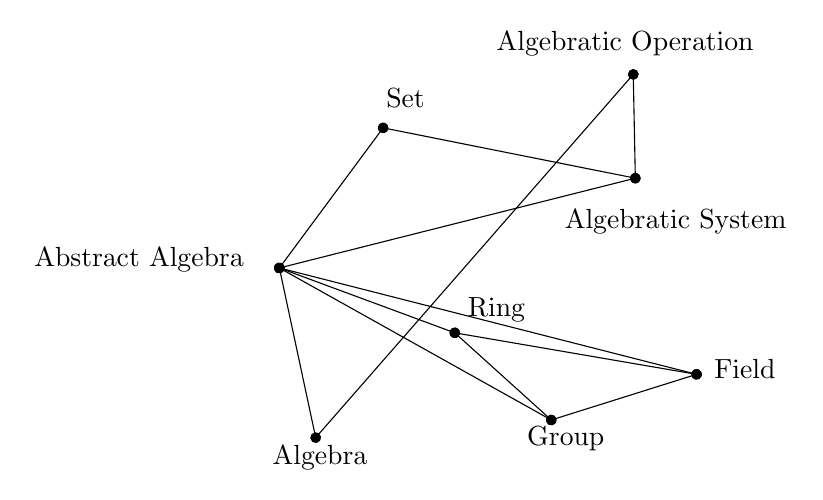
\begin{tikzpicture}[x=0.75pt,y=0.75pt,yscale=-1,xscale=1]
        %uncomment if require: \path (0,300); %set diagram left start at 0, and has height of 300
        
        %Straight Lines [id:da8846783151180141] 
        \draw    (207,133) -- (257,65.5) ;
        \draw [shift={(257,65.5)}, rotate = 306.53] [color={rgb, 255:red, 0; green, 0; blue, 0 }  ][fill={rgb, 255:red, 0; green, 0; blue, 0 }  ][line width=0.75]      (0, 0) circle [x radius= 2.01, y radius= 2.01]   ;
        \draw [shift={(207,133)}, rotate = 306.53] [color={rgb, 255:red, 0; green, 0; blue, 0 }  ][fill={rgb, 255:red, 0; green, 0; blue, 0 }  ][line width=0.75]      (0, 0) circle [x radius= 2.01, y radius= 2.01]   ;
        %Straight Lines [id:da2899931075424028] 
        \draw    (207,133) -- (224.5,214.75) ;
        \draw [shift={(224.5,214.75)}, rotate = 77.92] [color={rgb, 255:red, 0; green, 0; blue, 0 }  ][fill={rgb, 255:red, 0; green, 0; blue, 0 }  ][line width=0.75]      (0, 0) circle [x radius= 2.01, y radius= 2.01]   ;
        \draw [shift={(207,133)}, rotate = 77.92] [color={rgb, 255:red, 0; green, 0; blue, 0 }  ][fill={rgb, 255:red, 0; green, 0; blue, 0 }  ][line width=0.75]      (0, 0) circle [x radius= 2.01, y radius= 2.01]   ;
        %Straight Lines [id:da6762489335120624] 
        \draw    (207,133) -- (291.5,164.25) ;
        \draw [shift={(291.5,164.25)}, rotate = 20.3] [color={rgb, 255:red, 0; green, 0; blue, 0 }  ][fill={rgb, 255:red, 0; green, 0; blue, 0 }  ][line width=0.75]      (0, 0) circle [x radius= 2.01, y radius= 2.01]   ;
        \draw [shift={(207,133)}, rotate = 20.3] [color={rgb, 255:red, 0; green, 0; blue, 0 }  ][fill={rgb, 255:red, 0; green, 0; blue, 0 }  ][line width=0.75]      (0, 0) circle [x radius= 2.01, y radius= 2.01]   ;
        %Straight Lines [id:da970723977922583] 
        \draw    (291.5,164.25) -- (338,206.25) ;
        \draw [shift={(338,206.25)}, rotate = 42.09] [color={rgb, 255:red, 0; green, 0; blue, 0 }  ][fill={rgb, 255:red, 0; green, 0; blue, 0 }  ][line width=0.75]      (0, 0) circle [x radius= 2.01, y radius= 2.01]   ;
        \draw [shift={(291.5,164.25)}, rotate = 42.09] [color={rgb, 255:red, 0; green, 0; blue, 0 }  ][fill={rgb, 255:red, 0; green, 0; blue, 0 }  ][line width=0.75]      (0, 0) circle [x radius= 2.01, y radius= 2.01]   ;
        %Straight Lines [id:da0026328922586358328] 
        \draw    (291.5,164.25) -- (408,184.25) ;
        \draw [shift={(408,184.25)}, rotate = 9.74] [color={rgb, 255:red, 0; green, 0; blue, 0 }  ][fill={rgb, 255:red, 0; green, 0; blue, 0 }  ][line width=0.75]      (0, 0) circle [x radius= 2.01, y radius= 2.01]   ;
        \draw [shift={(291.5,164.25)}, rotate = 9.74] [color={rgb, 255:red, 0; green, 0; blue, 0 }  ][fill={rgb, 255:red, 0; green, 0; blue, 0 }  ][line width=0.75]      (0, 0) circle [x radius= 2.01, y radius= 2.01]   ;
        %Straight Lines [id:da6050275809052806] 
        \draw    (377.5,39.75) -- (378.5,89.75) ;
        \draw [shift={(378.5,89.75)}, rotate = 88.85] [color={rgb, 255:red, 0; green, 0; blue, 0 }  ][fill={rgb, 255:red, 0; green, 0; blue, 0 }  ][line width=0.75]      (0, 0) circle [x radius= 2.01, y radius= 2.01]   ;
        \draw [shift={(377.5,39.75)}, rotate = 88.85] [color={rgb, 255:red, 0; green, 0; blue, 0 }  ][fill={rgb, 255:red, 0; green, 0; blue, 0 }  ][line width=0.75]      (0, 0) circle [x radius= 2.01, y radius= 2.01]   ;
        %Straight Lines [id:da9428494633036296] 
        \draw    (257,65.5) -- (378.5,89.75) ;
        \draw [shift={(378.5,89.75)}, rotate = 11.29] [color={rgb, 255:red, 0; green, 0; blue, 0 }  ][fill={rgb, 255:red, 0; green, 0; blue, 0 }  ][line width=0.75]      (0, 0) circle [x radius= 2.01, y radius= 2.01]   ;
        \draw [shift={(257,65.5)}, rotate = 11.29] [color={rgb, 255:red, 0; green, 0; blue, 0 }  ][fill={rgb, 255:red, 0; green, 0; blue, 0 }  ][line width=0.75]      (0, 0) circle [x radius= 2.01, y radius= 2.01]   ;
        %Straight Lines [id:da11250770177398217] 
        \draw    (224.5,214.75) -- (377.5,39.75) ;
        \draw [shift={(377.5,39.75)}, rotate = 311.16] [color={rgb, 255:red, 0; green, 0; blue, 0 }  ][fill={rgb, 255:red, 0; green, 0; blue, 0 }  ][line width=0.75]      (0, 0) circle [x radius= 2.01, y radius= 2.01]   ;
        \draw [shift={(224.5,214.75)}, rotate = 311.16] [color={rgb, 255:red, 0; green, 0; blue, 0 }  ][fill={rgb, 255:red, 0; green, 0; blue, 0 }  ][line width=0.75]      (0, 0) circle [x radius= 2.01, y radius= 2.01]   ;
        %Straight Lines [id:da8024101790142418] 
        \draw    (207,133) -- (338,206.25) ;
        \draw [shift={(338,206.25)}, rotate = 29.21] [color={rgb, 255:red, 0; green, 0; blue, 0 }  ][fill={rgb, 255:red, 0; green, 0; blue, 0 }  ][line width=0.75]      (0, 0) circle [x radius= 2.01, y radius= 2.01]   ;
        \draw [shift={(207,133)}, rotate = 29.21] [color={rgb, 255:red, 0; green, 0; blue, 0 }  ][fill={rgb, 255:red, 0; green, 0; blue, 0 }  ][line width=0.75]      (0, 0) circle [x radius= 2.01, y radius= 2.01]   ;
        %Straight Lines [id:da8584208838314771] 
        \draw    (207,133) -- (408,184.25) ;
        \draw [shift={(408,184.25)}, rotate = 14.3] [color={rgb, 255:red, 0; green, 0; blue, 0 }  ][fill={rgb, 255:red, 0; green, 0; blue, 0 }  ][line width=0.75]      (0, 0) circle [x radius= 2.01, y radius= 2.01]   ;
        \draw [shift={(207,133)}, rotate = 14.3] [color={rgb, 255:red, 0; green, 0; blue, 0 }  ][fill={rgb, 255:red, 0; green, 0; blue, 0 }  ][line width=0.75]      (0, 0) circle [x radius= 2.01, y radius= 2.01]   ;
        %Straight Lines [id:da6346936046074653] 
        \draw    (338,206.25) -- (408,184.25) ;
        \draw [shift={(408,184.25)}, rotate = 342.55] [color={rgb, 255:red, 0; green, 0; blue, 0 }  ][fill={rgb, 255:red, 0; green, 0; blue, 0 }  ][line width=0.75]      (0, 0) circle [x radius= 2.01, y radius= 2.01]   ;
        \draw [shift={(338,206.25)}, rotate = 342.55] [color={rgb, 255:red, 0; green, 0; blue, 0 }  ][fill={rgb, 255:red, 0; green, 0; blue, 0 }  ][line width=0.75]      (0, 0) circle [x radius= 2.01, y radius= 2.01]   ;
        %Straight Lines [id:da3254430001759636] 
        \draw    (207,133) -- (378.5,89.75) ;
        \draw [shift={(378.5,89.75)}, rotate = 345.85] [color={rgb, 255:red, 0; green, 0; blue, 0 }  ][fill={rgb, 255:red, 0; green, 0; blue, 0 }  ][line width=0.75]      (0, 0) circle [x radius= 2.01, y radius= 2.01]   ;
        \draw [shift={(207,133)}, rotate = 345.85] [color={rgb, 255:red, 0; green, 0; blue, 0 }  ][fill={rgb, 255:red, 0; green, 0; blue, 0 }  ][line width=0.75]      (0, 0) circle [x radius= 2.01, y radius= 2.01]   ;
        
        % Text Node
        \draw (86,122) node [anchor=north west][inner sep=0.75pt]   [align=left] {\begin{minipage}[lt]{78.13pt}\setlength\topsep{0pt}
        \begin{center}
        Abstract Algebra
        \end{center}
        
        \end{minipage}};
        % Text Node
        \draw (254.5,45.5) node [anchor=north west][inner sep=0.75pt]   [align=left] {\begin{minipage}[lt]{18.03pt}\setlength\topsep{0pt}
        \begin{center}
        Set
        \end{center}
        
        \end{minipage}};
        % Text Node
        \draw (340,103.5) node [anchor=north west][inner sep=0.75pt]   [align=left] {\begin{minipage}[lt]{84.93pt}\setlength\topsep{0pt}
        \begin{center}
        Algebratic System
        \end{center}
        
        \end{minipage}};
        % Text Node
        \draw (294.5,146) node [anchor=north west][inner sep=0.75pt]   [align=left] {\begin{minipage}[lt]{23.7pt}\setlength\topsep{0pt}
        \begin{center}
        Ring
        \end{center}
        
        \end{minipage}};
        % Text Node
        \draw (323,208) node [anchor=north west][inner sep=0.75pt]   [align=left] {\begin{minipage}[lt]{31.08pt}\setlength\topsep{0pt}
        \begin{center}
        Group
        \end{center}
        
        \end{minipage}};
        % Text Node
        \draw (413.5,175.5) node [anchor=north west][inner sep=0.75pt]   [align=left] {\begin{minipage}[lt]{24.83pt}\setlength\topsep{0pt}
        \begin{center}
        Field
        \end{center}
        
        \end{minipage}};
        % Text Node
        \draw (200,217) node [anchor=north west][inner sep=0.75pt]   [align=left] {\begin{minipage}[lt]{37.88pt}\setlength\topsep{0pt}
        \begin{center}
        Algebra
        \end{center}
        
        \end{minipage}};
        % Text Node
        \draw (308.5,17.5) node [anchor=north west][inner sep=0.75pt]   [align=left] {\begin{minipage}[lt]{95.71pt}\setlength\topsep{0pt}
        \begin{center}
        Algebratic Operation
        \end{center}
        
        \end{minipage}};
        
        
        \end{tikzpicture}
        % \includegraphics*[width=\textwidth]{imagefile}
    
        \caption{Abstract Algebra 词条的 Obsidian 局部关系图}
        \label{Abstract Algebra 词条的 Obsidian 局部关系图}
    \end{figure}
\end{example}

\begin{example}
    微信小程序的搜索功能可以显示出曾经使用过某款小程序的好友数\footnote{
        也许是考虑到隐私的问题, 后续版本的微信中移除了这一功能.
    } (便于讨论起见, 我们约定本人
    不在计数范围内), 现在已知 Avory, Bob, Charles, Devon 和 Eric 五个人中有两个人使
    用过某款小程序, 他们在搜索界面中看到的使用过同一小程序的数量标注在图 \ref{有多少个好友使用过这款微信小程序?} 
    中对应用户的节点旁边, 他们之间的好友关系
    通过图中的一条直线段给出, 你能找出使用过这款小程序的是哪两个人吗?
    \begin{figure}[H]
        \centering
        % 图的内容
            

        \tikzset{every picture/.style={line width=0.75pt}} %set default line width to 0.75pt        

        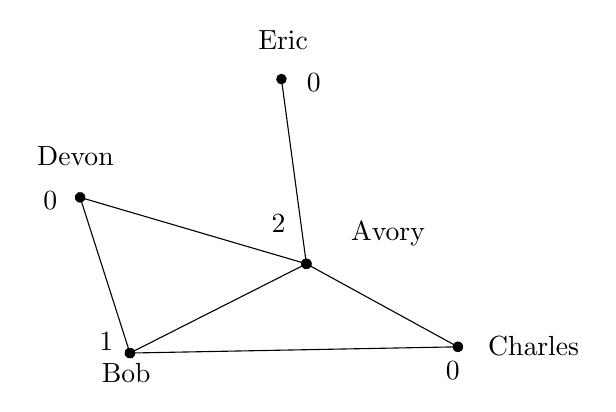
\begin{tikzpicture}[x=0.75pt,y=0.75pt,yscale=-1,xscale=1]
        %uncomment if require: \path (0,300); %set diagram left start at 0, and has height of 300

        %Straight Lines [id:da7447792705968247] 
        \draw    (291,165.5) -- (206,208.5) ;
        \draw [shift={(206,208.5)}, rotate = 153.17] [color={rgb, 255:red, 0; green, 0; blue, 0 }  ][fill={rgb, 255:red, 0; green, 0; blue, 0 }  ][line width=0.75]      (0, 0) circle [x radius= 2.01, y radius= 2.01]   ;
        \draw [shift={(291,165.5)}, rotate = 153.17] [color={rgb, 255:red, 0; green, 0; blue, 0 }  ][fill={rgb, 255:red, 0; green, 0; blue, 0 }  ][line width=0.75]      (0, 0) circle [x radius= 2.01, y radius= 2.01]   ;
        %Straight Lines [id:da8128743275169206] 
        \draw    (182,133.5) -- (206,208.5) ;
        \draw [shift={(206,208.5)}, rotate = 72.26] [color={rgb, 255:red, 0; green, 0; blue, 0 }  ][fill={rgb, 255:red, 0; green, 0; blue, 0 }  ][line width=0.75]      (0, 0) circle [x radius= 2.01, y radius= 2.01]   ;
        \draw [shift={(182,133.5)}, rotate = 72.26] [color={rgb, 255:red, 0; green, 0; blue, 0 }  ][fill={rgb, 255:red, 0; green, 0; blue, 0 }  ][line width=0.75]      (0, 0) circle [x radius= 2.01, y radius= 2.01]   ;
        %Straight Lines [id:da7297954163243963] 
        \draw    (182,133.5) -- (291,165.5) ;
        \draw [shift={(291,165.5)}, rotate = 16.36] [color={rgb, 255:red, 0; green, 0; blue, 0 }  ][fill={rgb, 255:red, 0; green, 0; blue, 0 }  ][line width=0.75]      (0, 0) circle [x radius= 2.01, y radius= 2.01]   ;
        \draw [shift={(182,133.5)}, rotate = 16.36] [color={rgb, 255:red, 0; green, 0; blue, 0 }  ][fill={rgb, 255:red, 0; green, 0; blue, 0 }  ][line width=0.75]      (0, 0) circle [x radius= 2.01, y radius= 2.01]   ;
        %Straight Lines [id:da8630614951535309] 
        \draw    (291,165.5) -- (279,76.5) ;
        \draw [shift={(279,76.5)}, rotate = 262.32] [color={rgb, 255:red, 0; green, 0; blue, 0 }  ][fill={rgb, 255:red, 0; green, 0; blue, 0 }  ][line width=0.75]      (0, 0) circle [x radius= 2.01, y radius= 2.01]   ;
        \draw [shift={(291,165.5)}, rotate = 262.32] [color={rgb, 255:red, 0; green, 0; blue, 0 }  ][fill={rgb, 255:red, 0; green, 0; blue, 0 }  ][line width=0.75]      (0, 0) circle [x radius= 2.01, y radius= 2.01]   ;
        %Straight Lines [id:da814920041604013] 
        \draw    (291,165.5) -- (364,205.5) ;
        \draw [shift={(364,205.5)}, rotate = 28.72] [color={rgb, 255:red, 0; green, 0; blue, 0 }  ][fill={rgb, 255:red, 0; green, 0; blue, 0 }  ][line width=0.75]      (0, 0) circle [x radius= 2.01, y radius= 2.01]   ;
        \draw [shift={(291,165.5)}, rotate = 28.72] [color={rgb, 255:red, 0; green, 0; blue, 0 }  ][fill={rgb, 255:red, 0; green, 0; blue, 0 }  ][line width=0.75]      (0, 0) circle [x radius= 2.01, y radius= 2.01]   ;
        %Straight Lines [id:da9305076421164262] 
        \draw    (206,208.5) -- (364,205.5) ;
        \draw [shift={(364,205.5)}, rotate = 358.91] [color={rgb, 255:red, 0; green, 0; blue, 0 }  ][fill={rgb, 255:red, 0; green, 0; blue, 0 }  ][line width=0.75]      (0, 0) circle [x radius= 2.01, y radius= 2.01]   ;
        \draw [shift={(206,208.5)}, rotate = 358.91] [color={rgb, 255:red, 0; green, 0; blue, 0 }  ][fill={rgb, 255:red, 0; green, 0; blue, 0 }  ][line width=0.75]      (0, 0) circle [x radius= 2.01, y radius= 2.01]   ;

        % Text Node
        \draw (310,144) node [anchor=north west][inner sep=0.75pt]   [align=left] {\begin{minipage}[lt]{28.61pt}\setlength\topsep{0pt}
        \begin{center}
        Avory
        \end{center}

        \end{minipage}};
        % Text Node
        \draw (189,212) node [anchor=north west][inner sep=0.75pt]   [align=left] {\begin{minipage}[lt]{20.88pt}\setlength\topsep{0pt}
        \begin{center}
        Bob
        \end{center}

        \end{minipage}};
        % Text Node
        \draw (374,199) node [anchor=north west][inner sep=0.75pt]   [align=left] {\begin{minipage}[lt]{37.87pt}\setlength\topsep{0pt}
        \begin{center}
        Charles
        \end{center}

        \end{minipage}};
        % Text Node
        \draw (157,108) node [anchor=north west][inner sep=0.75pt]   [align=left] {\begin{minipage}[lt]{32.2pt}\setlength\topsep{0pt}
        \begin{center}
        Devon
        \end{center}

        \end{minipage}};
        % Text Node
        \draw (265,52) node [anchor=north west][inner sep=0.75pt]   [align=left] {\begin{minipage}[lt]{20.29pt}\setlength\topsep{0pt}
        \begin{center}
        Eric
        \end{center}

        \end{minipage}};
        % Text Node
        \draw (163,129.4) node [anchor=north west][inner sep=0.75pt]    {$0$};
        % Text Node
        \draw (290,72.4) node [anchor=north west][inner sep=0.75pt]    {$0$};
        % Text Node
        \draw (273,140.4) node [anchor=north west][inner sep=0.75pt]    {$2$};
        % Text Node
        \draw (190,197.4) node [anchor=north west][inner sep=0.75pt]    {$1$};
        % Text Node
        \draw (357,211.4) node [anchor=north west][inner sep=0.75pt]    {$0$};


        \end{tikzpicture}
        % \includegraphics*[width=\textwidth]{imagefile}
    
        \caption{有多少个好友使用过这款微信小程序?}
        \label{有多少个好友使用过这款微信小程序?}
    \end{figure}
\end{example}

\subsection{复习参考题}

\begin{exercise}
    本节中介绍了许多简单的图模型, 你能说出这些图中哪些是无向图、哪些是有向图、哪些是简单图、
    哪些是多重图、哪些是带有环的图吗?
\end{exercise}

\section{图的术语和几种特殊的图}

\subsection{无向图的顶点和边}

\begin{definition}
    设 $G$ 为一个无向图. 若顶点 $u$ 和 $v$ 是 $G$ 中一条边 $e$ 的顶点, 则称 $u$ 和 $v$
    在 $G$ 中\textbf{邻接}, $e$ \textbf{连接}或者\textbf{关联} $u$ 和 $v$.
\end{definition}

\begin{definition}
    与顶点 $v$ 相邻的顶点和集合记作 $N(v)$.
\end{definition}

\begin{definition}
    在无向图中, 与顶点 $v$ 相关联的边的数目称为顶点 $v$ 的\textbf{度} (degree),
    记作 $\deg(v)$. 顶点上的环对顶点的度有双倍贡献.
\end{definition}

\begin{definition}
    如果点 $v$ 满足 $\deg(v) = 0$, 则称点 $v$ 是\textbf{孤立的},
    如果点 $v$ 满足 $\deg(v) = 1$, 则称点 $v$ 是\textbf{悬挂的}.
\end{definition}

从上述定义可知, 孤立点不与任何顶点相邻, 悬挂点与且仅与一个顶点相邻.

\begin{thm}[握手定理]
    设 $G = (V, E)$ 是有 $m$ 条边的无向图, 则
    \[ 2m = \sum_{v \in V}\deg(v), \]
    即无向图中所有顶点的度之和是它边数的两倍 (注意即使出现多重边和环, 该式也同样成立).
    \begin{proof}
        每条边恰好关联两个顶点, 因此每条边为 $\sum_{v \in V}\deg{v}$ 贡献 2.
    \end{proof} 
\end{thm}

\begin{thm}
    无向图 $G = (V,E)$ 中, 度为奇数的顶点有偶数个.
    \begin{proof}
        设 $V_1$ 和 $V_2$ 分别是度为奇数和偶数的顶点集, 显然 $V_1 \cap V_2 = \varnothing$
        且 $V_1 \cup V_2 = V$, 这是因为顶点的度要么为奇数, 要么为偶数, 且不存在度同时为
        奇数和偶数的顶点. 假设 $|E| = m$, 那么根据握手定理
        \[ 2m = \sum_{v \in V}\deg(v)
        = \sum_{v \in V_1}\deg(v) + \sum_{v \in V_2}\deg(v), \]
        其中 $2m$ 为偶数, $\sum_{v \in V_2}\deg(v)$ 为偶数, 因此
        $|V_1|$ 必须为偶数, 这是因为要保证偶数 $\sum_{v \in V_2}\deg(v)$
        与一个整数 $\sum_{v \in V_1}\deg(v)$ 的和为偶数 $2m$, 那么这个整数
        必须是偶数. 同时, 根据定义, $\sum_{v \in V_1}\deg(v)$ 是若干个奇数的和,
        要保证若干个奇数的和是一个偶数, 必须保证只有偶数个奇数参与求和.
    \end{proof}
\end{thm}

\subsection{有向图的顶点和边}

\begin{definition}
    设 $(u,v)$ 是有向图 $G$ 的边, 则称 $u$ \textbf{邻接到} $v$, 或
    $v$ 从 $u$ 邻接. 顶点 $u$ 称为边 $(u, v)$ 的起点, $v$ 称为边 $(u,v)$ 的终点.
    特别地, 环 $(u, u)$ 的起点和终点是相同的.
\end{definition}

\begin{definition}
    设 $G=(V, E)$ 是有向图, 以 $v$ 作为终点的边的数量称为顶点 $v$ 的\textbf{入度},
    记作 $\deg^-(v)$. 以 $v$ 为起点的边的数量称为顶点 $v$ 的\textbf{出度},
    记作 $\deg^+(v)$. 特别地, 环 $(v,v)$ 对顶点 $v$ 的出度和入度的贡献都是 $1$.
\end{definition}

\begin{thm}
    \label{进出守恒}
    设 $G = (V,E)$ 是有向图, 则它满足
    \[ \sum_{v \in V} \deg^-(v)
    = \sum_{v \in V} \deg^+(v) = |E|. \]
    \begin{proof}
        每条边都有一个起点和一个终点, 因此一条边对所有顶点入度之和、出度之和的贡献都是 1.
    \end{proof}
\end{thm}

你可以简单粗暴地把定理 \ref{进出守恒} 理解为 {\kaishu 在有向图中, 进入的总次数和离开的总次数
是相等的}, 这是因为一条边必然要 “离开” 它的起点然后 “进入” 它的终点. 请你不要想太多,
我只是在正常的介绍图论的知识而已, 脑子里不要总是装着这么多的 h 色废料.

\subsection{二分图}

\begin{definition}
    如果存在顶点集 $V$ 的一个划分 $(V_1, V_2)$, 使得图 $G = (V, E)$ 的每条边都连接 $V_1$
    中的一个顶点和 $V_2$ 中的一个顶点, 即 $G$ 中没有变连接 $V_1$ 中的两个顶点或
    $V_2$ 中的两个顶点, 则称 $G$ 为一个\textbf{二分图}.
\end{definition}

\begin{thm}
    \label{简单图是二分图的充分必要条件}
    一个简单图是二分图, 当且仅当存在一种赋值方案 (或者指派), 使得它的每个顶点都被赋予 
    $1$ 或 $0$ 的其中一个, 且没有两个相邻的顶点被赋予相同的值.
    \begin{proof}
        假设 $G = (V,E)$ 是简单二分图, 那么 $V = V_1 \oplus V_2$, 且
        \[ \forall e=\left\{v_1, v_2\right\} \in E \left(
            v_1 \in V_1 \wedge v_2 \in V_2
        \right), \]
        请读者自行验证该量化命题与二分图的定义等价.
        给 $V_1$ 中的所有顶点赋值 $0$, $V_2$ 中的所有顶点赋值 $1$ (反过来也可以),
        那么必然不存在一条边关联了两个所赋值相同的顶点, 否则 $G$ 就不是二分图了.
    \end{proof}
\end{thm}

定理 \ref{简单图是二分图的充分必要条件} 也可以表述为 “涂色”, 即 {\kaishu 简单二分图
的每个顶点都可以被涂上两种颜色中的一种, 并且相邻的顶点被涂上不同的颜色}. 总而言之,
这些表述都是类似的. 它的意义在于, 给我们提供了一种判断简单图是否为二分图的有效方法.

\subsection{从旧图构造新图}

本小节我们介绍从图构造出新图的若干办法, 例如子图、增加或删除图中的边、边的收缩、删除图中的顶点
和求两个图 (可以归纳地推广到更多个图) 的并集.

\subsubsection{子图}

\begin{definition}
    设 $G = (V, E)$ 是图, $W \subset V$, $F \subset E$ 是顶点集和边集的子集,
    如果图 $H = (W, F) \ne G$, 那么称 $G$ 的子图 $H$ 是 $G$ 的\textbf{真子图}.
\end{definition}

\begin{definition}
    设 $G = (V, E)$ 是简单图, $W$ 是边集 $V$ 的子集, 规定
    \[ F := \left\{ \left\{v_1, v_2\right\} \in E |
    v_1 \in W \wedge v_2 \in W \right\}, \]
    即边集 $F$ 是两个端点都在 $W$ 中的边的集合. 则称 $H = (W, F)$ 是由顶点集的子集 $W$
    \textbf{导出的子图}.
\end{definition}

% \subsubsection{增删图中的边}
% \subsubsection{边的收缩}
% \subsubsection{删除图中的顶点}
% \subsubsection{图的并集}

\newpage
\section{图的表示和图的同构}

% \subsection{邻接表}
% \subsection{邻接矩阵}
% \subsection{关联矩阵}
% \subsection{图的同构}

\begin{definition}
    设 $G_1 = (V_1, E_1)$, $G_2 = (V_2, E_2)$ 是简单图, 若存在双射 $f: V_1 \to V_2$
    使得{\kaishu 对于 $V_1$ 中任意给定的节点 $a,b$, 它们相邻当且仅当它们在 $V_2$ 中的像
    $f(a), f(b)$ 相邻}, 即
    \[ \forall a,b \in V_1 \left( \left\{ a,b \right\} \in E_1 
    \iff \left\{ f(a), f(b) \right\} \in E_2 \right). \]
    则称 $G_1$ 与 $G_2$ 是\textbf{同构的}, 双射 $f$ 称为 $G_1$ 与 $G_2$ 
    的\textbf{同构映射}.
\end{definition}
\setcounter{property}{0}
\begin{property}
    两个简单图的同构关系是等价关系.
    \begin{proof}
        要验证一个关系是等价关系, 只需证明它满足反身性、对称性和传递性\footnote{
            还记得吗? 关系 $\sim$ 是等价关系就是说: $a \sim a$ (反身性)、
            $a \sim b \vdash b \sim a$ (对称性)、$a \sim b, b \sim c \vdash 
            a \sim c$ (传递性).
        }. 而要验证图 $G_1$ 和 $G_2$
        同构, 关键是构造它们之间的同构映射.
        \begin{enumerate}[label={$\left.\mathrm{\alph*}\right)$}, itemsep=0pt]
            \item 反身性的证明: 只需取 $f$ 为恒等变换, 则 $G_1$ 与 $G_1$ 同构.
            \item 对称性的证明: 假设 $G_1$ 与 $G_2$ 同构, 即存在双射 $f$ 为 $G_1$ 与
            $G_2$ 的同构映射, 由于双射的逆映射是必然存在的, 因此取 $f^{-1}$ 作为 $G_2$
            与 $G_1$ 的同构映射即有 $G_2$ 与 $G_1$ 同构.
            \item 传递性的证明: 假设 $G_1$ 与 $G_2$ 同构, $G_2$ 与 $G_3$ 同构, 同构映射
            分别为 $f_{12}$ 和 $f_{23}$, 则 $f_{23} \circ f_{12}$ 仍为双射, 它可以作为
            $G_1$ 与 $G_3$ 的同构映射, 于是 $G_1$ 与 $G_3$ 同构.
        \end{enumerate}
        综上所述, 同构关系具有反身性、对称性和传递性, 它是一个等价关系.
    \end{proof}
\end{property}

% \newpage
% \section{连通性}



% \newpage
% \section{Euler 通路与 Hamilton 通路}
% \section{最短通路问题}
% \section{平面图}
% \section{图着色}

% \newpage
% \thispagestyle{empty}

% \chapter{归纳与递归}

% \section{递归算法}

% 如果一个算法通过把问题归约到带有更小输入的相同问题的实例来解决原来的问题, 则这个算法是递归的.
% 本节我们介绍若干的递归算法, 然后给出它们在 C、Java 或者 Python 中的实现, 并简要分析在递归
% 求解过程中递归算法是如何工作的.

% \begin{example}
%     给出计算 $n$ 的阶乘 $n!$ 的递归算法.
%     \begin{sol}
%         我们知道, $n! = n \cdot (n-1)!$, 而规定 $0! = 1! = 1$,
%         因此我们可以给出求 $n!$ 的递归算法
%         (使用 Python 语言描述) 为
%         \begin{lstlisting}[language=Python]
% def factorial(n: int) -> int:
%     return n * factorial(n - 1) if n != 1 and n != 0 else 1
%         \end{lstlisting}
%         表 \ref{example: factorial_3} 以计算 $3!$ 为例解释了算法是如何运行的, 该过程中调用栈的变化如表 \ref{example: factorial_3_stack} 所示.
%         {\captionof{table}{求解 $3!$ 的递归算法} % 表格标题
%         \label{example: factorial_3} % 交叉引用标签
%         \begin{longtable}{cccp{16em}}
%             \toprule
%             % 表头
%             \textbf{调用者} & \textbf{被调用者} & \textbf{返回值} & \textbf{对调用栈和现场的操作} \\
%             \toprule
%             \endhead
%             \bottomrule
%             \endfoot
        
%             % 表格内容
%             上级调用者 & \lstinline|factorial(3)| & \lstinline|3 * factorial(2)| & 入栈, 保留现场, \lstinline|factorial(2)| 入栈 \\
%             \lstinline|factorial(3)| & \lstinline|factorial(2)| & \lstinline|2 * factorial(1)| & 保留现场, \lstinline|factorial(1)|  入栈\\ 
%             \lstinline|factorial(2)| & \lstinline|factorial(1)| & \lstinline|1| & 出栈, 向 \lstinline|factorial(2)| 传递结果并恢复其现场 \\
%             \lstinline|factorial(2)| & \lstinline|factorial(2)| & \lstinline|2| & 出栈, 向 \lstinline|factorial(3)| 传递结果并恢复其现场 \\ 
%             上级调用者 & \lstinline|factorial(3)| & \lstinline|6| & 出栈, 将最终结果传递给上级调用者 \\
%         \end{longtable}}
%         {\captionof{table}{递归求解 $3!$ 的过程中调用栈的变化} % 表格标题
%         \label{example: factorial_3_stack} % 交叉引用标签
%         \begin{longtable}{|c|c|c|c|c|}
%             % 表头
%             \textbf{第一步} & \textbf{第二步} & \textbf{第三步} & \textbf{第四步} & \textbf{第五步} \\ 
            
%             \endhead
%             \endfoot
        
%             % 表格内容
%             && \lstinline|factorial(1)| && \\ 
%             & \lstinline|factorial(2)| & \lstinline|factorial(2)| & \lstinline|factorial(2)| & \\ 
%             \lstinline|factorial(3)| & \lstinline|factorial(3)| & \lstinline|factorial(3)| & \lstinline|factorial(3)| & \lstinline|factorial(3)| \\
%             上级调用者 & 上级调用者 & 上级调用者 & 上级调用者 & 上级调用者 \\
%             \hline
%         \end{longtable}}
%     \end{sol}
% \end{example}

% \begin{example}
%     给出计算非零实数 $a$ 的非负整数幂 $a^n$ 的递归算法.
%     \begin{sol}
%         我们知道, $a^n = a \cdot a^{n-1}$, 于是我们可以给出如下所示的递归算法:
% \begin{lstlisting}[language=Python]
% def power(a: float, n: int) -> float:
%     if n == 0:
%         return 1
%     if n == 1:
%         return a
%     return a * power(a, n-1)
% \end{lstlisting}
%     \end{sol}
% \end{example}

% \begin{example}
%     给出求满足 $a<b$ 的两个非负整数 $a$ 和 $b$ 的最大公因子的递归算法.
%     \begin{sol}
%         由于 $\gcd(a,b) = \gcd(b \mod a, a)$, 当 $b>0$ 时 $\gcd(0, b) = b$,
%         于是利用 Euclid 算法, 我们有
% \begin{lstlisting}[language=Python]
% def gcd(a: int, b: int) -> int:
%     if a == 0:
%         return b
%     else:
%         return gcd(b % a, a)
% \end{lstlisting}
%     \end{sol}
% \end{example}

\chapter{逻辑、推理与证明}


\section{命题等价式}




\begin{example}
    证明当 $n$ 是 $1 \leqslant n \leqslant 4$ 的正整数时, 有 $n^2 + 1 \geqslant2^n$.
\begin{proof}
    $n \in \left\{ n \in \mathbb{N^+} | 1 \leqslant n \leqslant 4 \right\} = {1,2,3,4}$, 当
\begin{enumerate}
        \item $n=1$ 时, $1^2 + 1 = 2 \geqslant 2^1 = 2$;
        \item $n=2$ 时, $2^2 +1 = 5 \geqslant 2^2 =4$;
        \item $n=3$ 时, $3^2 + 1 = 10 \geqslant 2^3 = 8$;
        \item $n=4$ 时, $4^2 + 1  = 17 \geqslant 2^4 = 16$,
\end{enumerate}
    因此对于任意的正整数 $n$, 只要 $1 \leqslant n \leqslant 4$, 就成立 $n^2 + 1 \geqslant 2^n$.
\end{proof}
\end{example}

\section{范式}

如何将命题公式转化为逻辑等价的标准形式? 这种标准形式就称为范式.

\subsection{析取范式和合取范式}

\begin{definition}
    命题公式中的一些命题变元和一些命题变元的否定之积, 称为\textbf{基本积},
    命题公式中的一些命题变元和一些命题变元的否定之和, 称为\textbf{基本和}.
\end{definition}

\begin{example}
    假设有三个命题变元 $p,q,r$, 那么 $p \wedge q \wedge (\lnot r)$ 就是它们的一个基本积,
    $p \wedge \lnot q$ 也是一个基本积.
\end{example}

\begin{thm}
    一个基本积是永假式, 当且仅当它含有 $p, \lnot p$ 形式的两个因子.
    一个基本和是永真式, 当且仅当它含有 $p, \lnot p$ 形式的两个因子.
    \begin{proof}
        T.B.C.
    \end{proof}
\end{thm}

\begin{definition}
    一个由基本积之和组成的公式, 如果与给定的命题公式 $A$ 等价, 则称它是 $A$ 的\textbf{析取范式}.
    记为 \[ A \iff A_1 \vee A_2 \vee \cdots \vee A_n, \quad (n \geqslant 1), \]
    这里 $A_1, A_2, \cdots, A_n$ 是基本积.
    类似地, 一个由基本和之积组成的公式, 如果与给定的命题公式 $A$ 等价, 则称它是 $A$
    的\textbf{合取范式}. 记为 \[ A \iff A_1 \wedge A_2 \wedge \cdots \wedge A_n, \quad (n \geqslant 1), \]
    这里 $A_1, A_2, \cdots, A_n$ 是基本和.
\end{definition}

\begin{example}
    求 $p \wedge (p \longrightarrow q)$ 的析取范式.
    \begin{sol}
        我们知道 $(p \longrightarrow q) \iff (\lnot p \vee q)$, 所以
        这一个命题公式实际上等价于
        \[ p \wedge (\lnot p \vee q), \]
        现在我们利用积关于和的分配律,
        \[ (p\wedge \lnot p) \vee (p \wedge q), \]
        显然 $p \wedge \lnot p$ 和 $p \wedge q$ 都是基本积. 它们的和就是原命题
        的析取范式. 现在我们把整个推理过程用逻辑联结符号再写一遍:
        \[ \begin{aligned}
            p \wedge (p \longrightarrow q) & \iff 
            p \wedge (\lnot p \vee q) \\ 
            & \iff (p\wedge \lnot p) \vee (p \wedge q).
        \end{aligned} \]
    \end{sol}
\end{example}

\begin{remark}
    析取范式、最简析取范式都未必唯一.
\end{remark}

\begin{example}
    证明 $q \vee p \wedge \lnot q \vee \lnot p \wedge \lnot q$ 是永真式.
    \begin{proof}
        整理, $q \vee (p \wedge \lnot q) \vee (\lnot p \wedge \lnot q)$,
        利用分配律, 分离出 $\lnot q$, 得到
        \[ q \vee (p \vee \lnot p) \wedge \lnot q, \]
        利用分配律,
        \[ (q \vee (p \vee \lnot p)) \wedge (q \vee \lnot q). \]
    \end{proof}
\end{example}

\subsection{主析取范式和主合取范式}

\begin{definition}
    在 $n$ 个变元的基本积中, 如果每一个变元预期否定不同时存在, 而两者之一必出现
    且仅出现一次, 则这种基本积称为\textbf{极小项}.
\end{definition}

$n$ 个变元可以构造出 $2^n$ 个极小项. 事实上, 极小项就是我们在真值表当中写出来的左边的
那 $n$ 列构成的命题. 例如, 命题 $p,q,r$ 的极小项为
\begin{table}[H]
    \centering
    \caption{极小项示例}
    \begin{tabular}{ccccc}
        \hline 
        $p$ & $q$ & 记号 & $r$ & 极小项 \\ 
        \hline
        0 & 0 & 0 & $m_0$ & $\lnot p \wedge \lnot q \wedge \lnot r$ \\ 
        0 & 0 & 1 & $m_1$ & $\lnot p \wedge \lnot q \wedge  r$\\ 
        0 & 1 & 0 & $m_2$ & $\lnot p \wedge  q \wedge \lnot r$\\ 
        0 & 1 & 1 & $m_3$ & $\lnot p \wedge  q \wedge  r$\\ 
        1 & 0 & 0 & $m_4$ & $ p \wedge \lnot q \wedge \lnot r$\\ 
        1 & 0 & 1 & $m_5$ & $ p \wedge \lnot q \wedge  r$\\ 
        1 & 1 & 0 & $m_6$ & $ p \wedge  q \wedge \lnot r$\\ 
        1 & 1 & 1 & $m_7$ & $ p \wedge  q \wedge  r$\\
        \hline
    \end{tabular}
\end{table}

\begin{definition}
    一个由极小项之和组成的公式, 如果与给定的命题公式 $A$ 等价, 则称它是 $A$ 的\textbf{主析取范式}.
\end{definition}

% \begin{example}
%     求 $A \equiv xzp \wedge q \vee r$ 的主析取范式.
% \end{example}

\subsection{使用真值表的方法}

这里介绍的方法非常重要, 一定要加以掌握.

\begin{example}
    求 $(p \rightarrow \lnot q) \rightarrow r$ 的主析取范式和主合取范式.
    \begin{sol}
        首先列出真值表
        \begin{table}[H]
            \centering
            \caption{$(p \rightarrow \lnot q) \rightarrow r$ 的真值表与极小项、极大项}
            \begin{tabular}{ccc|ccc|cc}
                \hline
                $p$ & $q$ & $r$ & $\lnot q$ & $p \to \lnot q$ & $(p \rightarrow \lnot q) \rightarrow r$ & 极小项 & 极大项 \\ 
                \hline 
                0 & 0 & 0 & 1 & 1 & 0 & $m_0$ & $M_0$ \\
                0 & 0 & 1 & 1 & 1 & 1 & $m_1$ & $M_1$ \\
                0 & 1 & 0 & 0 & 1 & 0 & $m_2$ & $M_2$ \\
                0 & 1 & 1 & 0 & 1 & 1 & $m_3$ & $M_3$ \\
                1 & 0 & 0 & 1 & 1 & 0 & $m_4$ & $M_4$ \\
                1 & 0 & 1 & 1 & 1 & 1 & $m_5$ & $M_5$ \\
                1 & 1 & 0 & 0 & 0 & 1 & $m_6$ & $M_6$ \\
                1 & 1 & 1 & 0 & 0 & 1 & $m_7$ & $M_7$ \\
                \hline
            \end{tabular}
        \end{table}
        接下来, 真值表中取值为真的项所对应的极小项 $m_i$ 构成主析取范式:
        \[ m_1 \vee m_3 \vee m_5 \vee m_6 \vee m_7, \]
        真值表中取值为假的项所对应的极大项 $M_i$ 构成主合取范式:
        \[ M_0 \wedge M_2 \wedge M_4. \]
    \end{sol}
\end{example}

\section{谓词逻辑}

一般地, 对于涉及 $n$ 个变元 $x_1,x_2,\cdots, x_n$ 的断言
\[ P(x_1,x_2,\cdots,x_n), \]
如果对于每一组给定的 $[x_1,x_2,\cdots,x_n]$, 都能够唯一确定真值 $1$ 或者 $0$
使得该真值与这一组给定的变元与之对应, 则称 $P(x_1,x_2,\cdots,x_n)$ 为一个\textbf{命题}
(proposition),
给定的 $[x_1,x_2,\cdots,x_n]$ 称为一个\textbf{指派}.



\newpage
\subsection{涉及量词的逻辑等价式}

\begin{definition}
    两个谓词和量词的语句 $S,T$, 如果满足:
    \begin{enumerate}[label={${\arabic*}^\circ$}, itemsep=0pt]
        \item 无论用什么谓词代入这些语句,
        \item 无论为这些命题函数里的变量指定什么论域,
    \end{enumerate}
    它们都具有相同的真值. 则称它们是\textbf{逻辑等价} (logical equivalent) 的,
    记作 $S \equiv T$.
\end{definition}

{\captionof{table}{涉及量词的逻辑等价式}
\begin{longtable}{p{0.4\textwidth}p{0.4\textwidth}}
    \toprule 
    \textbf{逻辑等价式} & \textbf{备注} \\ 
    \midrule
    \endfirsthead
    \multicolumn{2}{r}{(续表)} \\
    \toprule 
    \textbf{逻辑等价式} & \textbf{备注} \\ 
    \midrule
    \endhead

    \bottomrule
    \endfoot

    $(\forall x P(x)) \vee A \equiv \forall x \left(
        P(x) \vee A
    \right)$ & \\
    $(\exists x P(x)) \vee A \equiv \exists x \left(
        P(x) \vee A
    \right)$ \\ 
    $(\forall x P(x)) \wedge A \equiv \forall x \left(
        P(x) \wedge A
    \right)$ & \\
    $(\exists x P(x)) \wedge A \equiv \exists x \left(
        P(x) \wedge A
    \right)$ \\ 
    $\forall x \left( A \to P(x) \right) \equiv A \to \forall x P(x)$ \\ 
    $\exists x \left( A \to P(x) \right) \equiv A \to \exists x P(x)$ \\ 
    $\forall x \left( P(x) \to A \right) \equiv \exists x P(x) \to A$ \\ 
    $\exists x \left( P(x) \to A \right) \equiv \forall x P(x) \to A$ \\ 
    $\forall x \left( P(x) \wedge Q(x) \right) \equiv
    \forall x P(x) \wedge \forall x Q(x)$ \\ 
    $\exists x \left( P(x) \vee Q(x) \right) \equiv
    \exists x P(x) \vee \exists x Q(x)$
\end{longtable}}

% \begin{example}
%     证明 $\forall x P(x) \vee \forall x Q(x)$ 和 $\forall x \left( P(x) \vee Q(x) \right)$
%     不是逻辑等价的.
%     \begin{proof}
%         考虑论域 $\mathbb{R} \setminus \left\{0\right\}$, 这是所有非零实数的集合.
%         显然, $\forall x \in \mathbb{R} \setminus \left\{0\right\} \left(
%             x > 0 \vee x < 0
%         \right)$ 是成立的, 但
%         \[ \forall x \in \mathbb{R} \setminus \left\{0\right\} \left(
%             x>0
%         \right) \vee \forall x \in \mathbb{R} \setminus \left\{0\right\} \left(
%             x<0
%         \right) \]
%         却是一个假命题, 因为我们可以找到实数 $-1$ 使得量化命题
%         $\forall x \in \mathbb{R} \setminus \left\{0\right\} \left(
%             x>0
%         \right)$ 不成立, 也可以找到实数 $1$ 使得量化命题
%         $\forall x \in \mathbb{R} \setminus \left\{0\right\} \left(
%             x<0
%         \right)$ 不成立.
%     \end{proof}
% \end{example}

% \begin{example}
%     证明 $\exists x P(x) \wedge \exists x Q(x)$ 和 $\exists x \left(
%         P(x) \wedge Q(x)
%     \right)$ 不是逻辑等价的.
%     \begin{proof}
%         考虑实数集 $\mathbb{R}$ 作为论域, $(0, 1)$ 和 $(1, 2)$ 是它的两个子集, 设
%         $P(x) := x \in (0,1)$, $Q(x) := (1, 2)$, 那么显然
%         \[ \exists x P(x) \wedge \exists x Q(x) \]
%         是真命题, 这是因为你总是能在这两个开区间内找到两个实数. 但 
%         \[ \exists x \left( P(x) \wedge Q(x) \right) \]
%         是假命题, 这是因为这两个开区间的交集为空集, 你不可能找到同时属于它们二者的实数.
%     \end{proof}
% \end{example}

\begin{example}
    证明下列关系式.
    \begin{enumerate}[label={$\left.\arabic*\right)$}, itemsep=0pt]
        \item $\forall x \forall y \left( P(x) \vee Q(y) \right) \iff 
        \forall x P(x) \vee \forall y Q(y)$.
        \item $\exists x \exists y \left( P(x) \wedge Q(y) \right) \Longrightarrow \exists x P(x)$.
        \item $\forall x \forall y \left( P(x) \wedge Q(y) \right) \iff
        \forall x P(x) \wedge \forall y Q(y)$.
        \item $\forall x \forall y (P(x) \to Q(y)) \iff 
        \exists x P(x) \to \forall y Q(y)$.
    \end{enumerate}
    \begin{proof}
        \begin{enumerate}[label={$\left.\arabic*\right)$}, itemsep=0pt]
            \item 我们知道, $\forall x P(x) \vee A \equiv
            \forall x \left( P(x) \vee A \right)$, 其中 $A$ 为一个与 $x$ 无关的命题公式,
            取 $A = \forall y Q(y)$,
            \[ \begin{aligned}
                \forall x \left( P(x) \vee \forall y Q(y) \right) \equiv
                \forall x P(x) \vee \forall y Q(y),
            \end{aligned} \]
            同理, 在 $P(x) \vee \forall y Q(y)$ 中应用同样的法则, 即 $B \vee \forall y Q(y)
            \equiv \forall y \left( B \vee Q(y) \right)$, 取 $B = P(x)$, 这就得到
            \[ P(x) \vee \forall y Q(y) \equiv \forall y \left(
                P(x) \vee Q(y)
            \right), \]
            对命题公式 $\forall x \left( P(x) \vee \forall y Q(y) \right)$
            使用我们刚刚得到的逻辑等价式,
            \[ \forall x \left( P(x) \vee \forall y Q(y) \right)
            \equiv\forall x \left(
                \forall y \left(
                P(x) \vee Q(y)
            \right)
            \right), \]
            这是一个嵌套量词的命题, 但是注意到 $\forall x$ 和 $\forall y$ 的实际有效的作用域
            其实是重叠的, 所以可以把 $\forall y$ 提到外面来, 这就是说,
            \[ \forall x P(x) \vee \forall y Q(y)
            \equiv \forall x \forall y \left(
                P(x) \vee Q(y)
            \right). \]
            \item 下面几例中的证明思路都是类似的, 我们稍微写的简略一些. 为了证明
            原命题公式成立, 我们先证明
            $\exists x \exists y \left( P(x) \wedge Q(y) \right) \equiv
            \exists x P(x) \wedge \exists y Q(y)$. 事实上, 我们知道
            $\exists x P(x) \wedge A \equiv \exists x \left(
                P(x) \wedge A
            \right)$, 其中 $A$ 与 $x$ 无关. 取 $A = \exists y Q(y)$, 则有
            \[ \exists x P(x) \wedge \exists y P(y)
            \equiv \exists x \left( P(x) \wedge \exists y Q(y) \right)
            \equiv \exists x \left(
                \exists y \left(
                    P(x) \wedge Q(y)
                \right)
            \right)
            \equiv \exists x \exists y \left(
                    P(x) \wedge Q(y)
            \right).\]
            接下来我们要做的就是说明 
            $\exists x P(x) \wedge \exists y Q(y)
            \vdash \exists y P(y)$. 事实上根据推理规则的化简律
            $a \wedge b \vdash a$, 这是显然成立的.
            \item 我们知道, $\forall x P(x) \wedge A \equiv \forall x (P(x) \wedge A)$,
            其中 $A$ 与 $x$ 无关, 取 $A = \forall y Q(y)$, 得到
            \[ \forall x P(x) \wedge \forall y Q(y) \equiv
            \forall x \left( P(x) \wedge \forall y Q(y) \right)
            \equiv \forall x \left(
                \forall y \left( P(x) \wedge Q(y) \right)
            \right) \equiv \forall x \forall y \left(
                P(x) \wedge Q(y)
            \right). \]
            \item 我们知道, $\exists x P(x) \to A \equiv \forall x \left(
                P(x) \to A
            \right)$, 其中 $A$ 与 $x$ 无关, 取 $A = \forall y Q(y)$, 于是
            \[ \exists x P(x) \to \forall y Q(y) \equiv \forall x \left(
                P(x) \to \forall y Q(y)
            \right), \]
            在这里我们可以利用逻辑等价式 $\forall x \left(
                A \to P(x)
            \right) \equiv A \to \forall x P(x)$ 来直接得到结果,
            也可以对 $P(x) \to \forall y Q(y)$ 取逆否命题来把它化成
            $\exists x P(x) \to A \equiv \forall x \left(
                P(x) \to A
            \right)$ 能够处理的形式. 在这里我们选择后者,
            得到
            \[ 
            \begin{aligned}
                \forall x \left(
                    P(x) \to \forall y Q(y)
                \right) &\equiv \forall x \left(
                    \exists y \lnot Q(y) \to \lnot P(x)
                \right) \equiv
                \forall x \left(
                    \forall y \left(
                        \lnot Q(y) \to \lnot P(x)
                    \right)
                \right) \\ &\equiv
                \forall x \left(
                    \forall y \left(
                        P(x) \to Q(y)
                    \right)
                \right) \equiv \forall x \forall y \left(
                    P(x) \to Q(y)
                \right).
            \end{aligned} \]
        \end{enumerate}
        现在这四个关系式都得到证明了.
    \end{proof}
\end{example}

\begin{example}
    命题 $\exists y \in \mathbb{Z} \forall x \in \mathbb{Z} \left(
        y \times x = 0
    \right) = \mathbf{T}.$
    \begin{proof}
        只需要取 $y=0 \in \mathbb{Z}$ 即可.
    \end{proof}
\end{example}

\begin{example}
    $\forall x \in \left\{1,2\right\} \exists y \in \left\{1,2\right\}\left(
        x+y = 3
    \right) = \mathbf{T}$.
    \begin{proof}
        我们可以穷举 $x$ 和 $y$ 的所有可能的取值来验证这一命题是否为永真式.
        \captionof{table}{$\forall x \in \left\{1,2\right\} \exists y \in \left\{1,2\right\}\left(
            x+y = 3
        \right)$ 的验证}
        {\begin{longtable}{cccc}
            \toprule 
            $x$ & $y$ & $x+y$ & \textbf{$x+y = 3$ 的真值} \\
            \midrule 
            \endhead 

            \bottomrule
            \endfoot 

            $1$ & $1$ & $2$ & $0$ \\
            $1$ & $2$ & $3$ & $1$ \\
            $2$ & $1$ & $3$ & $1$ \\
            $2$ & $2$ & $4$ & $0$ \\
        \end{longtable}}
        {\noindent 注意到对于 $x$ 的每一个取值, 都能够找到一个 $y$ 使得 $x+y = 3$.}
    \end{proof}
\end{example}

\begin{example}
    设 $P(x, y)$ 是二元谓词, 论域 $D = \left\{ a,b \right\}$,
    在论域 $D$ 中谓词 $P$ 的真值如下表所示:
    {\captionof{table}{$P(x,y)$ 在 $D$ 中的定义}
    \begin{longtable}{ccc}
        \toprule 
        $x$ & $y$ & $P(x,y)$ \\
        \midrule 
        \endhead 

        \bottomrule
        \endfoot 

        $a$ & $a$ & $\mathbf{T}$ \\
        $a$ & $b$ & $\mathbf{F}$ \\
        $b$ & $a$ & $\mathbf{T}$ \\
        $b$ & $b$ & $\mathbf{F}$ \\
    \end{longtable}}
    {\noindent 求公式 $\forall x P(x, x)$, $\forall x \exists y P(x,y)$,
    $\exists x \exists y P(x,y)$ 的真值.}
    \begin{sol}
        上表实际上已经穷举了上述三个谓词逻辑命题的所有可能性,
        根据上表的第一行和第四行可以看出, $\forall x P(x, x) = \mathbf{F}$.
        由第一、第三行可知 $\forall x \exists y P(x,y) = \mathbf{T}$,
        $\exists x \exists y P(x,y) = \mathbf{T}$.
    \end{sol}
\end{example}

\subsection{前束范式}

\begin{definition}
    一个谓词逻辑语句, 如果它的形式满足
    \[ Q_1 x_1 Q_2 x_2 \cdots Q_k x_k P(x_1, x_2, \cdots, x_k), \]
    其中 $Q_i (i=1,2,\cdots, k)$ 要么是全称量词 $\forall$ 要么是存在量词 $\exists$. 并且
    $P(x_1, x_2, \cdots, x_k)$ 是不含量词的谓词, 那么称该语句为\textbf{前束范式}
    (prenex normal form, PNF).
\end{definition}

可以证明, 每个由命题变量、谓词、逻辑常量 $\mathbf{T}$ 和 $\mathbf{F}$ 与逻辑联结词和量词
构成的语句都等价于一个前束范式. 这称为\textbf{前束范式的存在性定理}. 我们将在后面用结构归纳法
证明这个定理.

\begin{example}
    将公式 $\forall x \left(
        A(x) \to B(x,y)
    \right) \to \left(\forall y \lnot C(y) \vee \exists z D(y,z)\right)$
    化为前束范式.
    \begin{sol}
        为了书写的更加简洁, 我们用 $P+Q$ 代替 $P \vee Q$, 用 $PQ$ 代替 $P \wedge Q$,
        用 $\bar P$ 代替 $\lnot P$.
        于是原命题公式可以等价的写作
        \[ \overline{\forall x \left( \overline{A(x)} + B(x,y) \right)}
        + \forall y \overline{C(y)} + \exists z D(y,z) \]
        将 $\forall y \overline{C(y)}$ 中的 $y$ 替换为 $u$, 同时利用 De Morgan 定律,
        \[ \text{上式} \equiv \exists x \left(
            A(x)\overline{B(x,y)}
        \right) + \left(\forall u \overline{C(u)} + \exists z D(y,z)\right), \]
        我们知道, $\exists x P(x) + A \equiv \exists x \left(
            P(x) + A
        \right)$, 于是令 $P(x) = A(x)\overline{B(x,y)}$, $A = \forall u \overline{C(u)} + \exists z D(y,z)$,
        得到 \[
            \text{上式} \equiv \exists x \left(
                A(x)\overline{B(x,y)}+ \left(
                    \forall u \overline{C(u)} + \exists z D(y,z)
                \right)
            \right) \equiv \exists x \left(
                A(x)\overline{B(x,y)}+ \forall u \overline{C(u)} + \exists z D(y,z)
            \right), \]
        同理, $\forall x P(x) + A \equiv \forall x \left(
            P(x) + A
        \right)$, 在此处取 $P(u) = \overline{C(u)}$, $A = A(x)\overline{B(x,y)} + \exists z D(y,z)$,
        则 \[ \text{上式} \equiv \exists x \left(
        \forall u \left( A(x)\overline{B(x,y)} + \exists z D(y,z) + \overline{C(u)} \right)
        \right), \]
        现在令 $P(z) = D(y,z)$, $A = A(x)\overline{B(x,y)} + \overline{C(u)}$,
        再次利用 $\exists x P(x) + A \equiv \exists x \left(
            P(x) + A
        \right)$ 即可将原谓词逻辑公式转化为其前束范式,
        \[ \text{上式} \equiv \exists x \forall u \exists z \left(
            A(x)\overline{B(x,y)} +  D(y,z) + \overline{C(u)}
        \right). \]
    \end{sol}
\end{example}

\section{推理规则}

\subsection{量化命题的推理规则}

\begin{table}[H]
    \centering
    \caption{量化命题的推理规则}
    \begin{tabular}{p{0.45\textwidth}p{0.45\textwidth}}
        \toprule
        \textbf{推理规则} & \textbf{名称} \\
        \midrule
        $\forall x P(x) \vdash P(c)$. & 全称实例 (universal instantiation) \\
        $P(c)$ for an arbitrary $c$ $\vdash \forall x P(x)$. & 全称引入 (universal generalization) \\
        $\exists x P(x)$ $\vdash P(c)$ for some element $c$. & 存在实例 (existantial instantiation) \\
        $P(c)$ for some element $c$ $\vdash \exists x P(x)$. & 全称引入 (existantial generalization) \\
        \bottomrule
    \end{tabular}
\end{table}

\begin{example}
    证明下列各断言: 
    \begin{enumerate}[itemsep=0pt, label={$\left.\arabic*\right)$}]
        \item $\lnot(\exists x P(x) \wedge Q(a)) \vdash \exists x P(x) \to \lnot Q(a)$.
        \item $\forall x \left(P(x) \vee Q(x)\right), \forall x \lnot P(x)
        \vdash \forall x Q(x)$.
        \item  $\lnot \forall x \left( P(x) \vee Q(x) \right), \forall x P(x)
        \vdash \lnot \forall x Q(x)$.
    \end{enumerate}
    \begin{proof}
        \begin{enumerate}[itemsep=0pt, label={$\left.\arabic*\right)$}]
            \item 下列步骤可以用来从前提 $\lnot(\exists x P(x) \wedge Q(a))$
            建立推论 $\exists x P(x) \to \lnot Q(a)$.
            {\begin{longtable}{p{0.45\textwidth}p{0.45\textwidth}}
                \toprule
            \textbf{步骤} & \textbf{理由} \\
            \midrule
            \endfirsthead

            \multicolumn{2}{r}{(续)} \\
            \toprule
            \textbf{步骤} & \textbf{理由} \\
            \midrule
            \endhead 

                \bottomrule
                \endfoot 

                1. $\lnot (\exists x P(x) \wedge Q(a))$. & 前提引入. \\
                2. $\forall x \left( \lnot P(x) \right) \vee \lnot Q(a)$.
                & 量化命题的否定规则. \\ 
                3. $\lnot P(c) \vee \lnot Q(a)$. & 全称实例. \\
                4. $P(c) \to \lnot Q(a)$ for some element $c$. & 命题恒等式 $a \to b \equiv \lnot a \vee b$. \\ 
                5. $\exists x \left( P(x) \right) \to \lnot Q(a) $. 
                & 特称引入. \\
            \end{longtable}}

            \item $\forall x \left(P(x) \vee Q(x)\right), \forall x \lnot P(x)
            \vdash \forall x Q(x)$.
            {\begin{longtable}{p{0.45\textwidth}p{0.45\textwidth}}
                \toprule
            \textbf{步骤} & \textbf{理由} \\
            \midrule
            \endfirsthead

            \multicolumn{2}{r}{(续)} \\
            \toprule
            \textbf{步骤} & \textbf{理由} \\
            \midrule
            \endhead

                \bottomrule
                \endfoot 

                1. $\forall x \left( P(x) \vee Q(x) \right)$.
                    & 前提引入. \\ 
                    2. $P(c) \vee Q(c)$. & 全称实例. \\
                    3. $\forall x \lnot P(x)$. & 前提引入. \\ 
                    4. $\lnot P(c)$. & 全称实例. \\ 
                    5. $Q(c)$ for an arbitrary $c$. & 析取三段论 $a \vee b, \lnot a \vdash b$. \\ 
                    6. $\forall x Q(x)$. & 全称引入. \\
            \end{longtable}}
        
            \item $\lnot \forall x \left( P(x) \vee Q(x) \right), \forall x P(x)
            \vdash \lnot \forall x Q(x)$.
            {\begin{longtable}{p{0.45\textwidth}p{0.45\textwidth}}
                \toprule
            \textbf{步骤} & \textbf{理由} \\
            \midrule
            \endfirsthead

            \multicolumn{2}{r}{(续)} \\
            \toprule
            \textbf{步骤} & \textbf{理由} \\
            \midrule
            \endhead

                \bottomrule
                \endfoot 

                1. $\lnot \forall x \left( P(x) \vee Q(x) \right)$ & 前提引入 \\
                2. $\exists x \left( \lnot P(x) \wedge \lnot Q(x) \right)$.
                & 量化命题的否定规则. \\
                3. $\lnot P(c) \wedge \lnot Q(c)$ for some element $c$.
                & 存在实例.\\
                4. $\lnot Q(c)$ for some element $c$. & 化简律 $a \wedge b \vdash a$. \\ 
                5. $\exists x \lnot Q(c)$. & 存在引入 \\ 
                6. $\lnot \forall x Q(x)$. & 量化命题的否定规则. \\
            \end{longtable}}
        \end{enumerate}
    \end{proof}
\end{example}

\begin{example}
    试用假设推理方法证明下面的定理:
    \begin{enumerate}[label={$\left.\arabic*\right)$}, itemsep=0pt]
        \item $\forall x \left(P(x) \to Q(x)\right) \vdash \left(
            \exists x P(x) \to \exists x Q(x)
        \right)$.
        \item $\forall x \forall y P(x,y) \to \forall y \forall x P(x,y)$.
        \item $\forall x \left( C(x) \to W(x) \wedge R(x) \right) \wedge
        \exists x \left(
            C(x) \wedge Q(x)
        \right) \to \exists x \left(
            Q(x) \wedge R(x)
        \right)$.
        \item $\lnot \exists x \left(
            F(x) \wedge H(x)
        \right) \wedge \forall x \left(
            G(x) \to H(x)
        \right) \to \forall x \left(
            G(x) \to \lnot F(x)
        \right)$.
    \end{enumerate}
    \begin{proof}
        \begin{enumerate}[label={$\left.\arabic*\right)$}, itemsep=0pt]
            \item 要证 $\forall x \left(P(x) \to Q(x)\right) \to \left(
                \exists x P(x) \to \exists x Q(x)
            \right)$, 只要证
            $\forall x \left(P(x) \to Q(x)\right)$, $\exists x P(x)
            \vdash \exists x Q(x)$.
            
            {\begin{longtable}{p{0.45\textwidth}p{0.45\textwidth}}
            \toprule
            \textbf{步骤} & \textbf{理由} \\
            \midrule
            \endfirsthead

            \multicolumn{2}{r}{(续)} \\
            \toprule
            \textbf{步骤} & \textbf{理由} \\
            \midrule
            \endhead

            \bottomrule
            \endfoot
            
            1. $\forall x \left(P(x) \to Q(x)\right)$ & 前提引入. \\ 
            2. $P(c) \to Q(c)$. & 全称实例. \\ 
            3. $\exists x P(x)$. & 前提引入. \\
            4. $P(c)$ for some element $c$. & 存在实例. \\ 
            5. $Q(c)$ for some element $c$. & 假言推理 $a \to b, a \vdash b$. \\ 
            6. $\exists x Q(x)$. & 存在引入. \\
            \end{longtable}}
            \item 要证 $\forall x \forall y P(x,y) \to \forall y \forall x P(x,y)$,
            只要证 $\forall x \forall y P(x,y) \vdash \forall y \forall x P(x,y)$.

            {\begin{longtable}{p{0.45\textwidth}p{0.45\textwidth}}
                \toprule
                \textbf{步骤} & \textbf{理由} \\
                \midrule
                \endfirsthead
    
                \multicolumn{2}{r}{(续)} \\
                \toprule
                \textbf{步骤} & \textbf{理由} \\
                \midrule
                \endhead
            \bottomrule
            \endfoot
            
            1. $\forall x \forall y P(x,y)$. & 前提引入. \\ 
            2. $P(m,n)$ for arbitrary $m,n$. & 全称实例. \\ 
            3. $\forall x P(x,n)$. & 全称引入. \\ 
            4. $\forall y \forall x P(x,y)$. & 全称引入. \\
            \end{longtable}}

            \item 要证 $\forall x \left( C(x) \to W(x) \wedge R(x) \right) \wedge
            \exists x \left(
                C(x) \wedge Q(x)
            \right) \to \exists x \left(
                Q(x) \wedge R(x)
            \right)$, 
            \newline 只要证 $\forall x \left( C(x) \to W(x) \wedge R(x) \right),
            \exists x \left(
                C(x) \wedge Q(x)
            \right) \vdash \exists x \left(
                Q(x) \wedge R(x)
            \right)$.

            {\begin{longtable}{p{0.45\textwidth}p{0.45\textwidth}}
                \toprule
                \textbf{步骤} & \textbf{理由} \\
                \midrule
                \endfirsthead
    
                \multicolumn{2}{r}{(续)} \\
                \toprule
                \textbf{步骤} & \textbf{理由} \\
                \midrule
                \endhead
                
                \bottomrule
                \endfoot
            
            1. $\forall x \left(
                C(x) \to W(x) \wedge R(x)
            \right)$. & 前提引入. \\ 
            2. $C(x) \to W(c) \wedge R(c)$. & 全称实例. \\ 
            3. $\exists x \left(
                C(x) \wedge Q(x)
            \right)$. & 前提引入. \\
            4. $C(c) \wedge Q(c)$ for some element $c$. & 存在实例. \\ 
            5. $C(c)$ for some element $c$. & 化简律 $a \wedge b \vdash a$. \\ 
            6. $W(c) \wedge R(c)$ for some element $c$. & 根据步骤 2, 利用假言推理 $a, a\to b \vdash b$. \\ 
            7. $R(c)$ for some element $c$. & 化简律 $a \wedge b \vdash a$. \\ 
            8. $Q(c)$ for some element $c$. & 根据步骤 4 利用化简律  $a \wedge b \vdash a$. \\ 
            9. $Q(c) \wedge R(c)$ for some element $c$. & 合取律 $a, b \vdash a \wedge b$. \\ 
            10. $\exists x \left(
                Q(x) \wedge C(x)
            \right)$. & 存在引入. \\
            \end{longtable}
            \item 要证 $\lnot \exists x \left(
                F(x) \wedge H(x)
            \right) \wedge \forall x \left(
                G(x) \to H(x)
            \right) \to \forall x \left(
                G(x) \to \lnot F(x)
            \right)$,
            \newline 只要证明 $\lnot \exists x \left(
                F(x) \wedge H(x)
            \right), \forall x \left(
                G(x) \to H(x)
            \right) \vdash \forall x \left(
                G(x) \to \lnot F(x)
            \right)$.

            \begin{longtable}{p{0.45\textwidth}p{0.45\textwidth}}
            \toprule
            \textbf{步骤} & \textbf{理由} \\
            \midrule
            \endhead
            \bottomrule
            \endfoot
            
            1. $\lnot \exists x \left(
                F(x) \wedge H(x)
            \right)$. & 前提引入. \\ 
            2. $\forall x \left(
                \lnot F(x) \vee \lnot H(x)
            \right)$. & 量化命题的否定规则. \\ 
            3. $\lnot F(c) \vee \lnot H(c)$ for arbitrary $c$.
            & 全称实例. \\
            4. $F(c) \to \lnot H(c)$. & 命题恒等式 $a \to b \equiv \lnot a \vee b$. \\ 
            5. $\forall x \left(
                G(x) \to H(x)
            \right)$. & 前提引入. \\ 
            6. $G(c) \to H(c)$ for arbitrary $c$. & 全称实例. \\
            7. $H(c) \to \lnot F(c)$. & 步骤 4 的逆否命题. \\ 
            8. $G(c) \to \lnot F(c)$ for arbitrary $c$. & 假言三段论 $a \to b, b \to c \vdash a \to c$. \\ 
            9. $\forall x \left(
                G(x) \to \lnot F(x)
            \right)$. & 全称引入. \\
            \end{longtable}}
        \end{enumerate}
    \end{proof}
\end{example}

\newpage
\begin{example}
    请证明 {\kaishu 发表所谓 “只有纯数学才是真正的数学, 别的都是垃圾” 言论的人可能并不热爱理论数学,
    或者这个人并没有最基本的尊重与修养}.
    \begin{proof}
        我们可以利用推理规则来不严格地从前提建立结论, 以下内容纯属娱乐, 并不是为了引战. 
        假设 $a$ 是一个人.
        {\begin{longtable}{p{0.45\textwidth}p{0.45\textwidth}}
            \toprule
            \textbf{步骤} & \textbf{理由} \\
            \midrule
            \endhead
            
            \bottomrule
            \endfoot
        
            $a$ 发表 “只有纯数学才是真正的数学” 的言论. & 前提引入. \\
            $a$ 在贬低/诋毁其他的数学分支. & 这是前提的简单推论. \\ 
            “己所不欲, 勿施于人”. & 我们在这里将其作为不需要证明的结论给出, 
            这是因为在各个文化中都能找到类似的表述. \\
            任何人都不希望别人贬低/诋毁自己热爱的事物. & 我们将其作为不需要证明的结论给出, 
            这是因为从经验出发来看, 有许多故事告诉我们自己所热爱的事物被诋毁是不能容忍的. \\ 
            $a$ 在将 TA 所 “不欲” 的事物施于人 (如果 TA 真的不欲的话). & 这是简单的行为推定. \\ 
            $a$ 希望别人诋毁理论数学, 或者 $a$ 并不热爱理论数学, 或者 $a$ 并没有 “己所不欲, 勿施于人” 的最基本的修养. 
            & 这是因为如果 TA “欲”, 那么 $a$ 希望理论数学被诋毁/贬低, 如果 TA “不欲” 理论数学
            被诋毁/贬低, 那么 TA 可能并不爱理论数学; 或者说, TA 可能并不认同 “己所不欲, 勿施于人”
            的道理, 那么我们可以从社会生活的角度善意的推定 TA 是一个不怎么有内涵或者修养的人.\\
        \end{longtable}}
        综上所述, 也许恰恰是那些看不起其他数学分支的人在伤害理论数学, 各位理论数学的学者
        应该把枪口对准这一类人, 才能让理论数学成为一个团结的, 没有人在内部搞破坏的学科.
    \end{proof}
\end{example}

\chapter{}
\section{偏序关系}

\subsection{字典顺序}

在 C 语言中我们常用 \lstinline|strcmp()| 函数\footnote{
    如果读者想了解有关 \lstinline|strcmp()| 函数的更多内容, 可以参阅笔者编写的
    《程序设计基础 (C)》.
}来比较两个字符串,
该函数的比较规则是: 比较字符串中的首个同字符的 ASCII 码值. 事实上, 这种比较方式称为按照
字典顺序比较.

\begin{definition}[字典顺序]
    设 $(A_1, \preccurlyeq_1)$ 和 $(A_2, \preccurlyeq_2)$ 是两个偏序集 (partial order set),
    $(a_1, a_2)$, $(b_1, b_2)$ 是 $A_1 \times A_2$ 中的两个元组.
    如果满足以下条件中的任意一个 (显然它们不可能被同时满足):
    \begin{enumerate}[label={${\arabic*}^\circ$}, itemsep=0pt]
        \item $a_1 \prec_1 b_1$,
        \item $a_1 = b_1$, 但是 $a_2 \prec_2 b_2$,
    \end{enumerate}
    则称 $(a_1, a_2) \prec (b_1, b_2)$, 把相等增加到序关系 $\prec$ 上, 则称
    $\preccurlyeq$ 是 $A_1 \times A_2$ 上的\textbf{字典顺序} (lexicographic order).
\end{definition}

% \begin{example}
%     证明 $\forall x \left(
%         P(x) \to Q(x)
%     \right) \Longrightarrow \forall x \left(
%         \left(
%             R(x) \to \lnot Q(x)
%         \right) \to \left(
%             R(x) \to \lnot P(x)
%         \right)
%     \right)$.
%     \begin{proof}
%         容易验证 $P(c) \to Q(c) \Longrightarrow (R(c) \to \lnot Q(c)) \to (R(c) \to \lnot P(c))$.
%         所以我们可以按照如下步骤由前提建立结论:
%         \begin{longtable}{p{0.45\textwidth}p{0.45\textwidth}}
%         \toprule
%         \textbf{步骤} & \textbf{理由} \\
%         \midrule
%         \endhead
%         \bottomrule
%         \endfoot
        
%         1. $\forall x \left(
%             P(x) \to Q(x)
%         \right)$. & 前提引入. \\ 
%         2. $P(c) \to Q(c)$. & 全称实例. \\
%         \end{longtable}
%     \end{proof}
% \end{example}


% \chapter{集合论基础}

% \section{集合的基本概念}

% \begin{definition}[集合]
%     \textbf{集合} (set) 是不同对象的一个无序的聚集, 通常用大写字母表示,
%     对象也称为集合的\textbf{元素} (element) 或成员 (member), 通常用小写字母表示,
%     集合 (contain) 包含它的元素. 用 $a \in A$ 来表示元素 $a$ \textbf{属于}集合 $A$,
%     用 $a \notin A$ 来表示 $a$ \textbf{不属于} $A$.
% \end{definition}

% \part{对代数系统的最基本的讨论}

% \chapter{群}

% 群的本质是一个定义了某种运算, 且满足结合律, 存在左单位元和左逆元的集合, 是最基本、最重要的一种代数结构. 群论有着悠久的历史, 现在已经发展成为一门范围广泛、内容丰富的数学分支.
% 19 世纪之前的时期称为古典代数学时期, 古典代数学研究的核心问题是一元高次方程的求根公式, 即根式解问题,
% 在 19 世纪初, 挪威青年数学家 Abel 和法国青年数学家 Galois 彻底解决了五次和五次以上代数方程的根式解问题,
% 在它们之后, 人们逐渐发现 Abel 和 Galois 的理论中, 用以构成群的特殊材料 —— 置换 —— 并不重要,
% 重要的只是在于对任意集合里所规定的代数运算性质的研究.
% 从此之后, 代数学的研究方向发生了根本性的转变,
% 从研究线性方程组的解及其判别和一元高次代数方程的根式解转而\textbf{研究代数系统的结构及其保持运算性质的映射 (即态射)},
% 这是现代代数学的中心问题.

% 本章介绍群的定义、实例、基本性质和一些特殊群类.

% \section{群的基本概念}

% \begin{definition}[群]
%     设一个集合 $G$ 上定义了一种运算 $\circ$, 且满足
%     \begin{enumerate}
%         \item \textbf{结合律}: $\forall a,b,c \in G (a \circ (b \circ c) = (a \circ b) \circ c)$;
%         \item 在 $G$ 中存在元素 $e$ 使得对于 $G$ 中任意的元素 $a$, 成立 $e \circ a = a$, 即\[ \exists e \in G \forall a \in G (e \circ a = a),\]
%         $e$ 称为 $G$ 的\textbf{左单位元};
%         \item 对于 $G$ 中任意的元素 $a$, 在 $G$ 中存在元素 $a^{-1}$ 使得 $a^{-1} \circ a = e$, 即\[\forall a \in G \exists a^{-1} \in G (a^{-1} \circ a = e),\]
%         $a^{-1}$ 称为 $a$ 的\textbf{左逆元}.
%     \end{enumerate}
%     则称 $(G, \circ)$ 具有群结构, 构成一个\textbf{群} (Group).
    
%     如果群 $G$ 上的运算 $\circ$ 还满足\textbf{交换律}, 即 $\forall a, b \in G (a \circ b = b \circ a)$,
%     则称 $(G, \circ)$ 构成一个 \textbf{Abel 群}, 又称交换群.
% \end{definition}

% 此后为简便书写, 在不混淆的情况下, $a \circ b$ 常写作 $ab$, 也常把群的代数运算称为 “乘法”.
% 接下来我们讨论群的一些基本性质:

% \begin{property}
%     群 $G$ 的左单位元也是又单位元, 并且是唯一的.
%     \begin{proof}
%         设 $e$ 为群 $G$ 的左单位元, 由于 $G$ 中每个元素都存在左逆元, 故
%         \[ \forall a \in G \exists a^{-1} \in G (a^{-1}a = e), \]
%         注意到 $a^{-1}$ 同样也是 $G$ 中的元素, 不妨设 $a^{-1}$ 的左逆元为 $a'$, 则
%         \[ ae = e(ae) = a'a^{-1} (a e) = a'(a^{-1}a)e = a'ee = a'e = a'(a^{-1}a)=(a'a^{-1})a = ea = a. \]
%         于是 $e$ 既是左单位元, 又是右单位元.

%         设 $e,e'$ 都是 $G$ 的左单位元, 则由先前的证明知 $e'$ 也是右单位元, 从而
%         \[ ee' = e', ee' = e, \]
%         即 $e' = e$, 即单位元是唯一的.
%     \end{proof}
% \end{property}

% \begin{property}
%     群 $G$ 中元素 $a$ 的左逆元 $a^{-1}$ 同时也是 $a$ 的右逆元,
%     并且是唯一的.
%     \begin{proof}
%         设 $a$ 的左逆元为 $a^{-1}$, $a^{-1}a = e$, 注意到 $a^{-1} \in G$, 于是不妨设 $a'a^{-1} = e$.
%         因此
%         \[ aa^{-1} = e(aa^{-1}) = a'a^{-1}(aa^{-1}) = a' (a^{-1}a) a^{-1} = a'ea^{-1} = a'a^{-1} =e, \]
%         即 $a$ 的左逆元 $a^{-1}$ 同时也是 $a$ 的右逆元.

%         设 $a^{-1},b$ 都是 $a$ 的左逆元, 则
%         \[ b = be = b(aa^{-1}) = (ba)a^{-1} = ea^{-1} = a^{-1}, \]
%         即 $b = a^{-1}$, $a$ 的逆元是唯一的.
%     \end{proof}
% \end{property}

% 此后称 $e$ 为群 $G$ 的单位元, 称 $a^{-1}$ 为元素 $a$ 的逆元.
% \newpage
% \section{变换群}
% \section{有限群}
% \section{循环群}

% \newpage
% \section{子群}



% \begin{definition}[子群]
%     设 $G$ 是一个群, $H$ 是 $G$ 的一个非空子集, 如果 $H$ 本身对 $G$ 的乘法也构成一个群, 则称 $H$ 为 $G$ 的一个\textbf{子群}. 记作 $H \leqslant G$, 相对地, 称 $G$ 为 $H$ 的\textbf{父群} (或\textbf{超群}).
% \end{definition}

% \begin{thm}
%     \label{子群继承父群的单位元与逆元}
%     设 $G$ 是群, $H \leqslant G$, 则子群 $H$ 的单位元就是群 $G$ 的单位元, $H$ 中元素 $a$ 在 $H$ 中的逆元就是 $a$ 在 $G$ 中的逆元.
%     \begin{proof}
%         设 $e'$ 为 $H$ 的单位元, $e$ 为 $G$ 的单位元, 则
%         $$
%         e'e'=e'=e'e,
%         $$
%         因此由消去律可知 $e=e'$.
%         设 $a'$ 为 $a \in H$ 在 $H$ 中的逆元, $a^{-1}$ 为 $a \in H$ 在 $G$ 中的逆元, 则
%         $$a'a=e=a^{-1}a,$$
%         因此由消去律可知 $a^{-1} = a'$.
%     \end{proof}
% \end{thm}

% 定理 \ref{子群继承父群的单位元与逆元} 说明, 子群继承父群的单位元与逆元.

% \begin{thm}
%     \label{构成子群的充分必要条件1}
%     群 $G$ 的一个非空子集 $H$ 构成子群的充分必要条件是
%     \begin{enumerate}[label=\textup{\arabic*}${}^\circ$]
%          \item $a,b \in H \Longrightarrow ab \in H$;
%          \item $a \in H \Longrightarrow a^{-1}\in H$.
%     \end{enumerate}
%     \begin{proof}
%         设 $H \leqslant G$, 则 $G$ 的代数运算即为 $H$ 的代数运算, 当 $a,b \in H$ 时有 $ab \in H$; 其次, 当 $a \in H$ 时, 由定理 \ref{子群继承父群的单位元与逆元} 知 $a^{-1} \in G$ 即为 $a$ 在 $H$ 中的单位元, 即 $a^{-1} \in H$.
        
%         反之, 如果 $a,b \in H \Longrightarrow ab \in H$, 则 $G$ 的代数运算即为 $H$ 的代数运算, 结合律在 $H \subset G$ 中自然成立; 更进一步地, $a \in H \Longrightarrow a^{-1} \in H$, 则对于任意的 $a \in H$ 都有逆元 $a^{-1} \in H$, 并且此时有
%         $$a,a^{-1} \in H \Longrightarrow a^{-1}a = e \in H,$$
%         即 $H$ 有单位元 $e$. 从而 $H \leqslant G$.
%     \end{proof}
% \end{thm}

% 定理 \ref{构成子群的充分必要条件1} 给出了判断群的一个自己是不是构成子群的一种较为简便的方法. 接下来我们进一步简化这个条件:


% \begin{thm}
%     群 $G$ 的非空子集 $H$ 构成子群的充分必要条件是
%     $$a,b \in H \Longrightarrow ab^{-1} \in H.$$
%     \begin{proof}
%         设 $H \leqslant G$, 则当 $a,b \in H$ 时由定理 \ref{构成子群的充分必要条件1} 知 $ab \in H, a^{-1} \in H, b^{-1} \in H$, 且有 $ab^{-1} \in H$.
        
%         反之, $ab \in H \Longrightarrow ab^{-1} \in H$, 则 $b$ 用 $a$ 代入, 即当 $a \in H$ 时
%         $$
%         aa^{-1} = e \in H, a^{-1} = ea^{-1} \in H,
%         $$
%         于是当 $a,b \in H$ 时 $a, b^{-1} \in H$, 从而
%         $$ab = a \left( b^{-1} \right)^{-1} \in H,$$
%         则由定理 \ref{构成子群的充分必要条件1} 知 $H \leqslant G$.
%     \end{proof}
% \end{thm}

% 这个定理中的条件也可以改为 $a,b \in H \Longrightarrow a^{-1}b \in H$, 请各位读者将证明作为练习.

% \newpage
% \section{正规子群}

% \chapter{环论、格论与 Bool 代数}
% \section{环论}
% \section{格论与 Bool 代数}


% \chapter{图论原理}
% \section{图的基本概念}
% \section{通路、回路与联通性}
% \section{图的矩阵表示法}

% \chapter{常用图 —— 树与 Euler 图}
% \section{树的基本性质}
% \section{有向树}
% \section{二元树}
% \section{生成树}
% \section{Euler 图}



% \chapter{离散建模概念与方法}
% \section{离散建模概念}
% \section{离散建模方法}
% \section{离散建模方法的五个步骤}

% \chapter{离散建模应用实例}
% \section{数字逻辑电路中的离散建模}
% \section{电话线路故障影响分析中的离散建模}
% \section{数据库中关系数据模型的离散建模}
% \section{操作系统中死锁检测的离散建模}


% \chapter{命题演算的基本规律}
% \newpage

% 对客观世界的陈述句称为\textbf{命题}, 命题的特征性质是非真即假. 常用小写的拉丁字母 $p,q,r,\cdots$ 表示命题.
% 本章主要讲解命题及其演算, 以介绍构造数学语句和数学论证的工具.
% 逻辑规则给出数学语句的准确含义, 是所有数学推理的基础.

% 集合指的是一组对象, 许多离散结构都是通过集合来构造的.

% 函数给定了两个集合间元素的对应关系.

\appendix
% 设置 chapter 标题样式
\titleformat{\chapter}[hang]{\centering\heiti\Large\bfseries}{附录\,\thechapter}{1em}{}
\renewcommand{\chaptermark}[1]{\markboth{附录 \thechapter\, #1}{}}

% \chapter{矩阵理论}

% \section{$0-1$ 矩阵}

% \begin{definition}[Bool 积]
%     设 $\boldsymbol{A} = [a_{ij}] \in \left\{0,1\right\}^{m \times k}$,
%     $\boldsymbol{B} = [b_{ij}] \in \left\{0,1\right\}^{k \times n}$.
%     定义 $\boldsymbol{A},\boldsymbol{B}$ 的\textbf{布尔积} (boolean product)
%     是 $m \times n$ 阶的 $0-1$ 矩阵, 记作 $\boldsymbol{A} \odot \boldsymbol{B}$, 其中
%     \begin{equation}
%         c_{ij} = (a_{i1} \wedge b_{i1})\vee(a_{i2}\wedge b_{i2}) \vee \cdots \vee
%         (a_{ik} \wedge b_{kj}).
%     \end{equation}
% \end{definition}

% 我们还可以定义 $0-1$ 方针的 Bool 幂, 这些幂将用于以后对图论中路径的研究,
% 它们通常用来对诸如计算机网络等各种通信链路进行建模.

\begin{thebibliography}{1}
    \addcontentsline{toc}{chapter}{参考文献}
    \bibitem{离散数学及其应用}
    [美] Kenneth H. Rosen. 离散数学及其应用: 原书第 8 版 (Discrete Mathematics 
    and Its Applications, Eighth Edition)[M]. 徐六通, 杨娟, 吴斌译.
    北京: 机械工业出版社, 2019.
    \bibitem{徐洁磐}
    徐洁磐. 离散数学导论: 第 5 版[M]. 北京: 高等教育出版社, 2016.
    \bibitem{徐洁磐指导书}
    朱怀宏, 徐洁磐. 离散数学导论 (第 5 版) 学习指导与习题解析[M].
    北京: 高等教育出版社, 2017.
    \bibitem{zorich1}
    [俄罗斯] B.A.Zorich. 数学分析: 第 7 版. 第一卷 [M].
    北京: 高等教育出版社, 2019.
    \bibitem{韩曙亮}
    韩曙亮. 【数理逻辑】范式 ( 合取范式 | 析取范式 | 大项 | 小项 | 极大项 | 极小项 | 主合取范式 | 主析取范式 | 等值演算方法求主析/合取范式 | 真值表法求主析/合取范式 )[EB/OL]. (2019-07-16)[2024-03-12].
    
    https://blog.csdn.net/shulianghan/article/details/95595032

    \bibitem{杨子胥}
    杨子胥. 近世代数: 第 4 版 [M]. 北京: 高等教育出版社, 2020.
\end{thebibliography}

\newpage
\thispagestyle{empty}
\vspace*{5cm}
\begin{center}
    \includegraphics*[width=\textwidth]{pic/i_love_npu.jpeg}
    \large
    公诚勇毅 \quad 永矢毋忘

    中华灿烂 \quad 工大无疆
\end{center}
\vspace*{13em}
\begin{center}
    \small
    本文档由\textbf{钱锋}编写, 钱锋保留一切权利.

    文档中出现的部分素材来源于网络, 笔者承诺这些素材仅供学习交流之用, 
    它们的原作者保留一切权利.

    2023 年 \quad 西北工业大学 \quad 中国西安 
\end{center}

\end{document}